%%%%%%%%%%%%%%%%%%%%%%
%%%%%% PACKAGES %%%%%%
%%%%%%%%%%%%%%%%%%%%%%

%%%%%%%%%%%%%%%%%
%%% Mandatory %%%
%%%%%%%%%%%%%%%%%
\documentclass[11pt,twoside,a4paper]{report}
\usepackage[DETI,newLogo]{uaThesis}

%%%%%%%%%%%%%%%%
%%% Optional %%%
%%%%%%%%%%%%%%%%
\usepackage[english]{babel}
\usepackage{hyperref}
\usepackage{amsmath}
\usepackage{amssymb}
\usepackage{xspace}% used by \sigla
\usepackage{lipsum}
\usepackage[backend=biber, refsection=chapter, sorting=none, url=false]{biblatex}
\addbibresource{newBib.bib}
\usepackage{csquotes}
\usepackage[acronym,nonumberlist]{glossaries}
\newglossary[tlg]{nomenclature}{tld}{tdn}{Nomenclature}
\usepackage{xcolor}
\usepackage{todonotes}
\usepackage[bottom]{footmisc}
\usepackage{amsmath}
\usepackage{xfrac}
\usepackage{tikz}
\usepackage{mathdots}
\usepackage{yhmath}
\usepackage{cancel}
\usepackage{color}
\usepackage{siunitx}
\usepackage{array}
\usepackage{multirow}
\usepackage{amssymb}
\usepackage{gensymb}
\usepackage{tabularx}
\usepackage{booktabs}
\usetikzlibrary{fadings,shapes,arrows,chains,backgrounds,calc,arrows,arrows.meta,shadows,shapes.geometric, fit, positioning}
\usepackage{caption,subcaption}
\usepackage{graphicx, epstopdf}
\usepackage{mathtools, nccmath}
\usepackage{pdflscape}
\usepackage{afterpage}
\usepackage{url}
\PassOptionsToPackage{hyphens}{url}
\usepackage[toc,page,title]{appendix}
\usepackage{listings}
\lstset{
basicstyle=\small\ttfamily,
columns=fullflexible,
breaklines=true
}
\usepackage{pgfplots}
% and optionally (as of Pgfplots 1.3):
\pgfplotsset{compat=newest}
\pgfplotsset{plot coordinates/math parser=false}
\makeatletter
\g@addto@macro\bfseries{\boldmath}
\makeatother

%%%%%%%%%%%%%%%%%%%%%%%
% Tikz library and set
\usepackage{tikz}

\usetikzlibrary{arrows}
\usetikzlibrary{positioning} 
\usetikzlibrary{matrix}

\tikzset{
    %Define standard arrow tip
    >=stealth',
    %Define style for boxes
    process/.style=  {
                     rectangle,
                     draw=black, very thick,
                     text width=6.5em,
                     minimum height=2em,
                     text centered
                     },
    secProc/.style=  {
                     rectangle,           
                     rounded edge,
                     draw=black, very thick,
                     minimum height=2em,
                     text centered
                     },
    % Define arrow style
    pil/.style={
           ->,
           thick,
           shorten <=2pt,
           shorten >=2pt,}
}

\def\checkmark{\tikz\fill[scale=0.4](0,.35) -- (.25,0) -- (1,.7) -- (.25,.15) -- cycle;} 

%%%%%%%%%%%%%%%%%%%%%%%
%%%% Header makeup %%%%
%%%%%%%%%%%%%%%%%%%%%%%

%\usepackage[Sonny]{fncychap}
%\ChNameVar{\Huge\bfseries}
%\ChNumVar{\Huge\bfseries}
%\ChTitleVar{\LARGE\bfseries}
\usepackage{color}
\definecolor{gray75}{gray}{0.75}
\usepackage{titlesec}

\titlespacing*{\chapter}{0pt}{-10pt}{60pt}

\titleformat{\chapter}[display] % shape
{\bfseries\LARGE} % format
{\MakeUppercase{\chaptertitlename} \Huge\thechapter} % label
{0.5ex} % sep
{\titlerule\vspace{1ex}\filleft}
[\vspace{1ex}\titlerule]

\newcommand{\dgrayvline}{\raisebox{-3.5mm}{\tikz\draw[darkgray, very thick] (0,0) -- ++(12mm,0) -- ++(0,10mm) -- ++(-12mm,0);}}

\titleformat{\section}[hang]
{\Large\bfseries}
{\thesection\hspace{-8.75mm}\dgrayvline\hspace{10pt}}
{0pt}
{\Large\bfseries}

\newcommand{\grayvline}{\raisebox{-3.5mm}{\tikz\draw[gray, very thick] (0,0) -- ++(6mm,0) -- ++(0,10mm) -- ++(-6mm,0);}}

\titleformat{\subsection}[hang]
{\large\bfseries}
{\thesubsection\hspace{-2.75mm}\grayvline\hspace{10pt}}
{0pt}
{\large\bfseries}

\newcommand{\lgrayvline}{\raisebox{-3.5mm}{\tikz\draw[lightgray,very thick] (0,0) -- ++(3mm,0) -- ++(0,10mm) -- ++(-3mm,0);}}

\titleformat{\subsubsection}[hang]
{\normalsize\bfseries}
{\thesubsubsection\hspace{0pt}\lgrayvline\hspace{10pt}}
{0pt}
{\normalsize\bfseries}

\newcommand{\textsep}{\noindent\makebox[\linewidth]{\resizebox{0.3333\linewidth}{1pt}{$\bullet$}}\bigskip}


%%%%%%%%%%%%%%%%%%%%%%
%%%%%%% MACROS %%%%%%%
%%%%%%%%%%%%%%%%%%%%%%

%%%%%%%%%%%%
% TOS
\setcounter{tocdepth}{2}
\setcounter{secnumdepth}{3}
% optional (comment to used default)
%   horizontal line to separate floats (figures and tables) from text
%\def\topfigrule{\kern 7.8pt \hrule width\textwidth\kern -8.2pt\relax}
%\def\dblfigrule{\kern 7.8pt \hrule width\textwidth\kern -8.2pt\relax}
%\def\botfigrule{\kern -7.8pt \hrule width\textwidth\kern 8.2pt\relax}

% custom macros (could also be defined using \newcommand)
\def\I{\mathtt{i}}         % one possible way to represent $\sqrt{-1}$
\def\Exp#1{e^{2\pi\I #1}}  % argument inside braces, i.e., "{}"
\def\EXP#1.{e^{2\pi\I #1}} % argument finishes when a full stop is encountered, i.e., "."
\def\sigla{\LaTeX\xspace}  % use as "blabla \sigla blabla (no need to do "blabla \sigla\ blabla"

\def\AddVMargin#1{\setbox0=\hbox{#1}%
                  \dimen0=\ht0\advance\dimen0 by 2pt\ht0=\dimen0%
                  \dimen0=\dp0\advance\dimen0 by 2pt\dp0=\dimen0%
                  \box0}   % add extra vertical space above and below the argument (#1)
\def\Header#1#2{\setbox1=\hbox{#1}\setbox2=\hbox{#2}%
           \ifdim\wd1>\wd2\dimen0=\wd1\else\dimen0=\wd2\fi%
           \AddVMargin{\parbox{\dimen0}{\centering #1\\#2}}} % put #1 on top #2

%%%%%%%%%%%%
% Mine
\def\ThesisYear{\the\year}
\def\myName{Miguel Oliveira Inocêncio}
\def\TituloTese{Co-processador da Transformada para AV1}
\def\ThesisTitle{AV1 Transform Co-Processor}

\setlength\bibitemsep{2.5\itemsep}        % Aumenta espaçamento entre entradas da bibliografia

\emergencystretch=20em                     % Corrigir overfull hbox

\setlength{\parskip}{0ex}

\newcommand{\figwidth}{0.6\textwidth}

\renewcommand{\arraystretch}{1.2}
\setlength{\tabcolsep}{12pt}

\DeclarePairedDelimiter{\nint}\lfloor\rceil
\DeclarePairedDelimiter{\nfloor}\lfloor\rfloor
\DeclarePairedDelimiter{\nceil}\lceil\rceil

\interfootnotelinepenalty=10000         % Change priority for footnotes

\newcommand{\todor}[1]{\todo[inline, color=red!40]{#1}}
\newcommand{\pathcos}[6]{\path (#1.east) to node [pathcos, color=#5, #6] {$\sfrac{#3\pi}{#4}$} (#2.west)}

%%%%%%%%%%%%%%%%%%%%
% Carregar Glossário
\makenoidxglossaries
\loadglsentries{glossary}

%%%%%%%%%%%%%%%%%%%%%%%%%%%%%%%%%%%
%%%%%%%%% BEGIN DOCUMENT %%%%%%%%%%
%%%%%%%%%%%%%%%%%%%%%%%%%%%%%%%%%%%
\begin{document}

%%%%%%%%%%%%%%%%%%%%%%%%%%%%%%%%%%%%%%%%%%%%%%%%%%%%%%%%%%%%%%%%
% Capa, contracapa, Júri, agradecimentos, palavras chave, resumo
% CoverPage
\TitlePage

  \HEADER{\BAR}
         {\ThesisYear}
  \TITLE{\myName}
        {\TituloTese}
        {\ThesisTitle}
\EndTitlePage
\titlepage\ \endtitlepage % empty page


%
% Initial thesis pages
%

\TitlePage
  \HEADER{}{\ThesisYear}
  \TITLE{\myName}
        {\TituloTese}
        {\ThesisTitle}
  \vskip 15mm
  \TEXT{}
       {Dissertação de Mestrado apresentada à Universidade de Aveiro, para obtenção do grau de Mestre em Engenharia Eletrónica e de Telecomunicações, sob orientação do Professor Doutor António Navarro \ldots}
\EndTitlePage
\titlepage\ \endtitlepage % empty page

\TitlePage
  \vspace*{55mm}
  \TEXT{\textbf{o júuri~/~the jury\newline}}
       {}
  \TEXT{presidente~/~president}
       {\textbf{ABC}\newline {\small
        Professor Catedr\'atico da Universidade de Aveiro (por delega\c c\~ao da Reitora da
        Universidade de Aveiro)}}
  \vspace*{5mm}
  \TEXT{vogais~/~examiners committee}
       {\textbf{DEF}\newline {\small
        Professor Catedr\'atico da Universidade de Aveiro (orientador)}}
  \vspace*{5mm}
  \TEXT{}
       {\textbf{GHI}\newline {\small
        Professor associado da Universidade J (co-orientador)}}
  \vspace*{5mm}
  \TEXT{}
       {\textbf{KLM}\newline {\small
        Professor Catedr\'atico da Universidade N}}
\EndTitlePage
\titlepage\ \endtitlepage % empty page

\TitlePage
  \vspace*{55mm}
  \TEXT{\textbf{agradecimentos~/\newline acknowledgements}}
       {\lipsum[1]\ldots}
  \TEXT{}
       {\lipsum[2]\ldots}
\EndTitlePage
\titlepage\ \endtitlepage % empty page

\TitlePage
  \vspace*{55mm}
  \TEXT{\textbf{Palavras-Chave}}
       {Compressão de Vídeo, AV1, Transformadas, DCT, FPGA}
  \TEXT{\textbf{Resumo}}
       {Esta dissertação apresenta o estudo efetuado sob o formato de compressão de vídeo \emph{AV1}. A pesquisa efetuada confere dados estatísticos referentes a diversas opções de codificação, como o kernel de transformação mais utilizado, os tamanhos de vetores utilizados, o número de bits utilizado nas aproximações de cossenos, entre outros. Com os dados obtidos, foram implementadas medidas de otimização no encoder de referência, obtendo-se uma melhoria de 3\% no tempo total de codificação, com uma redução de 81\% na utilização de memória dedicada às aproximações do cosseno.}
  \TEXT{}
       {O algoritmo implementado em software foi de seguida descrito em VHDL, tendo sido obtidas duas implementações implementáveis. A primeira permite um elevado grau de paralelização, obtendo todos os diferentes tamanhos de vetores transformados em 22 ciclos de relógio, sendo capaz de codificar vídeo FHD a 30 frames por segundo, com uma frequência de operação de 187 MHz. A segunda minimiza a utilização de lógica, a custo de não permitir o cálculo de vários tamanhos de vetores simultaneamente. Esta implementação foi sintetizada e testada numa placa Nexys 4, obtendo 79.93\% de utilização e 50 mW de potência consumida. No kit de hardware no qual foi implementada, esta arquitetura é capaz de processar vídeo HD a 30 frames por segundo.}
\EndTitlePage
\titlepage\ \endtitlepage % empty page

\TitlePage
  \vspace*{55mm}
  \TEXT{\textbf{Keywords}}
       {Video Coding, AV1, Transform Coding, DCT, FPGA}
  \TEXT{\textbf{Abstract}}
       {This dissertation presents a study made of the video coding standard \emph{AV1}. The research provides statistical data referring to various encoding options, such as the most commonly used \emph{Transform} kernel, vector sizes, the number of bits used in cosine approximations, amongst others. With the gathered data, optimization measures were implemented on the reference encoder, achieving a 3\% increase in the total encoding time, with 81\% reduction in the memory used to store cosine coefficients.}
  \TEXT{}
       {The algorithm implemented in software was then described in VHDL, obtaining two implementable architectures. The first allows a high degree of parallelization, obtaining all transformed vector sizes within 22 clock cycles, being able to maintain FHD video at 30 frames per second, at an operating frequency of 187 MHz. The second minimizes logic utilization, although it doesn't allow the calculation of multiple vector sizes at once. This implementation was synthesized and tested on a Nexys 4 board, obtaining 79.93\% utilization and a 50 mW consumption. On the hardware kit on which it was implemented, this architecture is able to process HD video at 30 fps.}
\EndTitlePage
\titlepage\ \endtitlepage % empty page



%%%%%%%%%%%%%%%%%%%%%%%%%%%%%%%%%%%%%
% Tables of contents, of figures, ...
\pagenumbering{roman}
\tableofcontents

\cleardoublepage
\listoffigures
\addcontentsline{toc}{chapter}{\listfigurename}

\cleardoublepage
\listoftables
\addcontentsline{toc}{chapter}{\listtablename}

\cleardoublepage
\printnoidxglossary[type=\acronymtype]
\addcontentsline{toc}{chapter}{\acronymname}

\cleardoublepage
\printnoidxglossary
\addcontentsline{toc}{chapter}{\glossaryname}

\cleardoublepage
\printnoidxglossary[type=nomenclature,title=Nomenclature]
\addcontentsline{toc}{chapter}{Nomenclature}

%%%%%%%%%%%%%%%%%%%%%%%%%%%%%%%%%%%%%
% Introduction
\cleardoublepage
\pagenumbering{arabic}
\chapter{Introduction}

%%%%%%%%%%%%%%%%%%%%%%%%%%%%%%%%%%%%%%%%%%%%%%%%%%%%%%%%%%%%%%%%%%%%%%%%%%%%%%
\section{Background and Motivation}

%\todo[inline,color=green!40]{*Spark of video research}
%\todo[inline,color=green!40]{*Necessity for video compression}
%\todo[inline,color=green!40]{*Higher compression ratios demand higher complexity}
%\todo[inline,color=green!40]{*High video consumption on mobile devices}
%\todo[inline,color=green!40]{*Dedicated hardware solutions}

Since the spark of television research in 1887, a tremendous investment has been put into increasing the quality of images, cameras and screens that display them \cite{schubinWhatSparkedVideo2017}.

In the early years of mechanical \gls{TV}, this desire was pursued by making changes to the \textit{Nipkow} disks \footnote{Scanning disks used in mechanical televisions}, up to the decline of the mechanical TV, around the 1930's. The consequential rise of all-electronic TVs started with the capture of images with the same cathode tubes put into \glspl{CRT}, with broadcasts of the live analog recordings, since there were no available methods of storing images, up to 1955, with the development of the open-reel magnetic tape \cite{jacobsBriefHistoryVideo}.

The evolution of \Gls{CMOS} technologies, however, led to the downfall of cathode ray tubes, and to the rise of image capture to a digital sensor, that allowed better image captures and lower demands in terms of physical storage space. However, with the desire for higher fidelity video, the quantity of information captured also increased. Whether by increasing the sensor resolution, color bit depth or frame rate, the captured video sequences have increased its size throughout the years. For instance, for a video of $640 \times 360$ (now considered as a low resolution), at 30 \gls{fps}, considering each captured color (considering a \GLS{rgb} color space) is represented with 8 bits, there is approximately 166 Million bits per second (Mbps) of captured information. This means that a short 5 minute video would occupy more than 6 Giga Bytes (GB) of memory. This aspect gets more severe once higher resolutions are considered. For newer standards such as 4K \Gls{UHD} ($3840 \times 2160$) or 8K UHD ($ 7680 \times 4320$), under the same conditions, a ten minute video would occupy 448 GB and 1792 GB of raw data, respectively.

To further aggravate the situation, video consumption got massively adopted on the average consumer level, and continues to grow, both in the average number of watched hours by users and in the resolutions of the video, making the bandwidth used on the visualization of video footage the highest between all other application. With the development of higher video sizes, increase of the average number of connected devices per user and overall market expansion through the number of consumers, this margin will continue to grow. In fact, according to \emph{Cisco}, by 2022, up to 82\% of global IP traffic will be dedicated to video \cite[Trends~1~\&~4]{CiscoVisualNetworking}.

This problem has led to the introduction of a new concept: \emph{Video Compression} \footnote{Also called \textit{Video Coding}.}, which is the process of reducing the size of a video sequence, while still maintaining its playback capabilities. The \Gls{codec} takes advantage of redundant information present on the raw data to reduce the size of the video, without heavily modifying the original picture or its quality. 

The first form of video compression, \gls{interlacing}, dates from 1940, and was purely analog. This solution was introduced with the intent of reducing the necessary broadcasting bandwidth for old CRTs, without decreasing the displayed fps. And even though this technique has been implemented over more than seventy years, it has proven to be so efficient that most TV channels today still use interlaced broadcasting.

However, analog television is now obsolete, as well as CRTs. The massive developments in \Gls{ic} fabrication led to the rise of the digital era we now live in. Therefore, most screens (be it televisions, monitors or cellphones) use digital, \gls{progressive}. As such, the use of analog compression techniques wasn't applicable. Accordingly, the evolution of digital video led to the development of digital compression techniques, such as the one presented in this work.

Being purely digital, these methodologies rely on computers and other processors to analyze data and apply the compression algorithms, making them very demanding processes from a computational standpoint. As expected, a high compression ratio is only obtainable by a high complexity algorithm, which also increases with the size of the video (more data leads to more analysis). Since in the early days of digital video, the used resolutions were lower as to the ones used in the present days, the compression algorithms used were not very demanding. However as the pursuit for higher quality video continued, so did the necessity for better compression ratios, and therefore the computational needs also increased. Such complex softwares lead to a high power consumption from the processor executing it, making such implementations unsuitable for portable, battery limited applications, such as cellphones or laptops. Besides this huge factor, such softwares tend to be very slow, specially when a real time compression or decompression is desired.

To amend for these factors, and to increase the reachability of high quality video to as many users as possible, these applications needed to have a viable solution that didn't compromise its usability. Accordingly, a new approach has been implemented on the most recent codec's. Besides the optimization of pure software compression/decompression solutions, there has been a great focus on the development of specialized hardware for such codecs. This solution could redress many of the problems presented previously, making them viable on a mobile implementation, as well as other specialized appliances, since such co-processors usually present a better performance than generic CPUs. This tendency has already been verified on the implementation choices on recent smartphones \cite[p.~14]{scientiamobileMobileOverviewReport}, as well as recent \textit{Nvidia} \gls{gpu} lineups \cite{VideoEncodeDecode2016}.

Due to the differences between a certain compression algorithm and its predecessors, either through the changes to the bitstream or functioning principles, each time a new codec is released, there is a need to backup its development with a new set of hardware implementations. This makes the improvement of video compression techniques a continuous effort, in many engineering branches, as the technology needs to keep up with the demands of consumers, in a variety of applications.

Due to the broad access to video, and its influence in a variety of markets (besides video consumption itself), big companies have made investments on the improvement of video quality, and respective compression algorithms. These investments have provoked somewhat of a \emph{"Codec War"}. Since 2010, several video compression algorithms have been deployed, and quickly replaced by a newer version, which presents better compression gains, at a lower quality degradation, such as the replace of \textit{VP8} (released in 2008) with \textit{VP9} (2013).

%%%%%%%%%%%%%%%%%%%%%%%%%%%%%%%%%%%%%%%%%%%%%%%%%%%%%%%%%%%%%%%%%%%%%%%%%%%%%%
\section{Scope}

%\todo[inline,color=green!40]    {*AV1 is the most recent video codec}
%\todo[inline,color=green!40]    {*AV1 was developed by AOMedia}
%\todo[inline,color=green!40]    {*AV1 objective was to be an royalty free alternative to HEVC}

\emph{\gls{av1}} is the most recently released\footnote{Currently, there are other codecs being developed, without official bitstream release} video codec. It was developed as a Joint Development Foundation \cite{JointDevelopmentFoundation} project, under the name of \gls{aomedia} \footnote{Further explained in Chapter \ref{chap:av1}}. This codec took the same objective as its main predecessor, \textit{VP9}, which was to be an open source, royalty free alternative to \gls{mpeg}['s] state of the art video codec, \textit{\gls{HEVC}}.

\begin{figure}[!htbp]
    \centering
    
\includegraphics[width=\figwidth]{Sections/1Introduction/Images/av1.png}
    \caption[\emph{AV1} logo]{\emph{AV1} logo \cite{aomediaHome}.} 
    \label{fig:av1}
\end{figure}

Upon release, \textit{VP9} rivaled \textit{HEVC's} performance. However, soon after, the market demanded higher compression performance, giving origin to consortium of  enterprises that now represent AOM, and to the development of \textit{AV1}, in 2015. The first release of this coding format was made in March 2018, with the first release of its reference software, \textit{\gls{libaom}}, being made three months later, in June 2018.

Besides its main objectives, \textit{AV1} was also developed with the intent of being implementable in hardware. Therefore, various design choices were made to make the algorithm low memory consuming, and highly parallelizable. 

The desired compression performance was obtained at the cost of a highly complex algorithm (and reference software), that severely outperforms \textit{VP9}, at the cost of much higher compression times \cite{groisPerformanceComparisonAV12018}.

Taken these factors, there is a high demand for dedicated hardware architectures, that can speed up the compression/decompression times and reach real-time usability on live-streaming applications, such as video-conferencing, live-content visualization, etc.

With this work, it is intended to perform a general study of the released software, and try to improve its performance. Due to the overall complexity of the topic, the focus relies on one of its composing blocks, the \emph{Transformation Stage}. This is expected to be achieved through the simplification of the provided software, as well as the development of fast hardware architectures.

%%%%%%%%%%%%%%%%%%%%%%%%%%%%%%%%%%%%%%%%%%%%%%%%%%%%%%%%%%%%%%%%%%%%%%%%%%%%%%
\section{Outline}

This dissertation is divided in five distinct Chapters. The current gives the reader a general overview of the video coding environment, as well as presenting this work's objectives.

Chapter 2 starts by conferring the basic principles behind the compression of video, through the explanation of the characteristics exploited in encoders, as well as the coding tools implemented in both these and in decoders. Towards the end of the chapter, \emph{AV1} is described in higher detail.

In Chapter 3 there is presented the theoretical basis for the focus of this work, i.e., the \emph{Transform Coding}. The final sections of this Chapter present the functioning behind \emph{AV1}'s reference software's \emph{Transform} stage, as well as data referring to encoding options.

With the foundations presented in the previous Chapters, in the fourth there are presented the software and hardware implementations of the developed \emph{Transform} stages, as well as corresponding results.

This work finishes with Chapter 5, where some final considerations are done, as well as suggestions for future work.

\clearpage
\printbibliography[heading=subbibliography]
\addcontentsline{toc}{section}{References}

%%%%%%%%%%%%%%%%%%%%%%%%%%%%%%%%%%%%%
% Basics of Video Encoding
%\cleardoublepage
\chapter{Basics of Video Compression}

%In oder to have a better understanding of the video 

%%%%%%%%%%%%%%%%%%%%%%%%%%%%%%%%%%%%%%%%%%%%%%%%%%%%%%%%%%%%%%%%%%%%%%%%%%%%%%
\section{Human Visual System}

\todo[inline,color=red!40]{*Essency of video compression relies on making changes the image without serious perception by the user}
\todo[inline,color=red!40]{*Eye Functioning}
\todo[inline,color=red!40]{*"Known Issues" (lower perception to chroma, high frequencies, etc)}
\todo[inline,color=red!40]{*Opportunity to explore various types of redundancies to the image}

%%%%%%%%%%%%%%%%%%%%%%%%%%%%%%%%%%%%%%%%%%%%%%%%%%%%%%%%%%%%%%%%%%%%%%%%%%%%%%
\section{Redundancy Exploitation}

\todo[inline,color=red!40]{*Types of redundancies (Temporal, Statistical and Coding)}
\todo[inline,color=red!40]{*Color subsampling}
\todo[inline,color=red!40]{*Intra-prediction}
\todo[inline,color=red!40]{*Inter-prediction}
\todo[inline,color=red!40]{*Transform and Quantization}
\todo[inline,color=red!40]{*Entropy Coding}

%%%%%%%%%%%%%%%%%%%%%%%%%%%%%%%%%%%%%%%%%%%%%%%%%%%%%%%%%%%%%%%%%%%%%%%%%%%%%%
\section{Basic Video Compression/Decompression System}

\todo[inline,color=red!40]{*Encoder Model}
\todo[inline,color=red!40]{*Decoder Model}


\printbibliography[heading=subbibliography]
\addcontentsline{toc}{section}{References}


%%%%%%%%%%%%%%%%%%%%%%%%%%%%%%%%%%%%%
% AV1 Video Codec
\cleardoublepage
\chapter{Video Compression Systems}\label{chap:av1}

%%%%%%%%%%%%%%%%%%%%%%%%%%%%%%%%%%%%%%%%%%%%%%%%%%%%%%%%%%%%%%%%%%%%%%%%%%%%%%
\section{Basic Principles}

\emph{Video Compression Systems} have been in development for approximately forty years, with the first video codec, \emph{H.120}, being released in 1984. It was composed of basic operations, which didn't correlate to good compression performances. This has lead to a quick downfall of its usage, being aggravated by the release of the \emph{H.261} standard by 1988.

However, the building blocks on which later standards were based are the same as in the first generations, i.e., the strategies implemented on newer standards exploit the same \emph{redundancies} as previous, less efficient, codecs.

By redundancies, it is meant disposable information to the playback of an image sequence. This concept is the key of video compression. Throughout the years, the enhancement of video codecs was based on the improvement of the algorithms which can reliably represent a video, while maintaining the least of the original information. In other words, the video sequence is analyzed for predictable/identifiable characteristics (e.g. the movement of a subject or the edge of an object), identifies strategies of predicting nearby pixel values through that information and removes the disposable. This process is mentioned as \emph{redundancy removal}.

This way, to have a better understanding of the functioning behind video codecs, the mentioned redundancies are presented, as well as its origins. Most of such are due to the way humans perceive vision, being this the first topic of this Chapter.

%%%%%%%%%%%%%%%%%%%%%%%%%%%%%%%%%%%%%%%
\subsection{Human Visual System} \label{ssec:hvs}

%\todo[inline,color=green!40]{*Essency of video compression relies on making changes the image without serious perception by the user}
%\todo[inline,color=green!40]{*Eye Functioning}
%\todo[inline,color=red!40]{*"Known Issues" (lower perception to chroma, high frequencies, etc)}
%\todo[inline,color=red!40]{*Opportunity to explore various types of redundancies to the image}

\nocite{gonzalezDigitalImageProcessing2018}

Most of the compressed/decompressed video nowadays is directed to content visualization by consumers, with the exception of some network-driven image processing applications, such as automatic video surveillance. Therefore, the compression of video sequences has the intent of making changes to the original data, without serious impact to the users' perception. This process is mentioned as the removal of the \emph{Psychovisual redundancy} \cite{shiImageVideoCompression2008}. Therefore, a basic understanding of the visual system can clarify many of the design choices made in video compression applications, and why their use doesn't present much impact on the quality of the image, while greatly reducing its memory usage.

The image perception starts in the human eye, represented in Figure \ref{fig:eye}. Its different constituents accomplish different tasks, from focusing, to aperture control. Although their importance to the overall functioning of the eye, the part that matters most to the focus of this work is the innermost membrane, the retina.

\begin{figure}[h]
    \centering
    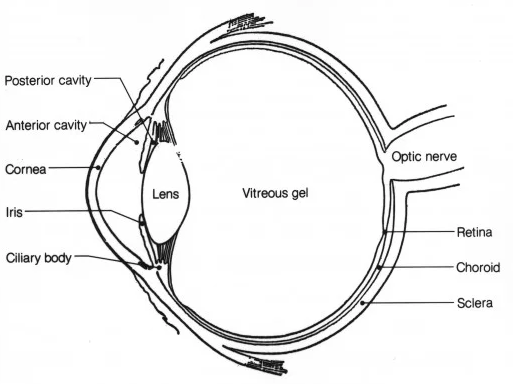
\includegraphics[width=\figwidth]{Sections/2AV1/Diagrams/eyediagram.png}
    \caption[Representation of an human eye]{Representation of an human eye \cite{owlcationAnatomyEyeHuman}.}
    \label{fig:eye}
\end{figure}

Once the desired image is properly focused by the lens, an inverse version of it is shone on the aforementioned membrane, which is covered by two types of light sensitive cells, the \emph{cones} and \emph{rods}, which transform the observable image into a series of pulses, that get subsequently processed.

The \emph{cones} are highly sensitive to color, being responsible for the \emph{photonic} or \emph{bright-light} vision. There are three different types, corresponding to the wavelength they are susceptible to. These are the \emph{S}, \emph{M} and \emph{L} \emph{cones}, being sensitive to, approximately, the blue, green and red light, respectively, making a somewhat similar capture to the RGB color system.

On the other side, \emph{rods} aren't stimulated by bright light, being more active on low illumination levels. This aspect makes them responsible for giving a rough overview of the field of view. This is called as \emph{scotopic} or \emph{dim-light} vision. These cells are more broadly spread across the retina comparing to the \emph{cones}, which is also observable in the number of cells (approximately 6 million \emph{cones}, to 100 million \emph{rods}).

From this, it's already observable that the human visual system is more sensitive to differences on the luminosity, than to the color of an object \cite{mullenContrastSensitivityHuman1985}, which is a starting point for compressing video, as will be shown later in this Chapter. However, many other opportunities come from the processing of the nerve signals, and the \emph{psychovisual} perception that follows.

Although more sensitive to \emph{luminance}, there is a threshold to which the difference between two objects --- $\Delta I$ --- can't be discerned. This relation is mentioned as \emph{contrast sensitivity function}, which is roughly approximated with the \emph{Weber's Law}

\begin{equation}
    \frac{\Delta I}{I}\approx constant
\end{equation}

Analyzing this equation, it's possible to conclude that the darker an object is, the lower the difference in luminance needs to be to distinguish another object. Also, darker images tend to be more susceptible to compression artifacts.

Besides the luminance values, the spatial and temporal frequencies also represent an important role in the perception of such errors. 

The Figure \ref{fig:noise} gives an example of the dependency with spatial frequency. The first, \ref{subfig:noiseOri}, represents the original image, which got corrupted with \gls{wgn}, represented in Figure \ref{subfig:noise}. As it is observable, these artifacts are less noticeable on the highly detailed areas (branches and leafs of the tree) than in the smooth ones (sky in the top right corner). The effect of \emph{Weber's law} is also observed if we analyze the effect that the white noise as in the bright sun area, when compared to the darker areas.

\begin{figure}[h]
    \centering
    \begin{subfigure}[c]{\textwidth}
        \centering
        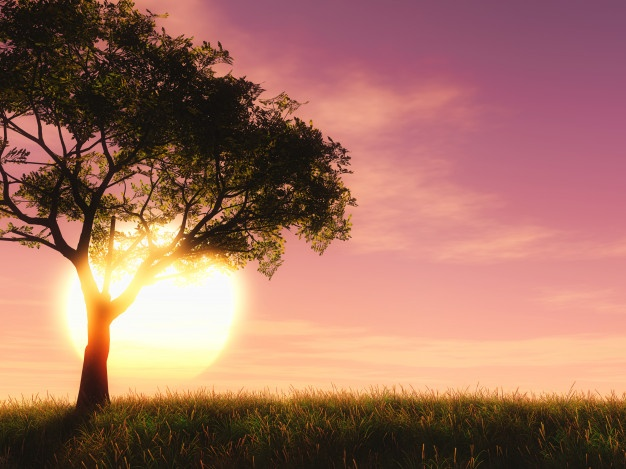
\includegraphics[width=\figwidth]{Sections/2AV1/Diagrams/paisagemOri.jpg}
        \caption{}
        \label{subfig:noiseOri}
    \end{subfigure}
    \begin{subfigure}[c]{\textwidth}
        \centering
        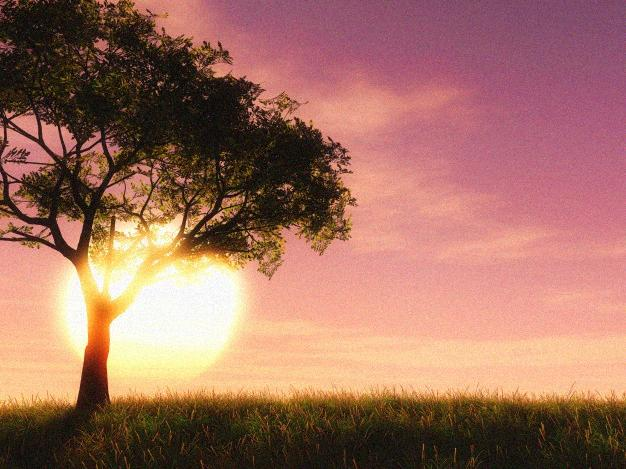
\includegraphics[width=\figwidth]{Sections/2AV1/Diagrams/paisagemNoise.jpg}
        \caption{}
        \label{subfig:noise}
    \end{subfigure}
    \caption[Example of the effect of added noise on figure]{Example of the effect of added noise on figure ((a) - Original Image \cite{Freepik}; (b) - Image with added WGN).}
    \label{fig:noise}
\end{figure}

Temporal frequency dependency, although more challenging to exemplify, is easily understandable. On a sequence of frames with fast movements, either from the camera or the subject, the human eye doesn't have the ability to track details or other artifacts, while in slow moving scenes, it can easily identify errors.

These are some of the fragilities of the human visual system that get exploited during the compression of video. However, other \emph{redundancies}, inherent from the captured images themselves contribute to the reduction of the video size, as will be described in the following sections.

%%%%%%%%%%%%%%%%%%%%%%%%%%%%%%%%%%%%%%%
\subsection{Redundancy Exploitation}

%\todo[inline,color=red!40]{*Types of redundancies (Temporal, Statistical and Coding)}
%\todo[inline,color=red!40]{*Color subsampling}
%\todo[inline,color=red!40]{*Intra-prediction}
%\todo[inline,color=red!40]{*Inter-prediction}
%\todo[inline,color=red!40]{*Transform and Quantization}
%\todo[inline,color=red!40]{*Entropy Coding}

Even though there are countless observable subjects and sceneries, it's unfair to think of a frame as a random sequence of pixels. Objects tend to represent clusters of pixels with roughly the same values, moving objects follow predictable directions, etc. Such characteristics represent \emph{redundancies} that can be explored during the compression of said sequence.

%%%%%%%%%%%%%%%%%%%
\subsubsection{Spatial Redundancy} \label{sssec:spatred}

Spatial redundancy comes from the similarity between neighboring pixels, on one frame. This aspect is easily verified through the autocorrelation of an image, as will be shown in the following example.

Taking Figure \ref{subfig:noiseOri} and calculating its autocorrelation with various horizontal shifts, gives origin to the graph in graph in Figure \ref{fig:autocorr}.

\begin{figure}[h]
    \centering
    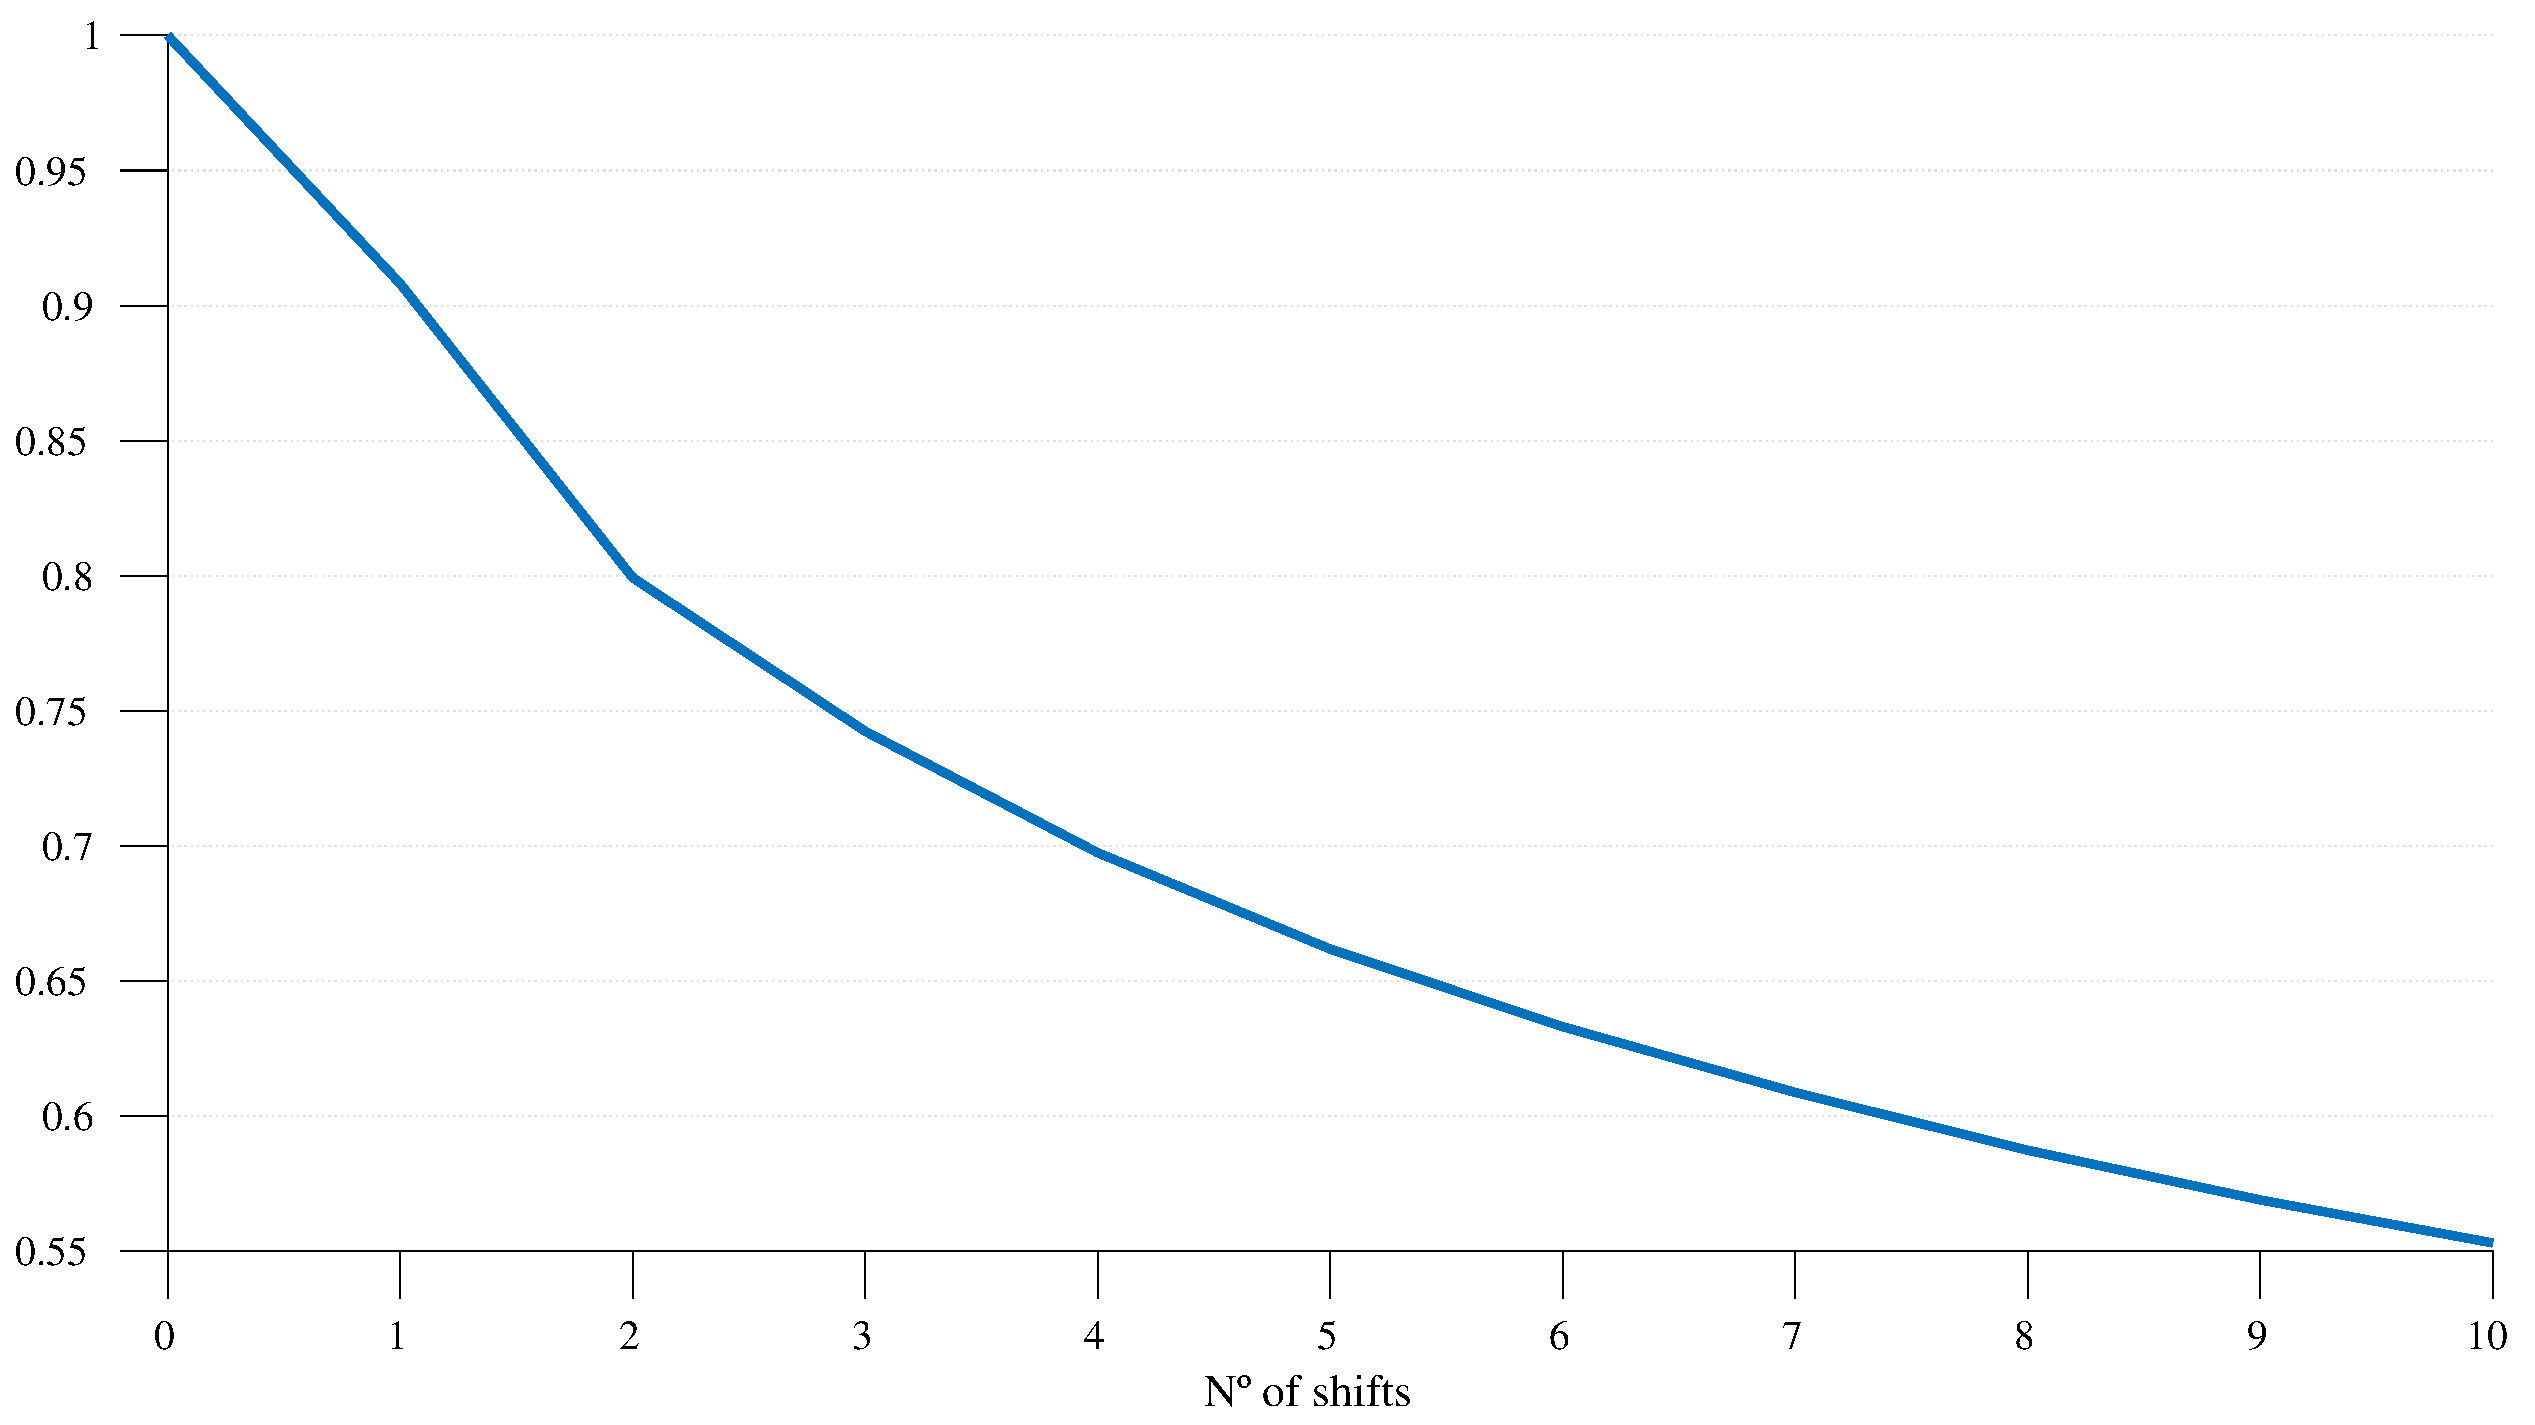
\includegraphics[width=\textwidth]{Sections/2AV1/Diagrams/intracorr.eps}
    \caption{Autocorrelation of image \ref{subfig:noiseOri}, with horizontal shifts.}
    \label{fig:autocorr}
\end{figure}

As it is observable, for shorter shifts, the normalized autocorrelation is very close to one, since most of the de-correlation comes for mismatching edges. Although this relation varies depending on the image, it's safe to assume that it is very similar for the majority of the cases.

Such study gives a promising opportunity for compression, since it means that most pixels can be predicted from its neighbors. This aspect as lead to what is now known as \emph{differential} or \emph{predictive} coding.

On a video compression system, the spatial redundancy is considered in the \emph{intra-prediction} block, which calculates pixels, or pixel blocks, through its surrounds.

%%%%%%%%%%%%%%%%%%%
\subsubsection{Temporal Redundancy}

As expected, a series of consecutive frames on the same subject, tend to be very similar between each other, especially if considered the $30$ or $60 fps$ desired nowadays. 

Making a similar analysis to what was made in Section \ref{sssec:spatred}, a series of frames of the \emph{Stefan} sequence \cite{YUVSequences} was considered, and the cross correlation between the first and the following nine was calculated, giving origin to the graph in Figure \ref{fig:crosscorr}.

\begin{figure}[h]
    \centering
    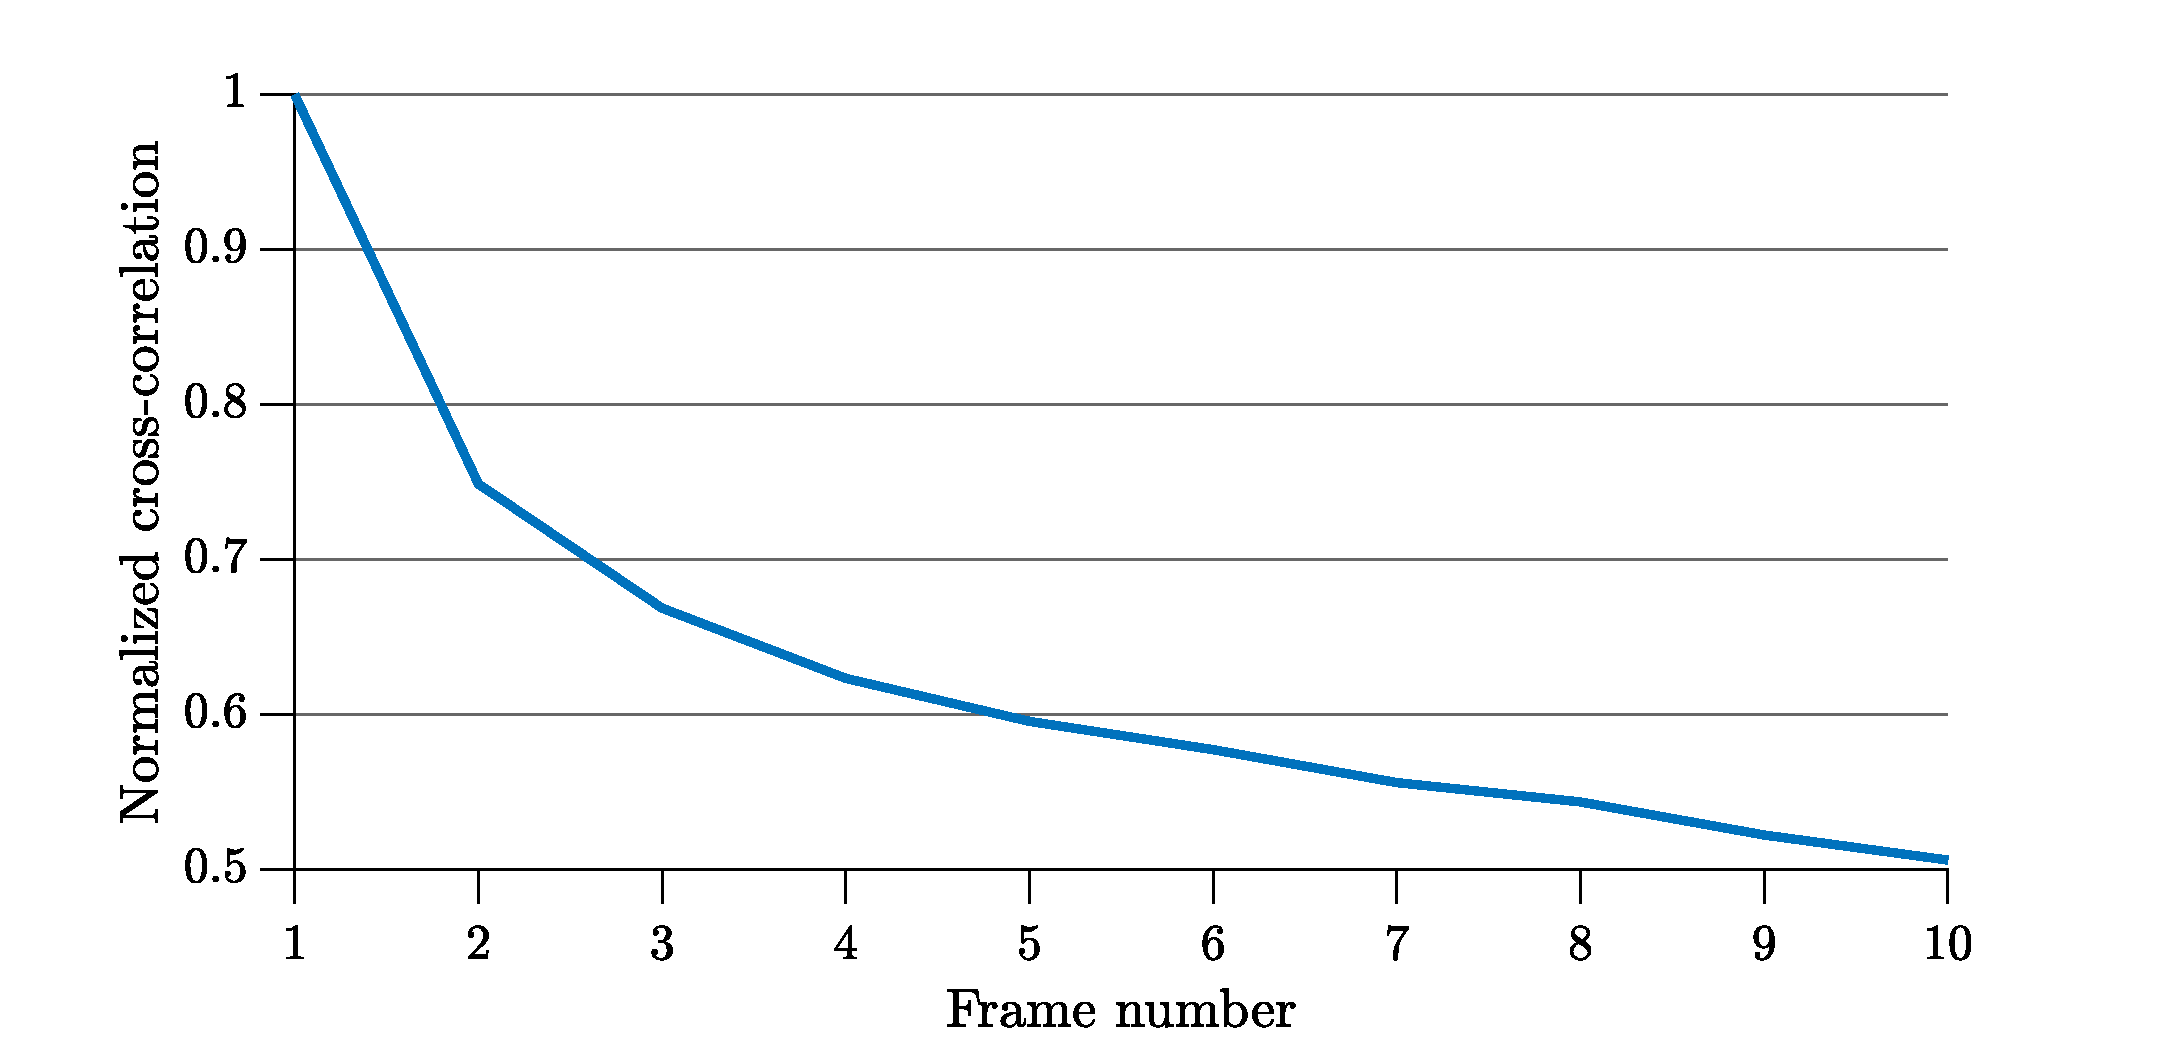
\includegraphics[width=\textwidth]{Sections/2AV1/Diagrams/intercorr.eps}
    \caption{Cross-correlation between the first and following nine frames of the \emph{Stefan} sequence.}
    \label{fig:crosscorr}
\end{figure}

Similarly to what happened in the previous example, the cross correlation between consecutive frames is very high. Even though for faster moving scenes this relation might not be as pronounced, its application on video coding greatly contributes to the compression verified in the latest codecs. 

The codec takes advantage of this redundancy in the \emph{inter-prediction} stage, which is composed by the \emph{Motion Estimation} (ME) and \emph{Motion Compensation} (MC) blocks. On this stage, blocks of pixels in nearby frames are analyzed for movement, predicting its position for following frames.

%%%%%%%%%%%%%%%%%%%
\subsubsection{Psychovisual Redundancy}

As to the redundancies presented in Section \ref{ssec:hvs}, these are explored in various stages throughout the video encoder.

The first measure is the \emph{chroma subsampling}, which takes advantage of the lower perception to color, discarding some of the \emph{chroma} samples, depending on the subsampling chosen.

Typically, a pixel value is represented in one luminance and two chrominance values, on the \emph{YCbCr} color space. The subsampling is defined in through the relation of luminance to chroma samples, being the most common the 4:4:4, 4:2:2 and 4:2:0 standards, represented in Figure \ref{fig:subsample}. In the first one, no chroma samples are discarded, which means that for each four luminance (\emph{Y}) samples, there are an equal number of \emph{Cb} and \emph{Cr} samples. Correspondingly, in the second standard, for each four Y samples, only half of each color components are maintained. The last example, although its misleading term, means that only one in four chroma samples are kept.

\begin{figure}[h]
    \centering 
        \begin{subfigure}[c]{\textwidth}
            \centering
            \begin{tikzpicture}[scale=0.75]    
    \coordinate (ycenter) at (2,3);
    \node[align=center] at (ycenter.north) {\textbf{Y}};
    \fill[gray!40] (0,0) rectangle (1,1);
    \fill[gray!70] (1,0) rectangle (2,1);
    \fill[gray!40] (2,0) rectangle (3,1);
    \fill[gray!70] (3,0) rectangle (4,1);
    \fill[gray!70] (0,1) rectangle (1,2);
    \fill[gray!40] (1,1) rectangle (2,2);
    \fill[gray!70] (2,1) rectangle (3,2);
    \fill[gray!40] (3,1) rectangle (4,2); 
    
    \coordinate (ccenter) at (7,3);
    \node[align=center] at (ccenter.north) {\textbf{Cb/Cr}};
    \fill[green!70!black] (5,0) rectangle (6,1);
    \fill[red!85!black] (6,0) rectangle (7,1);
    \fill[cyan] (7,0) rectangle (8,1);
    \fill[purple] (8,0) rectangle (9,1);
    \fill[blue!80!black] (5,1) rectangle (6,2);
    \fill[yellow!90!black] (6,1) rectangle (7,2);
    \fill[orange] (7,1) rectangle (8,2);
    \fill[brown] (8,1) rectangle (9,2);

\end{tikzpicture}
            \caption{}
            \label{subfig:444}
        \end{subfigure}
        \begin{subfigure}[c]{\textwidth}
            \centering
            \begin{tikzpicture}[scale=0.75]    
    \coordinate (ycenter) at (2,3);
    \node[align=center] at (ycenter.north) {\textbf{Y}};
    \fill[gray!40] (0,0) rectangle (1,1);
    \fill[gray!70] (1,0) rectangle (2,1);
    \fill[gray!40] (2,0) rectangle (3,1);
    \fill[gray!70] (3,0) rectangle (4,1);
    \fill[gray!70] (0,1) rectangle (1,2);
    \fill[gray!40] (1,1) rectangle (2,2);
    \fill[gray!70] (2,1) rectangle (3,2);
    \fill[gray!40] (3,1) rectangle (4,2); 
    
    \coordinate (ccenter) at (7,3);
    \node[align=center] at (ccenter.north) {\textbf{Cb/Cr}};
    \fill[green!70!black] (5,0) rectangle (6,1);
    \fill[green!70!black] (6,0) rectangle (7,1);
    \fill[cyan] (7,0) rectangle (8,1);
    \fill[cyan] (8,0) rectangle (9,1);
    \fill[blue!80!black] (5,1) rectangle (6,2);
    \fill[blue!80!black] (6,1) rectangle (7,2);
    \fill[pink] (7,1) rectangle (8,2);
    \fill[pink] (8,1) rectangle (9,2);

\end{tikzpicture}
            \caption{}
            \label{subfig:422}
        \end{subfigure}
        \begin{subfigure}[c]{\textwidth}
            \centering
            \begin{tikzpicture}[scale=0.75]    
    \coordinate (ycenter) at (2,3);
    \node[align=center] at (ycenter.north) {\textbf{Y}};
    \fill[gray!40] (0,0) rectangle (1,1);
    \fill[gray!70] (1,0) rectangle (2,1);
    \fill[gray!40] (2,0) rectangle (3,1);
    \fill[gray!70] (3,0) rectangle (4,1);
    \fill[gray!70] (0,1) rectangle (1,2);
    \fill[gray!40] (1,1) rectangle (2,2);
    \fill[gray!70] (2,1) rectangle (3,2);
    \fill[gray!40] (3,1) rectangle (4,2); 
    
    \coordinate (ccenter) at (7,3);
    \node[align=center] at (ccenter.north) {\textbf{Cb/Cr}};
    \fill[blue!80!black] (5,0) rectangle (6,1);
    \fill[blue!80!black] (6,0) rectangle (7,1);
    \fill[pink] (7,0) rectangle (8,1);
    \fill[pink] (8,0) rectangle (9,1);
    \fill[blue!80!black] (5,1) rectangle (6,2);
    \fill[blue!80!black] (6,1) rectangle (7,2);
    \fill[pink] (7,1) rectangle (8,2);
    \fill[pink] (8,1) rectangle (9,2);

\end{tikzpicture}
            \caption{}
            \label{subfig:420}
        \end{subfigure}
       \caption{Representation of chroma subsampling ((a) - 4:4:4; (b) - 4:2:2; (c) - 4:2:0).}
    \label{fig:subsample}
\end{figure}

From the reduced sensitivity to details (or areas with high spatial frequency), the compression is explored in the \emph{Transform} (T) and \emph{Quantization} (Q) blocks. In the first stage, blocks of pixels are evaluated in their frequency components. These are then evaluated in the second stage, where the least significant ones get discarded. In the decoder, the image is reconstructed with the maintained coefficients, without much impact to the image quality. This process is further explained throughout the work.

On the Quantization block, some work was also developed to account for \emph{Weber's law}, where the quantization depends on the average luminance value of the block. This concept was first introduced in \emph{"Efficiency of a Model Human Image Code"} \cite{watsonEfficiencyModelHuman1988}, and since then experimented in various codecs, such as HEVC \cite{rouisPerceptualVideoContent2018}.

%%%%%%%%%%%%%%%%%%%
\subsubsection{Coding Redundancy}

Coding redundancy is directed to the method of representing information in the digital domain, i.e., the bits themselves, and how they are organized.

It is known that symbol probability plays a major role in information compression, across a wide variety of branches, and video is no exception. Taking this into account, codecs take advantage of coding redundancy in the \emph{Entropy Encoder} stage.

%%%%%%%%%%%%%%%%%%%%%%%%%%%%%%%%%%%%%%%
\subsection{Basic Video Compression/Decompression System}

From the basic principles of the previously mentioned blocks, it is possible to integrate them into two complete compression --- \emph{Encoder} --- and decompression --- \emph{Decoder} --- modules.

%%%%%%%%%%%%%%%%%%%
\subsubsection{Encoder Model} \label{ssse:encmod}

The encoder's objective is to compress a video sequence, turning it into a readable \emph{encoded bitstream}. To do this, the previously presented strategies get implemented on a system based on the schematic of Figure \ref{fig:basicenc}.

\begin{figure}[!htbp]
    \centering
    \begin{tikzpicture}[%
    >=triangle 60,              % Nice arrows; your taste may be different
    start chain=going right,    % General flow is top-to-bottom
    node distance=2.5cm,          % Global setup of box spacing
    every join/.style={norm},   % Default linetype for connecting boxes
    scale=0.7, every node/.style={transform shape}
    ]

\tikzset{
    base/.style={draw, on chain, on grid, align=center},
    proc/.style={base, rectangle, text width=1.6cm, fill=black!15, minimum height=1.5cm, minimum width=1.5cm,font={\bfseries}},    
    frame/.style={base, minimum height=1.5cm, minimum width=2cm, fill=blue!10, thick},
    sub/.style={base, circle, inner sep=0pt, radius=0.4cm, fill=black!10, minimum height=3.5ex, font={\bfseries}},
    spot/.style={circle, inner sep=0pt, radius=0.4cm, minimum height=2mm, draw},
    edge rectangle/.style={ to path={ rectangle (\tikztotarget)}},
    % coord node style is used for placing corners of connecting lines
    coord/.style={coordinate, on chain, on grid, node distance=6mm and 40mm},
    % Arrows 
    fforw/.style={->, thick},
    fback/.style={->, thick, red!75!black},
    aref/.style={<->, dashed, black!50},
    % -------------------------------------------------
    % Connector line styles for different parts of the diagram
    cascaded/.style = {%
    general shadow = {%
      shadow scale = 1,
      shadow xshift = -1ex,
      shadow yshift = 1ex,
      draw,
      thick,
      fill = blue!40},
    general shadow = {%
      shadow scale = 1,
      shadow xshift = -.5ex,
      shadow yshift = .5ex,
      draw,
      thick,
      fill =blue!40},
    fill = blue!40, 
    draw,
    thick,
    minimum width = 2cm,
    minimum height = 1.5cm},
    base
}    

%% Top row
\node [frame] (inframe) {Input\\Frame};
    \node [coord] (ni1) {};    
    \node [coord, right=2mm of inframe.east] (ni2) {};
\node [sub, right=2cm of ni1] (sub) {-};
    \draw [fforw] (inframe) -- (sub);
\node [proc] (T) {T};
    \draw [fforw] (sub) -- (T);
\node [proc] (Q) {Q};
    \draw [fforw] (T) -- (Q);
\coordinate (rq) at ($(Q.east)+(4mm,0)$);
\node [proc, right=1cm of Q.east] (EC) {Entropy\\Coding};
    \draw [fforw] (Q) -- (EC);
\coordinate (out) at ($(EC.east)+(4mm,0)$);
%\path (EC) to node [yshift=-1em] {Encoded\\Bitstream} (out);
    \draw [fforw] (EC) -- (out);

%% Reference
\node [cascaded, below=5cm of inframe] (ref) {Reference\\Frames};

%% Intra
\node [proc, below=1.5cm of ni1] (intra) {Intra\\Coding};
    \coordinate (ni3) at (ni2 |- intra);    
    \draw [fforw] (ni3) -- (intra);

%% Inter    
\node [proc,right=of ref] (inter) {Inter\\Coding};
    \node [coord, below=4.5cm of ni2] (ni4) {};
    \draw [fforw] (ni2) -- (ni4) |- ($(inter.west)+(0,5mm)$);
    \draw [fforw] ($(ref.east)+(0,-5mm)$) -- ($(inter.west)+(0,-5mm)$);

%% Selector
\coordinate (rintra) at ($(intra.east)+(5mm,0)$);
\node [spot, below=1cm of rintra, fill=black] (sintra) {};
    \draw [thick] (intra.east) -- (rintra) |- (sintra.north);

\coordinate (rinter) at ($(inter.east)+(5mm,0)$);
\node [spot, above=1cm of rinter, fill=black] (sinter) {};
    \draw [thick] (inter.east) -- (rinter) |- (sinter.south);

\path (sintra) -- (sinter) coordinate [midway] (intraintermid);
\node [spot, at=(sub |- intraintermid)] (sel) {};
\draw [dashed] ($(sel)+(-4mm,3.3mm)$) arc (140:220:5mm);
    \draw [fforw] (sintra) -- (sel);
    \draw [fforw] (sel) -- (sub);

%% Lower Row    
\node [sub, below=3.7cm of sel] (add) {+};
    \draw [fback] (sel) -- (add);
\node [proc] (T1) {$\mathbf{T^{-1}}$};
    \draw [fback] (T1) -- (add);
\node [proc] (Q1) {$\mathbf{Q^{-1}}$};
    \draw [fback] (Q1) -- (T1);
\coordinate (rq1) at ($(Q1.east)+(4mm,0)$);
    \draw [fback] (rq) -- (rq1) |- (Q1);
\node [frame, below=7.4cm of inframe] (recframe) {Reconstructed\\Frame};
    \draw [fback] (add) -- (recframe);
\end{tikzpicture}
    \caption{Simplified Basic Encoder Model.}
    \label{fig:basicenc}
\end{figure}

The encoding process starts with the \emph{Input Frame}, which can be of two types. \emph{I Frames} are encoded using only the information present in themselves, i.e., using only \emph{Intra Prediction/Coding}, while \emph{P Frames} may use predictive coding from previously encoded frames \footnote{Most video codecs allow the encoding sequence to be different from the temporal sequence. This allows the currently encoding frame to use reference frames displayed after itself.}.

The input gets split into blocks, which get fed into the two main blocks of a video encoder: the \emph{Intra} and \emph{Inter} Prediction blocks.

The \emph{Intra Coding} block, as mentioned previously, deals with the spatial redundancy, by predicting the current block from the pixels above and to the left of its upper and left edges. The prediction may be done with various algorithms, ranging from calculating the average from the reference pixels, to replicating these according to a certain direction. One such example is presented in Figure \ref{fig:intraex}, where pixels B through H get spread across a $4\times 4$ block, diagonally.

\begin{figure}[!htbp]
    \centering
    \begin{tikzpicture}[scale=0.7,>=triangle 60]
\tikzset{
    a/.style={->},
}    
    \draw [fill=lightgray] (0,0) rectangle (1,5);
    \draw [fill=lightgray] (1,4) rectangle (9,5);
    \draw[step=1cm,black,very thin] (0,0) grid (5,5);
    \draw[step=1cm,black,very thin] (5,4) grid (9,5);

    \node at (1.5,4.5) {A};
    \node at (2.5,4.5) {B};
    \node at (3.5,4.5) {C};
    \node at (4.5,4.5) {D};
    \node at (5.5,4.5) {E};
    \node at (6.5,4.5) {F};
    \node at (7.5,4.5) {G};
    \node at (8.5,4.5) {H};

    \node at (0.5,4.5) {I};
    \node at (0.5,3.5) {J};
    \node at (0.5,2.5) {K};
    \node at (0.5,1.5) {L};
    \node at (0.5,0.5) {M};

    \draw [a] (8,4) --(4,0);
    \draw [a] (7,4) --(3,0);
    \draw [a] (6,4) --(2,0);
    \draw [a] (5,4) --(1,0);
    \draw [a] (4,4) --(1,1);
    \draw [a] (3,4) --(1,2);
    \draw [a] (2,4) --(1,3);
\end{tikzpicture}
    \caption{Directional Intra-prediction example.}
    \label{fig:intraex}
\end{figure}

Into the \emph{Inter Coding} block, go two inputs. The currently encoding block, as well as a bank of previously encoded frames, named \emph{Reference Frames}. Firstly, the frames inside the buffer get searched for blocks resembling the former input. Once found, this process generates a \emph{motion vector}, corresponding to the difference between the position of the block found in the reference frame, and the position of the currently encoding block, as shown in Figure \ref{fig:interex}.

\begin{figure}[!htbp]
    \centering
    \begin{tikzpicture}[scale=.7,every node/.style={minimum size=1cm},on grid,>=triangle 60]
		
    %slanting: production of a set of n 'laminae' to be piled up. N=number of grids.
    \begin{scope}[
            yshift=-83,every node/.append style={
            yslant=0.5,xslant=-1},yslant=0.5,xslant=-1
            ]
        % opacity to prevent graphical interference
        \fill[white,fill opacity=0.9] (0,0) rectangle (5,5);
        \draw[blue!40!black,very thick] (0,0) rectangle (5,5);%marking borders
        \filldraw[blue!30] (0.5,0.5) rectangle (1.5,1.5);
        \draw[gray, dashed] (0.5,1.5) -- (3.42,4.42);
        \draw[gray, dashed] (1.5,0.5) -- (4.42,3.42);
        \draw[gray, dashed] (0.5,0.5) -- (3.42,3.42);
        \draw[gray, dashed] (1.5,1.5) -- (4.42,4.42);
        %Idem as above, for the n-th grid:
    \end{scope}
    
    \begin{scope}[
    	    yshift=0,every node/.append style={
    	    yslant=0.5,xslant=-1},yslant=0.5,xslant=-1
            ]
        \fill[white,fill opacity=.9] (0,0) rectangle (5,5);
        \draw[black,very thick] (0,0) rectangle (5,5);

        \draw[blue!30] (0.5,0.5) rectangle (1.5,1.5);
        \filldraw[gray] (2.5,3) rectangle (3.5,4);

        \draw[->] (0.5,0.5) -- (2.5,3);
    \end{scope}

    \draw[-latex,thick](5.8,0)node[right]{Reference Frame}
    to[out=180,in=90] (3.4,-1);

    \draw[-latex,thick] (5.8,3) node[right]{Present Frame}
         to[out=180,in=90] (3.4,2);

    \draw[-latex,thick] (-5.5,2.2) node[left]{Motion Vector}
    to [out=0,in=180](-0.22,1.5);
\end{tikzpicture}
    \caption{Inter-prediction example.}
    \label{fig:interex}
\end{figure}

In most codecs, the motion vector has a precision below one pixel. This means that the matching block, from the reference frame, may be interpolated from existing pixels. This process is known as \emph{sub-pixel interpolation}, which calculates virtual values between existing pixels. 

After the prediction stage, the chosen output between the two processes, i.e., the predicted block, gets subtracted by the current one, giving origin to the \emph{residue}. This corresponds to the pixel value differences between the original and predicted blocks. Lower \emph{residues} indicate more efficient prediction stages.

The next stage, the \emph{Forward Transform}, is the focus of this work. It takes the residue blocks, which may not be the same size of the prediction blocks, and evaluates them according to its spatial frequencies. Its output corresponds to a series of \emph{coefficients}, that are related to the similarity --- or \emph{correlation} --- between the input block and a series of \emph{basis images}. This process is further explained in Chapter \ref{chap:trans}.

On the \emph{Quantization} stage, the coefficients calculated in \textbf{T} get scaled according to a \emph{Quantization Matrix}. This stage takes advantage of the eye's lower perception to details, and scales the higher frequency coefficients by a higher value, than the lower, more significant ones. In most of the transformed blocks, this leads to only a few low frequency components being maintained, while the others get nullified, since they are not relevant to the reconstruction of the image. Therefore, this stage is the the one that presents the higher loss, although the previously presented also introduce errors. In most of the encoding processes, this stage has the most direct impact on the obtained quality.

The wipe out of the least significant coefficients is particularly efficient when paired with the last stage before the output, the \emph{Entropy Encoder}. On this block, \textbf{Q}'s output blocks get run sequentially via a \emph{zig-zag scan}, which first passes through the lower frequency coefficients, followed by the higher frequency ones, as demonstrated by Figure \ref{fig:zigzag}.

\begin{figure}[!htbp]
    \centering
    \begin{tikzpicture}[scale=0.7,>=triangle 60]
    \tikzset{
        a/.style={>->, thick},
    }    
        \draw[step=1cm,black,very thin] (0,0) grid (8,8);
    
        \draw [a] (0.5,7.5) -- (1.5,7.5) -- (0.5,6.5) -- (0.5,5.5) -- (2.5,7.5) -- (3.5,7.5) -- (0.5,4.5) -- (0.5,3.5) -- (4.5,7.5) -- (5.5,7.5) -- (0.5,2.5) -- (0.5,1.5) -- (6.5,7.5) -- (7.5,7.5) -- (0.5,0.5) -- (1.5,0.5) -- (7.5,6.5) -- (7.5,5.5) -- (2.5,0.5) -- (3.5,0.5) -- (7.5,4.5)  -- (7.5,3.5) -- (4.5,0.5)  -- (5.5,0.5) -- (7.5,2.5) -- (7.5,1.5)  -- (6.5,0.5)  -- (7.5,0.5);

        \draw [->, -latex] (3,8.5) -- node[above, font={\small}]{Horizontal Frequency ($u$)} (5,8.5);

        \draw [->, -latex] (-0.5,5) -- node[above, font={\small}, rotate=90]{Vertical Frequency ($v$)} (-0.5,3);
    \end{tikzpicture}
    \caption{Demonstration of Zig-Zag Scan.}
    \label{fig:zigzag}
\end{figure}

In most of the cases, this causes that the non-zero coefficients get read first, followed by a sequence of zeros. Such sequence benefits heavily of being encoded with \gls{vlc}, such as \emph{Huffman Tree Codes} or \Gls{cabac}. Off all the processes, this is the one that doesn't introduce further distortion into the encoded sequence, which is the reason it doesn't get included in the \emph{feedback loop}.

The intent of this loop is to get an exact same copy of the frame reconstructed in the decoder. This reconstructed frame gets used as the reference for intra-prediction, or gets put into the reference frame buffer to be used in a later inter-prediction process. 

The output of the encoder is the quantized coefficients, as well as the necessary information to recreate the encoded blocks, such as the type of prediction used, the transformation \emph{kernel} [see p.\pageref{par:kernel}], quantization matrix, et al. These encoding parameters are the choices made by the \emph{Control Unit}, which although represented by a block in Figure \ref{fig:basicenc}, may not be a local process, independent from all others. 

Since \emph{H.264}, most video codecs standardize the decoding process, specifically the allowed tools for reconstructing the video, and how to use them. This means that the encoding process is widely adaptable to the compression objectives, as long as the final product is a bitstream following the norms set on the codec's standard \cite{AV1BitstreamDecoding}. Therefore, the definition of a \emph{Control Unit} is ambiguous in this context, since such unit can simply represent a set of parameters to be used throughout the encoding process\footnote{One such example would be \emph{lossless} compression modes, which use very a concise conditions on each stage, in order to get the least distortion.}, or an algorithm that can change between the different capabilities of the codec, in order to achieve an objective, such as a specific distortion rate, or not surpass a maximum bit rate. As expected, different objectives may lead to majorly different results, both in the output video, as well as in the used tools.

%%%%%%%%%%%%%%%%%%%
\subsubsection{Decoder Model}

As expected, the decoder (Figure \ref{fig:basicdec}) does the backwards operation of the encoder on Figure \ref{fig:basicenc}. It starts by analyzing the bitstream, separating the control information from the encoded and quantized coefficients.

\begin{figure}[!htbp]
    \centering
    \begin{tikzpicture}[%
    >=triangle 60,              % Nice arrows; your taste may be different
    start chain=going right,    % General flow is top-to-bottom
    node distance=2.5cm,          % Global setup of box spacing
    every join/.style={norm},   % Default linetype for connecting boxes
    ]

\tikzset{
    base/.style={draw, on chain, on grid, align=center},
    proc/.style={base, rectangle, text width=1.6cm, fill=black!15, minimum height=1.5cm, minimum width=1.5cm,font={\bfseries}},    
    frame/.style={base, minimum height=1.5cm, minimum width=2cm, fill=blue!10, thick},
    sub/.style={base, circle, inner sep=0pt, radius=0.4cm, fill=black!10, minimum height=3.5ex, font={\bfseries}},
    spot/.style={circle, inner sep=0pt, radius=0.4cm, minimum height=2mm, draw},
    edge rectangle/.style={ to path={ rectangle (\tikztotarget)}},
    % coord node style is used for placing corners of connecting lines
    coord/.style={coordinate, on chain, on grid, node distance=6mm and 40mm},
    % Arrows 
    fforw/.style={->, thick},
    fback/.style={->, thick, red!75!black},
    aref/.style={<->, dashed, black!50},
    % -------------------------------------------------
    % Connector line styles for different parts of the diagram
    cascaded/.style = {%
    general shadow = {%
      shadow scale = 1,
      shadow xshift = -1ex,
      shadow yshift = 1ex,
      draw,
      thick,
      fill = blue!40},
    general shadow = {%
      shadow scale = 1,
      shadow xshift = -.5ex,
      shadow yshift = .5ex,
      draw,
      thick,
      fill =blue!40},
    fill = blue!40, 
    draw,
    thick,
    minimum width = 2cm,
    minimum height = 1.5cm},
    base
}    

\node [coord] (ed) {};    
\node[proc, text width=2cm, right=4mm of ed] (ED) {Entropy\\Decoding};
    \draw [fforw] (ed) -- (ED.west);
\node [proc] (Q1) {$\mathbf{Q^{-1}}$};
    \draw [fforw] (ED) -- (Q1);
\node [proc] (T1) {$\mathbf{T^{-1}}$};
    \draw [fforw] (Q1) -- (T1);
\node [sub] (add) {+};
    \draw [fforw] (T1) -- (add);
\node [frame, right=5cm of add] (recframe) {Reconstructed\\Frame};
    \draw [fforw] (add) -- (recframe);

%% Inter
\node [cascaded, below=5cm of recframe] (ref) {Reference\\Frames};
\node [proc, left=of ref] (inter) {Inter\\Coding};
\draw [fforw] (ref) -- (inter);

%% Intra
\coordinate (lrec) at (inter |- recframe);
\node [proc, below=1.5cm of lrec] (intra) {Intra\\Coding};
    \draw [fforw] (intra |- recframe) -- (intra.north);

%% Selector
\coordinate (lintra) at ($(intra.west)+(-5mm,0)$);
\node [spot, below=1cm of lintra, fill=black] (sintra) {};
    \draw [thick] (intra.west) -- (lintra) |- (sintra.north);

\coordinate (linter) at ($(inter.west)+(-5mm,0)$);
\node [spot, above=1cm of linter, fill=black] (sinter) {};
    \draw [thick] (inter.west) -- (linter) |- (sinter.south);

\path (sintra) -- (sinter) coordinate [midway] (intraintermid);
\node [spot, at=(add |- intraintermid)] (sel) {};
\draw [dashed] ($(sel)+(4mm,-3.3mm)$) arc (-40:40:5mm);
    \draw [fforw] (sintra) -- (sel);
    \draw [fforw] (sel) -- (add);

%% Control
\path (ED.west) -- (recframe.east) node[midway] (mid) {};
\node [proc, text width=8cm, fill=black!40, above=2cm of mid, rounded corners, ] (control) {Control Unit};
    \draw [aref] (T1) -- (T1.north |- control.south);
    \draw [aref] (Q1) -- (Q1.north |- control.south);
\coordinate (aboved) at (ED |- control);
    \draw [aref] (ED) -- (aboved) |- (control);
    \draw [aref] (intra.120) -- (intra.120 |- control.south);
    \draw [aref] (inter.south) -- ++(0,-3.2mm) coordinate (y) |- (control.south |- y) |- (control.south);
    \draw [aref] (sel.west) -- ++(-6mm,0) coordinate (y) |- (y |- control.south);

%% Legend
\node [below=5cm of ED, font={\tiny}] (lc) {Control\\Signal};
    \draw [aref] ($(lc.west)+(-6mm,0)$) -- +(5mm,0);
\node [above=7mm of lc, font={\tiny}] (lf) {Forward\\Path};
    \draw [fforw] ($(lc.west)+(-6mm,7mm)$) -- +(5mm,0); 
\draw[thick] ($(lc.south west)+(-9mm,-2mm)$) rectangle ($(lf.north east)+(2mm,2mm)$);

\end{tikzpicture}
    \caption{Simplified Basic Decoder Model.}
    \label{fig:basicdec}
\end{figure}

Having the encoding choices performed by the encoder, the decoder returns the \emph{coding redundancy} to the quantized coefficients, on the \emph{Entropy Decoding} stage. This corresponds to a translation from the varying length code used in codification, back into the raw coefficients.

The \emph{Inverse Quantization} rescales the maintained coefficients, resulting from the previous \emph{Quantization} stage. With this, it is meant that the same quantization matrix used when dividing the transformed coefficients, in the encoder, is now multiplied by the quantized parameters. It must be kept in mind that this operation does not output an exact copy of the transformation coefficients, as a lot of information is permanently lost in \textbf{Q}. This process can be seen in Figure \ref{fig:quant}.

\begin{figure}[!htbp]
    \centering
    \begin{tikzpicture}[scale=0.5,>=triangle 60]
    \def\intrans{
        {19, -1, 0, 1, -1, 8, 3, -3, -3, -2, 1, -7, -3, -4, 8, 0}
    }
    \tikzset{
        a/.style={>->, thick},
    }    
    \node (inres) [inner sep=0pt, draw, label={[align=center, font={\small\bfseries}]above:Input\\Residue}, fit={(0,0) (4,4)}] {};
        \draw[step=1cm,black,very thin, inner sep=0pt] (0,0) grid (4,4);   
            \node at (0.5, 0.5) {6};
            \node at (0.5, 1.5) {-3};
            \node at (0.5, 2.5) {5};
            \node at (0.5, 3.5) {6};
            \node at (1.5, 0.5) {0};
            \node at (1.5, 1.5) {9};
            \node at (1.5, 2.5) {8};
            \node at (1.5, 3.5) {8};
            \node at (2.5, 0.5) {8};
            \node at (2.5, 1.5) {7};
            \node at (2.5, 2.5) {-2};
            \node at (2.5, 3.5) {5};
            \node at (3.5, 0.5) {7};
            \node at (3.5, 1.5) {7};
            \node at (3.5, 2.5) {6};
            \node at (3.5, 3.5) {-1};
    
    \node [inner sep=0pt, draw, right=1 of inres, label={[align=center, font={\small\bfseries}]above:Transformed\\Coefficients}, fit={(5,0) (9,4)}] (intrans) {};
        \draw[step=1cm,black,very thin, inner sep=0pt] (intrans.south west) grid (intrans.north east);   
                    \node at ($(intrans.south west)+(0.5,0.5)$) {1};
                    \node at ($(intrans.south west)+(0.5,1.5)$) {0};
                    \node at ($(intrans.south west)+(0.5,2.5)$) {-1};
                    \node at ($(intrans.south west)+(0.5,3.5)$) {19};
                    \node at ($(intrans.south west)+(1.5,0.5)$) {-3};
                    \node at ($(intrans.south west)+(1.5,1.5)$) {3};
                    \node at ($(intrans.south west)+(1.5,2.5)$) {8};
                    \node at ($(intrans.south west)+(1.5,3.5)$) {-1};
                    \node at ($(intrans.south west)+(2.5,0.5)$) {-7};
                    \node at ($(intrans.south west)+(2.5,1.5)$) {1};
                    \node at ($(intrans.south west)+(2.5,2.5)$) {-2};
                    \node at ($(intrans.south west)+(2.5,3.5)$) {-3};
                    \node at ($(intrans.south west)+(3.5,0.5)$) {0};
                    \node at ($(intrans.south west)+(3.5,1.5)$) {8};
                    \node at ($(intrans.south west)+(3.5,2.5)$) {-4};
                    \node at ($(intrans.south west)+(3.5,3.5)$) {-3};

    \node [draw, circle, fill=lightgray, right=1 of intrans, minimum height=0.5, font={\bfseries}] (div) {$\div$};

    \node [inner sep=0pt, draw, below right=3 and 3 of div, label={[align=center, font={\small\bfseries}]above:Quantized\\Coefficients}, fit={(11,0) (15,4)}] (inq) {};
        \draw[step=1cm,black,very thin, inner sep=0pt] (inq.south west) grid (inq.north east);   
                \node at ($(inq.south west)+(0.5,0.5)$) {0};
                \node at ($(inq.south west)+(0.5,1.5)$) {0};
                \node at ($(inq.south west)+(0.5,2.5)$) {-1};
                \node at ($(inq.south west)+(0.5,3.5)$) {19};
                \node at ($(inq.south west)+(1.5,0.5)$) {-1};
                \node at ($(inq.south west)+(1.5,1.5)$) {1};
                \node at ($(inq.south west)+(1.5,2.5)$) {3};
                \node at ($(inq.south west)+(1.5,3.5)$) {-1};
                \node at ($(inq.south west)+(2.5,0.5)$) {-1};
                \node at ($(inq.south west)+(2.5,1.5)$) {0};
                \node at ($(inq.south west)+(2.5,2.5)$) {0};
                \node at ($(inq.south west)+(2.5,3.5)$) {-1};
                \node at ($(inq.south west)+(3.5,0.5)$) {0};
                \node at ($(inq.south west)+(3.5,1.5)$) {1};
                \node at ($(inq.south west)+(3.5,2.5)$) {-1};
                \node at ($(inq.south west)+(3.5,3.5)$) {-1};

    \node [inner sep=0pt, draw, below left=3 and 2 of div, label={[align=center, font={\small\bfseries}]above:Quantization\\Matrix}, fit={(11,0) (15,4)}] (qm) {};
        \draw[step=1cm,black,very thin, inner sep=0pt] (qm.south west) grid (qm.north east);   
            \node at ($(qm.south west)+(0.5,0.5)$) {4};
            \node at ($(qm.south west)+(0.5,1.5)$) {3};
            \node at ($(qm.south west)+(0.5,2.5)$) {2};
            \node at ($(qm.south west)+(0.5,3.5)$) {1};
            \node at ($(qm.south west)+(1.5,0.5)$) {5};
            \node at ($(qm.south west)+(1.5,1.5)$) {4};
            \node at ($(qm.south west)+(1.5,2.5)$) {3};
            \node at ($(qm.south west)+(1.5,3.5)$) {2};
            \node at ($(qm.south west)+(2.5,0.5)$) {7};
            \node at ($(qm.south west)+(2.5,1.5)$) {6};
            \node at ($(qm.south west)+(2.5,2.5)$) {6};
            \node at ($(qm.south west)+(2.5,3.5)$) {3};
            \node at ($(qm.south west)+(3.5,0.5)$) {9};
            \node at ($(qm.south west)+(3.5,1.5)$) {8};
            \node at ($(qm.south west)+(3.5,2.5)$) {7};
            \node at ($(qm.south west)+(3.5,3.5)$) {6};
    
    \node [inner sep=0pt, draw, below left=6 and 2 of div, label={[align=center, font={\small\bfseries}]above:Restored\\Coefficients}, fit={(11,0) (15,4)}] (outq) {};
        \draw[step=1cm,black,very thin, inner sep=0pt] (outq.south west) grid (outq.north east);   
            \node at ($(outq.south west)+(0.5,0.5)$) {0};
            \node at ($(outq.south west)+(0.5,1.5)$) {0};
            \node at ($(outq.south west)+(0.5,2.5)$) {-2};
            \node at ($(outq.south west)+(0.5,3.5)$) {19};
            \node at ($(outq.south west)+(1.5,0.5)$) {-5};
            \node at ($(outq.south west)+(1.5,1.5)$) {4};
            \node at ($(outq.south west)+(1.5,2.5)$) {9};
            \node at ($(outq.south west)+(1.5,3.5)$) {-2};
            \node at ($(outq.south west)+(2.5,0.5)$) {-7};
            \node at ($(outq.south west)+(2.5,1.5)$) {0};
            \node at ($(outq.south west)+(2.5,2.5)$) {0};
            \node at ($(outq.south west)+(2.5,3.5)$) {-3};
            \node at ($(outq.south west)+(3.5,0.5)$) {0};
            \node at ($(outq.south west)+(3.5,1.5)$) {8};
            \node at ($(outq.south west)+(3.5,2.5)$) {-7};
            \node at ($(outq.south west)+(3.5,3.5)$) {-6};

    \node [draw, circle, fill=lightgray, right=of outq, minimum height=0.5, font={\bfseries}] (mul) {$\times$};

    \node [inner sep=0pt, draw, left=of outq, label={[align=center, font={\small\bfseries}]above:Restored\\Residue}, fit={(2,-12) (6,-8)}] (outt) {};
    \draw[step=1cm,black,very thin, inner sep=0pt] (outt.south west) grid (outt.north east);   
        \node at ($(outt.south west)+(0.5,0.5)$) {5};
        \node at ($(outt.south west)+(0.5,1.5)$) {-5};
        \node at ($(outt.south west)+(0.5,2.5)$) {5};
        \node at ($(outt.south west)+(0.5,3.5)$) {5};
        \node at ($(outt.south west)+(1.5,0.5)$) {1};
        \node at ($(outt.south west)+(1.5,1.5)$) {9};
        \node at ($(outt.south west)+(1.5,2.5)$) {9};
        \node at ($(outt.south west)+(1.5,3.5)$) {10};
        \node at ($(outt.south west)+(2.5,0.5)$) {10};
        \node at ($(outt.south west)+(2.5,1.5)$) {7};
        \node at ($(outt.south west)+(2.5,2.5)$) {-4};
        \node at ($(outt.south west)+(2.5,3.5)$) {2};
        \node at ($(outt.south west)+(3.5,0.5)$) {6};
        \node at ($(outt.south west)+(3.5,1.5)$) {9};
        \node at ($(outt.south west)+(3.5,2.5)$) {7};
        \node at ($(outt.south west)+(3.5,3.5)$) {0};


    \draw [->, very thick, gray] (inres.east)+(0.5,0) -- node[above]{\textbf{T}} +(2.5,0);
    \draw [->] (intrans.east)+(0.5,0) -- +(1.5,0);
    \draw [->] ($(qm.east)+(0.5,0)$) -- (div |- qm) |- ($(div.south)+(0,-0.5)$);
    \draw [->] ($(qm.east)+(0.5,0)$) -- (div |- qm) -| ($(mul.north)+(0,0.5)$);
    \draw [->, very thick, gray] ($(div)+(-45:1)$) -- node[above,sloped,near start]{\textbf{Q}} ($(inq.west)+(-0.2,0.4)$);
    \draw [->] ($(inq.west)+(-0.2,-0.4)$) -- ($(mul)+(45:1)$);
    \draw [->, very thick, gray] (mul.west)+(-0.5,0) -- node[above,sloped,yshift=3]{$\mathbf{Q^{-1}}$} +(-1.5,0);
    \draw [->, very thick, gray] (outq.west)+(-0.5,0) -- node[above,sloped,yshift=3]{$\mathbf{T^{-1}}$} +(-2.5,0);
\end{tikzpicture}
    \caption{Processing of $\protect 4\times 4$ residue block from \emph{transformation} to restoring.} 
    \label{fig:quant}
\end{figure}

As can also be seen in this Figure, the \emph{Inverse Transform} converts the coefficients back into spatial coordinates, therefore getting the restored residue. To obtain the final approximation of the block being decoded, this residue must be added to the same predicted block from the encoder. To do so, the \emph{Intra} or \emph{Inter Prediction} stages act according to the choices made in the encoding process, as to regenerate this block.

In the decoder, the \emph{Control Unit} represents the process that organizes the different stages, according to the choices done in the encoding stage.

\nocite{agostiniDesenvolvimentoArquiteturasAlto2007}

%%%%%%%%%%%%%%%%%%%%%%%%%%%%%%%%%%%%%%%%%%%%%%%%%%%%%%%%%%%%%%%%%%%%%%%%%%%%%%
\section{AV1}

Being the focus of this work, in the following sections, \emph{AV1} is presented on its most relevant aspects, starting with its development process.

%%%%%%%%%%%%%%%%%%%%%%%%%%%%%%%%%%%%%%%
\subsection{History and Development}

\nocite{debarghamukherjeeAllThingsRTC2019Opening2019}

The development of this codec started as a need to improve the bandwidth reduction of \emph{VP9}. Therefore, the presentation of \emph{AV1} starts by explaining the guidelines of its predecessor.

\emph{VP9} started with project \emph{Webm}, created by \emph{On2}, which got acquired by \emph{Google} in 2010. This project had the objective of developing the first\footnote{VP8 got openly released after the acquisition of the company, after closing the development process.} open-source, royalty-free video codec. This got support from major video content producers, such as \emph{YouTube}, \emph{Netflix} and \emph{Twitch}, since it represented large savings in licensing payments, from the use of MPEG's standards, which got aggravated from the difficult patenting terms of \emph{HEVC} \cite{streamingmediaHEVCAdvancePatent2015}. After release in 2013, \emph{VP9} got adopted as \emph{YouTube}'s default video codec for video's above \emph{420p}, as well as other web-video consumption services, including \emph{Facebook}.

In 2014, \emph{Google} started working on the next generation of open-source video codecs, \emph{VP10}. However, due to the large interest from other companies which already used the previous standard, in 2015, the \emph{Alliance for Open Media} was created, and the the development made for this standard got inserted into \emph{AV1}. Alongside \emph{Google}, twelve other companies started \emph{AOM}, including two which also had open video encoder projects, which also majorly contributed to the fast development of \emph{AV1}: \emph{Cisco}'s \emph{Thor} and \emph{Mozilla}'s \emph{Daala}. As the time of writing, 42 companies are official members of \emph{AOM}, englobing a wide range of markets, from video streaming services, to hardware producers.

\begin{figure}[!htbp]
    \centering
    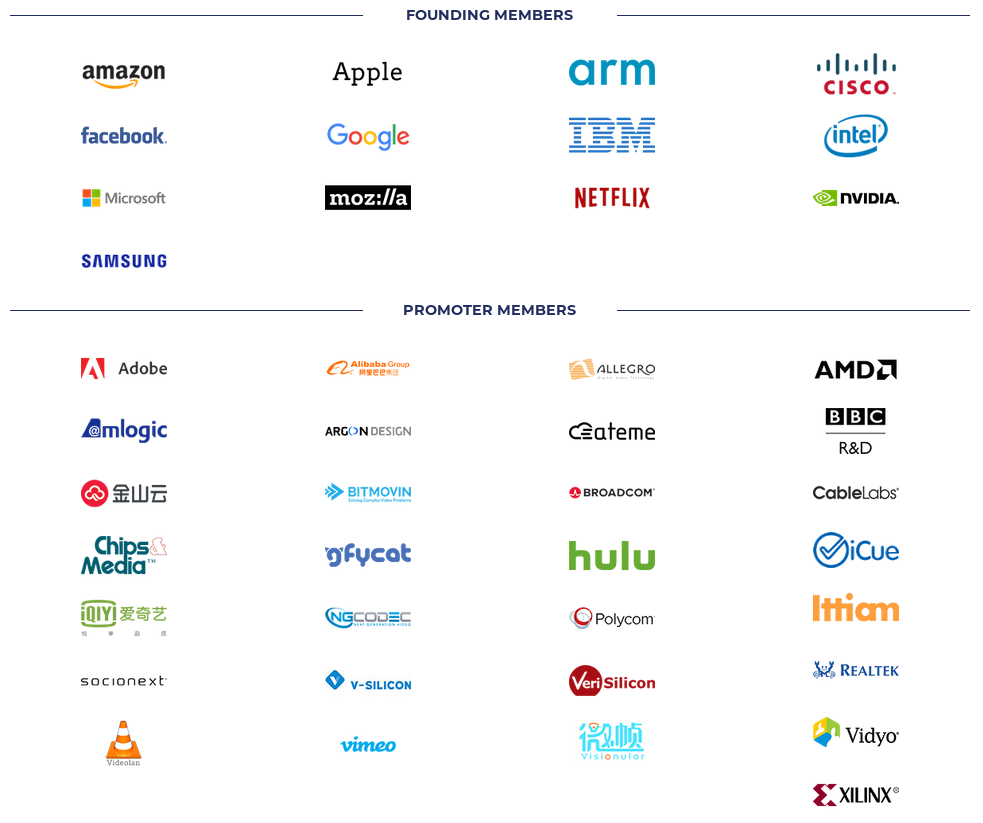
\includegraphics[width=\textwidth]{Sections/2AV1/Diagrams/Images/AOM.png}
    \caption[\emph{Alliance for Open Media} current members]{\emph{Alliance for Open Media} current members \cite{aomediaHome}.} 
    \label{fig:aom}
\end{figure}

By 2016, \emph{AV1} started, with the objective of reaching 30\% bitrate decrease, in comparison to \emph{VP9}. After the bitstream freeze in March 2018 and deployment of \emph{libaom} soon later, this first objective was fulfilled. However, the compression performance did not atone for the very high compression and decompression times of the reference software. This left a large margin for improvement, which quickly got explored with the development of other compression and decompression algorithms by the \emph{AOM} members, such as \emph{dav1d}, \emph{rav1e}, \emph{SVT-AV1},  among others. This parallel development gave origin to a competition among the corresponding teams, that benefited the adoption of the standard, since it brought a wide range of possibilities. 

With the improvements verified on both encoders and decoders, \emph{AV1} got progressively more adoption from the industry, getting support from most web browsers, as well as uploads of \emph{AV1} encoded videos to streaming platforms \cite{eggeLatestTechnicalBusiness2019}.

Besides the advances in software solutions, shortly after the bitstream freeze, IC development companies started to develop hardware solutions. The focus started in hardware decoders for implementation in mobile devices, but some encoder solutions also have been announced. Although some claims of throughput up to \emph{8k 60fps} have been made, third party performance tests still remain to be published \cite{AllegroDVTIntroduces2019,NGCodecAnnouncesAV1, shilovRealtekDemonstratesRTD2893, RealtekLaunchesWorldwide, SocionextImplementsAV12018}.

%%%%%%%%%%%%%%%%%%%%%%%%%%%%%%%%%%%%%%%
\subsection{Encoding Tools}

\nocite{chenOverviewCoreCoding2018}

Although the focus of this work revolves around the Transform stage, in this section, \emph{AV1} is presented on its most relevant aspects. Some analogies are also made with \emph{VP9}'s tools, as to justify the performance and complexity increases obtained with the most recent generation.

%%%%%%%%%%%%%%%%%%%
\subsubsection{Partitioning}

At the start of the encoding process, an input frame is divided into \emph{superblocks}. These constitute the starting point of the compression of an image.

These blocks may be of $128 \times 128$ pixels, or $64 \times 64$. However, doing operations with such sizes would add complexity, as well as it wouldn't prove to be efficient. Therefore, the \emph{superblock} can be partitioned into various \emph{prediction blocks}. These can range between $128 \times 128$ to $4 \times 4$, including rectangular blocks, with $2:1$ or $4:1$ ratios. The division of these blocks can be done recursively, where a square block divided into 4 square blocks can originate progressively smaller blocks, according to the schematic in Figure \ref{fig:partitioning}.

\begin{figure}[!htbp]
    \centering
    \begin{tikzpicture}[scale=0.6, every node/.style={scale=0.6}, >=triangle 60]
    \tikzset{
        a/.style={->, thick},
        sq/.style={draw, rectangle, minimum width=2cm, minimum height=2cm, fill=lightgray, thick}
    }    
    
    \begin{scope}
        \node [sq] (center) {};

        \node at ($(center)+(0:5cm)$) [sq] (heck) {};
            \draw (heck.south west) rectangle (heck);
            \draw (heck.west) rectangle (heck.north);
            \draw (heck) rectangle (heck.south east);
            \draw (heck) rectangle (heck.north east);

            \draw [a] (center) -- (heck);
            \draw [a] ($(heck.west)+(0,-1mm)$) to [bend left=22] ($(center.east)+(0,-1mm)$);

        \node at ($(center)+(36:5cm)$) [sq] (heck) {};
            \draw (heck.south west) rectangle (heck);
            \draw (heck.west) rectangle (heck.north);
            \draw (heck.south) rectangle (heck.north east);

            \draw [a] (center) -- (heck);

        \node at ($(center)+(72:5cm)$) [sq] (heck) {};
            \draw (heck.south west) rectangle (heck.east);
            \draw (heck.west) rectangle (heck.north);
            \draw (heck) rectangle (heck.north east);

            \draw [a] (center) -- (heck);

        \node at ($(center)+(106:5cm)$) [sq] (heck) {};
            \draw (heck.south west) rectangle (heck);
            \draw (heck.south) rectangle (heck.east);
            \draw (heck.west) rectangle (heck.north east);

            \draw [a] (center) -- (heck);

        \node at ($(center)+(142:5cm)$) [sq] (heck) {};
            \draw (heck.south west) rectangle (heck.north);
            \draw (heck.south) rectangle (heck.east);
            \draw (heck) rectangle (heck.north east);        

            \draw [a] (center) -- (heck);

        \node at ($(center)+(178:5cm)$) [sq] (heck) {};
            \draw [sq] (heck) {};

            \draw [a] (center) -- (heck);

        \node at ($(center)+(214:5cm)$) [sq] (heck) {};
            \draw (heck.south west) rectangle (heck.east);
            \draw (heck.west) rectangle (heck.north east);

            \draw [a] (center) -- (heck);

        \node at ($(center)+(250:5cm)$) [sq] (heck) {};
            \draw (heck.south west) rectangle (heck.north);
            \draw (heck.south) rectangle (heck.north east);      

            \draw [a] (center) -- (heck);

        \node at ($(center)+(286:5cm)$) [sq] (heck) {};
            \draw (heck.south west) rectangle ($(heck.north)+(-0.5,0)$);
            \draw ($(heck.north)+(-0.5,0)$) rectangle (heck.south);
            \draw (heck.south) rectangle ($(heck.north)+(0.5,0)$);
            \draw ($(heck.north)+(0.5,0)$) rectangle (heck.south east);

            \draw [a] (center) -- (heck);

        \node at ($(center)+(322:5cm)$) [sq] (heck) {};
            \draw (heck.south west) rectangle ($(heck.east)+(0,-0.5)$);
            \draw ($(heck.east)+(0,-0.5)$) rectangle (heck.west);
            \draw (heck.west) rectangle ($(heck.east)+(0,0.5)$);
            \draw ($(heck.east)+(0,0.5)$) rectangle (heck.north west);

            \draw [a] (center) -- (heck);
    \end{scope}
    
    \begin{pgfonlayer}{background}
        \draw[fill=blue!20] 
            ([shift={(18:0.5cm)}]0,0) arc (18:-18:0.5cm)
            --
            ([shift={(-18:7cm)}]0,0) arc (-18:18:7cm) node[above, yshift=2mm, sloped, midway, font={\bfseries\LARGE}]{$\times   4$ division} 
            -- cycle;
            
        \draw[fill=blue!35] 
            ([shift={(18:0.5cm)}]0,0) arc (18:160:0.5cm)
            --
            ([shift={(160:7cm)}]0,0) arc (160:18:7cm) node[below, yshift=-2mm, sloped, midway, font={\bfseries\LARGE}]{T    division} 
            -- cycle;

        \draw[fill=blue!50] 
            ([shift={(160:0.5cm)}]0,0) arc (160:196:0.5cm)
            --
            ([shift={(196:7cm)}]0,0) arc (196:160:7cm) node[below, yshift=-2mm, sloped, midway, font={\bfseries\LARGE}]{No division} 
            -- cycle;

        \draw[fill=blue!65] 
            ([shift={(196:0.5cm)}]0,0) arc (196:268:0.5cm)
            --
            ([shift={(268:7cm)}]0,0) arc (268:196:7cm) node[above, yshift=2mm, sloped, midway, font={\bfseries\LARGE}]{2:1 division} 
            -- cycle; 

        \draw[fill=blue!75] 
            ([shift={(268:0.5cm)}]0,0) arc (268:342:0.5cm)
            --
            ([shift={(342:7cm)}]0,0) arc (342:268:7cm) node[above, yshift=2mm, sloped, midway, font={\bfseries\LARGE}]{4:1 division} 
            -- cycle; 
    \end{pgfonlayer}
    
\end{tikzpicture}
    \caption{Description of the recursive partitioning scheme of \emph{AV1}.} 
    \label{fig:partitioning}
\end{figure}

\emph{VP9} also included a recursive partitioning scheme, but the maximum block size is $64 \times 64$, and each block could only be divided with the $\times 4$ or $2:1$ ratios.

%%%%%%%%%%%%%%%%%%%
\subsubsection{Intra-prediction}

In Figure \ref{fig:intraex}, it is presented one of the possible angles from the \emph{directional prediction} mode of \emph{Intra coding}. However, in \emph{AV1}, this stage includes other prediction options, some being revised from previous generations, while others have never been implemented before.

On the \emph{directional mode}, \emph{AV1} improves massively from \emph{VP9}, going from 8 directions to 56. This allows for better maintenance of details, especially on bigger blocks. 

As to the \emph{non-directional predictors}, \emph{VP9} includes two different modes. In \emph{DC}, the pixels  within a block would get replicated as the average of its references. \emph{True Motion} (TM) would calculate each pixel as the sum of the one above by the one to the left, and subtract the upper-left diagonal, i.e., $y_{(i,j)}=y_{(i,j-1)}+y_{(i-1,j)}-y_{(i-1,j-1)}$. In comparison, \emph{AV1}'s \emph{Smooth modes} are similar to the previous \emph{DC}, but it has the possibility of calculating the weighted average of the reference pixels, as well as using just one set of references, horizontal or vertical. \emph{TM mode} gave place to \emph{Paeth}, which makes various calculations similar to \emph{TM}, then considering the most fitted prediction. An hardware architecture for this intra-predictor has already been implemented in \emph{"A High Throughput Hardware Architecture Targeting the AV1 Paeth Intra Predictor"} \cite{correaHighThroughputHardware2019}.

\emph{Pallet mode} also got revised and included in \emph{AV1}. This mode is paired with other prediction techniques, limiting the pixel values to a set of possible colors. \emph{Pallet} as well as \emph{Intra-block copy} are especially designed for artificial video, such as video game footage, since these kind of videos contained a limited set of colors textures. \emph{Intra-block copy} allows for the replication of a intra-predicted block, similarly to the process in inter prediction.

Finally, \emph{AV1} introduces two new intra prediction modes that haven't been implemented in previous generations. These are \emph{Chroma from Luma} and \emph{Recursive-filter Intra Prediction}. The first is easily understandable through its name. The chroma component of a block is calculated through the corresponding luminance values (see \emph{"Predicting Chroma from Luma in AV1"} \cite{trudeauPredictingChromaLuma2018}). As to the later, it sub-divides a prediction block, and calculates each set of pixels using different filters.

%%%%%%%%%%%%%%%%%%%
\subsubsection{Inter-prediction}

This block got major innovations, as well as improvements to previous generations. Regarding the standard techniques, \emph{AV1} improves in the number of motion vector estimation filters, going from two to four, as well as in the number of sub-pixel filters. While \emph{VP9} allowed for three reference frames, the newer inter predictor allows to choose up to seven per frame, in a set of eight reference frames. This highly increases the necessary memory for encoding and decoding, but allows for finer motion estimation.

As to innovations, \emph{AV1} introduces \emph{Warped motion}, which allows to shape the reference block on a trapezodial manner, \emph{Global motion}, to easily shift an entire frame, as to deal with camera movements, and \emph{Wedge mode} which allows to use different prediction schemes in the same block, among others.

Some works have already been published with advances to this stage, as well as hardware implementations \cite{dengHardwarefriendlyInterPrediction2017,domanskiHighThroughputMultifilterInterpolation2019}.

%%%%%%%%%%%%%%%%%%%
\subsubsection{Transform}

\emph{AV1} follows the innovations made in \emph{VP9}, adding more transformation kernels. Besides the regularly implemented \emph{\gls{dct}}, the transformation blocks may now be transformed using Identity kernels or \emph{\gls{adst}} kernels, which can be implemented in two directions. These different options can be used independently in the columns and rows, giving origin to 16 different options of block transformations. This aspect is further explained in Chapter \ref{chap:trans}.

As to transform sizes, \emph{AV1} allows for extra flexibility, not fixing any of the block's dimensions to a certain value. This way, the block size can vary between $4 \times 4$ and $64 \times 64$, including rectangular blocks of $2:1$ and $4:1$ ratios.

%%%%%%%%%%%%%%%%%%%
\subsubsection{Quantization}

Although the simplest stage from the encoding/decoding process, \emph{AV1} developed this stage by allowing a wider set of quantization matrixes to be used within the same frame, as well as updating the choosing criteria. While in \emph{VP9} the \emph{\gls{qp}} 
\footnote{Parameter that indicates the \emph{quantization matrix} to use (higher values indicate more severe quantization).}
would be calculated considering the chroma components as one, now both channels (Cb and Cr) are considered independently.

Since \emph{AV1} was targeted at web applications, one other innovation was added to this stage, which is an offset to the quantization matrixes. This is particularly effective on applications where a specific target bitrate is to be achieved.

%%%%%%%%%%%%%%%%%%%
\subsubsection{In-loop Filtering}

Although not represented in Figures \ref{fig:basicenc} and \ref{fig:basicdec}, recent codecs include some kind of filtering to reduce compression artifacts. In \emph{VP9} there was included a \emph{Deblocking Filter}, which filtered the entire image, as to reduce the edging artifacts from prediction. \emph{AV1} maintains this filter, reducing the necessary memory to implement it. 

Besides the revision of the old filter, many others are added, such as the \emph{Constrained Directional Enhancement Filter}, that filters the image directly on the prediction blocks' edges, with the same objective of the \emph{Deblocking filter}. Some further explanation of these filters may be found in \emph{"Film Grain Synthesis for AV1 Video Codec"} \cite{norkinFilmGrainSynthesis2018} and \emph{"The Av1 Constrained Directional Enhancement Filter (Cdef)"} \cite{midtskogenAv1ConstrainedDirectional2018}.

%\input{Sections/2AV1/Diagrams/av1block.tex}

%%%%%%%%%%%%%%%%%%%%%%%%%%%%%%%%%%%%%%%
\subsection{Performance Analysis}

\emph{AV1}'s decoding specification hasn't change since the release of the standard and freeze of the bitstream. However, this isn't verified on the implementations of the standard. Even \emph{libaom}, which is intended to serve as a guideline for future implementations, has been severely improved since its release in June 2018. 

Being so, the comparison of \emph{AV1} throughout these developing months has been divided in two major categories: \emph{Quality} and \emph{Timing}. The first depends on the standard itself, and on how the encoding tools are able to compress the video, while maintaining its playback capabilities. Therefore, if the encoding objectives are maintained throughout the development of the encoders/decoders, this parameter should not vary. However, the same cannot be said of the \emph{Timing Performance}, since as more efficient tools get released, it is expected that the time to encode/decode a video gets reduced, as to reach real-time usability.

%\todor{Comparation metrics?}

According to Moscow State University \cite{vatolinMSUCodecComparison2019}, \emph{AV1} achieved its objective of highly reducing the necessary bitrate. On this test, five \emph{1080p} sequences have been encoded using different implementations of \emph{H.264/AVC}, \emph{H.265/HEVC}, \emph{VP9} and \emph{AV1}. The different softwares have been configured on a similar manner, as to encode the sequences with similar quality, and the average bitrate per codec was compared relatively to \emph{H.264}. The results are presented in Figure \ref{fig:testqual}.

\begin{figure}[!htbp]
    \centering
    \begin{tikzpicture}[scale=1, every node/.style={scale=1}, >=triangle 60]
    \draw[thick] (-0.5,0) -- (12,0) ;
    \draw[thick,->] (0,-0.5) -- (0,6) node[midway, rotate=90, above, font={\bfseries}]{Average Relative Bitrate};
    
    \node at (2,0) [below, font={\bfseries}] (h264) {H.264};
        \draw [line width=5mm, darkgray] (2,0) -- (2,5)node[font={\bfseries}, yshift=2.5mm]{100\%};
    \node at (5,0) [below, font={\bfseries}] (h264) {H.265};
        \draw [line width=5mm, darkgray] (5,0) -- (5,3.5)node[font={\bfseries}, yshift=2.5mm]{70\%};
    \node at (8,0) [below, font={\bfseries}] (h264) {VP9};
        \draw [line width=5mm, darkgray] (8,0) -- (8,3.2)node[font={\bfseries}, yshift=2.5mm]{68\%};
    \node at (11,0) [below, font={\bfseries}] (h264) {AV1};
        \draw [line width=5mm, coolblack] (11,0) -- (11,2.6)node[font={\bfseries}, yshift=2.5mm]{53\%};
\end{tikzpicture}
    \caption[\emph{AV1} bitrate savings]{\emph{AV1} bitrate savings \cite{vatolinMSUCodecComparison2019}.} 
    \label{fig:testqual}
\end{figure}

These results may vary greatly with the performed tests, as the encoding tools may prove to be more adequate to certain types of videos. On a different test, performed by \emph{Facebook} \cite{AV1BeatsX2642018}, \emph{AV1} presents a higher performance than the one presented previously, as seen in table \ref{tab:facetest}. Here, videos of various resolutions were encoded with \emph{VP9} and \emph{H.264} with equivalent parameters, and the obtained bitstreams are compared to \emph{AV1}'s, according to \gls{bdrate}.

\begin{table}[h]
    \centering
    \begin{tabular}{@{}cccccc@{}} \toprule
        \multirow{2}{*}{\textbf{Codec}}     &      \multicolumn{5}{c}{\textbf{Resolutions}} \\
         & \textbf{360p} & \textbf{480p} & \textbf{720p} & \textbf{1080p} & \textbf{Average}\\ \toprule 
        VP9            &    -29.5\% & -32.5\% & -32.3\% & -35.9\% & -32.5\% \\ \hline
        H.264          &    -43.4\% & -49.3\% & -51.2\% & -57.9\% & -50.3\% \\
        \bottomrule
    \end{tabular}
    \caption[BD-rate of \emph{VP9} and \emph{H.264} codecs, when compared to \emph{AV1} (negative corresponds to bitrate savings)]{BD-rate of \emph{VP9} and \emph{H.264} codecs, when compared to \emph{AV1} (negative corresponds to bitrate savings) \cite{AV1BeatsX2642018}.}
    \label{tab:facetest}
\end{table}

As it may be seen, as the resolution increases, so does the bitrate savings. This leads to believe that if the same test were to be performed with \emph{4K} and \emph{8K} sequences, higher performances would be verified.

As to the encoding times, in two articles from \emph{Streaming Media} \cite{AV1FirstLook2018, GoodNewsAV12019}, it is possible to see the improvements made on \emph{libaom}. In Table \ref{tab:testtime} there are presented the encoding times of a 5 second clip, shortly after the reference software was released, August 2018, and in March 2019, under the same conditions. Besides the performance of \emph{libaom}, software for \emph{H.264/AVC}, \emph{H.265/HEVC} and \emph{VP9} is also evaluated.

\begin{table}[h]
    \centering
    \begin{tabular}{ccc} \toprule
        \multirow{2}{*}{\textbf{Codec}}     &      \multicolumn{2}{c}{\textbf{Encoding Time (s)}} \\
         &    \textbf{2018}  &   \textbf{2019}  \\ \toprule
        AV1            &    226 080        & 736 \\ \hline
        H.265          &    \multicolumn{2}{c}{289} \\ \hline
        VP9            &    \multicolumn{2}{c}{226} \\ \hline
        H.264          &    \multicolumn{2}{c}{18} \\
        \bottomrule
    \end{tabular}
    \caption[Encoding times of different video encoders, and improvements on \emph{AV1}]{Encoding times of different video encoders, and improvements on \emph{AV1} \cite{AV1FirstLook2018, GoodNewsAV12019}.}
    \label{tab:testtime}
\end{table}

From these results, it is possible to conclude that \emph{AV1} is a promising codec. When quality and compression gains are considered, it is already verifiable that the codec presents better performances than its predecessors, in some cases even beating its objective of 30\% improvement over \emph{VP9}. However, when considering the timing issues, the results don't prove as optimistic. As the time of writing, the encoding solutions are still far away from a real-time usability. Although, as better software and hardware solutions get developed, this objective may be achieved in the near future.


\clearpage
\printbibliography[heading=subbibliography]
\addcontentsline{toc}{section}{References}

%%%%%%%%%%%%%%%%%%%%%%%%%%%%%%%%%%%%%
% AV1 Video Codec
\cleardoublepage
\chapter{Video Coding Transforms}

%%%%%%%%%%%%%%%%%%%%%%%%%%%%%%%%%%%%%%%%%%%%%%%%%%%%%%%%%%%%%%%%%%%%%%%%%%%%%%
\section{{Introduction}}

\textcolor{red}{As mentioned previously,} the basic principle behind the compression of video, is the reduction of inter-pixel/inter-symbol correlation. The various integral blocks of a video compression system try to accomplish this objective through different strategies. The \emph{Intra-frame} and \emph{Inter-frame Prediction} exploit spatial and temporal correlation, respectively. Through the subtraction of the input by the output of one of these blocks, and the attainment of the \emph{residue}, the next compression stage is made in the \emph{Transform} block
\todo{as seen in ...}
,which is the focus of this work.

\todo[inline,color=red!40]{Verify accordance with previous chapter}

The technique implemented by this process relies on the energy compaction in the frequency domain to reduce the correlation within a frame block, i.e. the input of the Transform block is evaluated on its main frequencies --- the \emph{transform coefficients} --- on a spatial and/or temporal domain, similarly to the process executed on an \gls{fft}. Once each block is quantized on these coefficients, the compression is made with the removal of the least significant ones, on the \emph{Quantization} stage. The intent of the \emph{transform} is to split the image into a set of predefined coefficients, that get transmitted instead of the pixel values.

The objective of this chapter is to give the reader a basic understanding of the theoretical basis behind said Transformations, as well as to introduce the most commonly used ones. 

%%%%%%%%%%%%%%%%%%%%%%%%%%%%%%%%%%%%%%%%%%%%%%%%%%%%%%%%%%%%%%%%%%%%%%%%%%%%%%
\section{Background}
%%%%%%%%%%%%%%%%%%%%%%%%%%%%%%%%%%%%%%%
\subsection{Basis vector/image interpretation}

A useful interpretation, and a good starting point to the study of this process, is to see it as the decomposition of the input as a set of basis vectors (1D transforms) or images/matrices (2D transforms). The transformation outputs , $T_i$, can be seen as the weights of each basis vector/image, $\vec{e_i}$, that summed return the input, $\vec{g}$, i.e.

\begin{equation}
    \vec{g} = \sum_{i=1}^{N} T_i \vec{e_i}
\end{equation}
which means that the coefficients are related to the amount of correlation between the input and each basis component, and can be obtained with the \emph{inner product} of the input and each basis vector.

\begin{equation} \label{eq:coef_vec}
    T_i = \vec{e_i}^T \vec{g}
\end{equation}

Since each input vector will have different correlation values between the various basis vectors, this operation accomplishes two main objectives:

\begin{itemize}
    \item De-correlation of the input values
    \item Signaling of the most important basis vectors.
\end{itemize}

Considering a 2D image, $g(x,y)$, and its corresponding transformed coefficients, $T(u,v)$, where $(x,y)$ are the pixel coordinates, and $(u,v)$ are the corresponding coordinates in the transform domain, we can obtain an analogous version of equation \ref{eq:coef_vec} as

\begin{equation} \label{eq:Tmatsum}
    T(u,v) = \sum_{x=0}^{M-1}\sum_{y=0}^{N-1}g(x,y)f(x,y,u,v)
\end{equation}

Similarly, we can re-obtain the original picture

\begin{equation} \label{eq:Gmatsum}
    g(x,y) = \sum_{u=0}^{M-1}\sum_{v=0}^{N-1}T(u,v)i(x,y,u,v)
\end{equation}
where $f(x,y,u,v)$ and $i(x,y,u,v)$ are the \emph{forward} and \emph{inverse transformation kernels}. To better explain the concept of these, first it's needed to introduce the two following concepts.

%%%%%%%%%%%%%%%%%%%%%%%%%%%%%%%%%%%%%%%%%%%
% ATTENTION: "BETTER EXPLAIN ... FIRST IT'S NEEDED" gives the idea that there is going to be a later explanation
%%%%%%%%%%%%%%%%%%%%%%%%%%%%%%%%%%%%%%%%%%%

%%%%%%%%%%%%%%%%%%%
\subsubsection{Separability}

A useful characteristic of 2D Video Coding Transforms is its ability to be independently calculated between rows and columns. This means that given a 2D block as input, the transform coefficients can be calculated first with the \emph{horizontal transform}, and then with the \emph{vertical transform}, or vice-versa.

This aspect is applicable if the following conditions are applied

\begin{equation} \label{eq:fwf1f2}
    f(x,y,u,v)=f_1(x,u)f_2(y,v)
\end{equation}


\begin{equation} \label{eq:ini1i2}
    i(x,y,u,v)=i_1(x,u)i_2(y,v)
\end{equation}

This means that the equation \ref{eq:Tmatsum} is reconstructed as 2 independent and sequential operations

\begin{gather}
    T_{temp}(x,v) = \sum_{y=0}^{N-1}g(x,y)f_2(y,v) \\
    T(u,v) = \sum_{x=0}^{M-1}T_{temp}(x,v)f_1(x,u)
\end{gather}

On AV1, due to the various implemented transformation kernels, this aspect is severely explored, since the only way of implementing the combination of different 1D kernels, is to calculate them independently. This aspect is further explained with the following concept.

%%%%%%%%%%%%%%%%%%%
\subsubsection{Symmetry}

Taking equation \ref{eq:fwf1f2}, a transformation kernel is said to be symmetric if 

\begin{equation}
    f_1(y,v) = f_2(x,u)
\end{equation}

This characteristic is particularly useful because it makes the forward and inverse transformations expressible as matrix multiplications. Therefore, the equations \ref{eq:Tmatsum} and \ref{eq:Gmatsum} are represented, respectively, as

\begin{equation}
    T = F^TGF 
\end{equation}
\begin{equation}
    G = I^TTI
\end{equation}
where $F$ and $I$ are the forward and inverse transform matrices. This aspect is only possible for square matrix, i.e., input blocks with the same height and width.

\textcolor{red}{This concept isn't exploited in AV1, since the use of different 1D transformation kernels, and rectangular block sizes ($M \neq N$) make the 2D transform asymmetric, and therefore, not executable as matrix multiplication.}

\textsep

Looking now at equation \ref{eq:Gmatsum}, we can interpret the inverse transformation kernel as a set of basis images, dependent of the $(u,v)$ pair. By this, it is meant 

\begin{equation}
    g(x,y) = \sum_{u=0}^{M-1}\sum_{v=0}^{N-1}T(u,v)I_{u,v}
\end{equation}
where

\begin{equation}
    I_{u,v}=\begin{bmatrix}
                i(0,0,u,v) & i(0,1,u,v) & \dots & i(0,M-1,u,v) \\
                i(1,0,u,v) & i(1,1,u,v) & \dots & i(1,M-1,u,v) \\
                \vdots     & \vdots     & \dots & \vdots       \\
                i(N-1,0,u,v) & i(N-1,1,u,v) & \dots & i(N-1,M-1,u,v) \\
            \end{bmatrix}
\end{equation}

Therefore, the forward and inverse transformation process can be seen as the deconstruction of an input block, into a set of $M \cdot N$ basis images, dependent of the used transformation kernel. As expressed in equations \ref{eq:fwf1f2} and \ref{eq:ini1i2}, this analogy can be made on a 1D space \nocite{shiImageVideoCompression2008}.

\todo[inline,color=red!40]{JPEG example?}

Given a general comprehension of the theoretical principles behind the \emph{Transform} block, now the most common transformation kernels are introduced, with focus on the AV1 video codec.

%%%%%%%%%%%%%%%%%%%%%%%%%%%%%%%%%%%%%%%%%%%%%%%%%%%%%%%%%%%%%%%%%%%%%%%%%%%%%%
\section{Transformation Kernels}
%%%%%%%%%%%%%%%%%%%%%%%%%%%%%%%%%%%%%%%
\subsection{Discrete Fourier Transform (DFT)}

Although it isn't implemented in video coding, it's widely used in digital signal processing, and many of the used transformation kernels are approximations of this function.

It has it's roots on the \emph{Fourier Transform}, whose forward and inverse transformations are expressed in equations \ref{eq:fourf} and \ref{eq:fouri}, respectively.

\begin{equation} \label{eq:fourf}
    T(u,v) = \int_{-\infty}^{\infty}\int_{-\infty}^{\infty}g(x,y)e^{-j2\pi(ux+vy)} dx \, dy
\end{equation}

\begin{equation} \label{eq:fouri}
    g(x,y) = \int_{-\infty}^{\infty}\int_{-\infty}^{\infty}T(u,v)e^{j2\pi(ux+vy)} du \, dv
\end{equation}

Once we consider a finite number of points, the previous equations become

\begin{equation} \label{eq:dftf}
    T(u,v) = \frac{1}{MN}\sum_{x=0}^{M-1}\sum_{y=0}^{N-1}g(x,y)e^{-j2\pi \left(\frac{ux}{M}+\frac{vy}{N}\right)}
\end{equation}

\begin{equation} \label{eq:dfti}
    g(x,y) = \sum_{u=0}^{M-1}\sum_{v=0}^{N-1}T(u,v)e^{j2\pi \left(\frac{ux}{M}+\frac{vy}{N}\right)}
\end{equation}
which corresponds to replacing the kernels in equations \ref{eq:Tmatsum} and \ref{eq:Gmatsum} with

\begin{gather}
    f(x,y,u,v) = \frac{1}{MN} e^{-j2\pi \left(\frac{ux}{M}+\frac{vy}{N}\right)} \\
    i(x,y,u,v) = e^{j2\pi \left(\frac{ux}{M}+\frac{vy}{N}\right)}
\end{gather}

The position of the multiplication factor, $\frac{1}{MN}$, is irrelevant, and in some works is divided into two terms in the forward and inverse kernels, $\frac{1}{M}$ and $\frac{1}{N}$, or even $\frac{1}{\sqrt{MN}}$. \nocite{gonzalezDigitalImageProcessing2018}

Because of the use of complex numbers, this operation tends require a high computational effort, whence its disuse in video coding.

%%%%%%%%%%%%%%%%%%%%%%%%%%%%%%%%%%%%%%%
\subsection{Discrete Walsh-Hadamard Transform (WHT)}

This transformation replaces the sum of sines and cosines of the DFT, alternating of positive and negative $1$'s, depending on the binary representation of the inputs.

Considering the inputs of the transform to be represented with $m$ bits, where $m-1$ is the most significant bit ($b_{m-1}$), the forward and inverse kernels are represented as

\begin{equation}
    f(x,y,u,v) = i(x,y,u,v) = \frac{1}{\sqrt{MN}}(-1)^{\sum_{i=0}^{m-1}\lfloor b_i(x)p_i(u)+b_i(y)p_i(v)\rfloor}
\end{equation}
where

\begin{align*}
    &p_0(u)=b_{m-1}(u) \\
    &p_1(u)=b_{m-1}(u) +b_{m-2}(u) \\
    \,&\vdots \addtocounter{equation}{1}\tag{\theequation} \\
    &p_{m-1}(u)=b_1(u)+b_0(u) 
\end{align*}

\printbibliography[heading=subbibliography]
\addcontentsline{toc}{section}{References}

%%%%%%%%%%%%%%%%%%%%%%%%%%%%%%%%%%%%%
% Developed Architecture
\cleardoublepage
\chapter{Developed Architectures}

%%%%%%%%%%%%%%%%%%%%%%%%%%%%%%%%%%%%%%%%%%%%%%%%%%%%%%%%%%%%%%%%%%%%%%%%%%%%%%
\section{Software Implementations}

The previous chapter presented some characteristics of the current state of \emph{libaom}'s \emph{Transform} stage which might compromise its performance, the most relevant being the unnecessary flexibility in the representation of cosine approximations.

In order to undertake these opportunities, and improve the overall encoder performance, new architectures for the studied stage were developed. The first approach was to study possible simplifications of the reference software, through the development and testing of alternative approaches for the provided functions.

The developed implementations tackled the forward \emph{DCT}, as it was the \emph{kernel} that would have the most impact on encoder performance. As the \emph{IDCT} is shared between encoder and decoder, and due to the added complexity, no changes were done to this block, as it acts with accordance with the established standard, as mentioned previously. 

All the developed architectures and corresponding tests were written in $C$ programming language, as to maintain the simple integration into \emph{libaom}.

%%%%%%%%%%%%%%%%%%%%%%%%%%%%%%%%%%%%%%%
\subsection{Matrix Multiplication Implementation}

The first test was the application of the simplest integer \emph{DCT}, done by the multiplication of the input vector by a scaled up version of the transform matrix, $\mathbf{F}$, firstly shown in Equation \ref{eq:DCT2}. 

The original integer transform matrix is shown in Equation \ref{eq:matscale}.

\begin{equation} \label{eq:matscale}
    \begin{gathered}
        \mathbf{F}_{x,u} = \beta(u)\cos\left(\frac{(2x+1)u\pi }{2L}\right),\;0\leq u,x < L \\
        \Downarrow \\
        \mathbf{F} = \sqrt{\frac{2}{L}}  \begin{bmatrix}
            \sqrt{\frac{1}{2}}                                  & \sqrt{\frac{1}{2}}                                & \dots & \sqrt{\frac{1}{2}} \\
            \cos\left(\frac{\pi}{2L}\right)    & \cos\left(\frac{3\pi}{2L}\right) & \dots & \cos\left(\frac{(2(L-1)+1)\pi}{2L}\right) \\
            \vdots     & \vdots     & \ddots & \vdots       \\
            \cos\left(\frac{(L-1)\pi}{2L}\right)    & \cos\left(\frac{3(L-1)\pi}{2L}\right) & \dots & \cos\left(\frac{(2(L-1)+1)(L-1)\pi}{2L}\right) \\
        \end{bmatrix} 
    \end{gathered}
\end{equation}

As mentioned previously, the floating point coefficients bring a number of disadvantages on a hardware implementation, from increased calculation overheads, to encoder/decoder mismatches. 

In order to address these problems, a scale and rounding operation was performed, as shown in Equation \ref{eq:matscale}, where $K$ represents the number of bits of the scaled coefficients.

\begin{equation} \label{eq:matscale}
    \nint*{\mathbf{F}_K}   = \nint*{2^K \mathbf{F}}
\end{equation}

However, due to the rectangular block sizes allowed in \emph{AV1}, the factor $\sqrt{\nicefrac{2}{L}}$ isn't considered in the kernels themselves. Instead, the transformed outputs get scaled at a later stage. This way, the implemented transform matrix is

\begin{equation} \label{eq:matscale2}
    \begin{gathered}
        \nint*{\mathbf{F}_K}   = \nint*{2^K \sqrt{\frac{L}{2}}\mathbf{F}} \\
        = \nint*{2^K \begin{bmatrix}
                        \sqrt{\frac{1}{2}}                                  & \sqrt{\frac{1}{2}}                                & \dots & \sqrt{\frac{1}{2}} \\
                        \cos\left(\frac{\pi}{2L}\right)    & \cos\left(\frac{3\pi}{2L}\right) & \dots & \cos\left(\frac{(2(L-1)+1)\pi}{2L}\right) \\
                        \vdots     & \vdots     & \ddots & \vdots       \\
                        \cos\left(\frac{(L-1)\pi}{2L}\right)    & \cos\left(\frac{3(L-1)\pi}{2L}\right) & \dots & \cos\left(\frac{(2(L-1)+1)(L-1)\pi}{2L}\right) \\
                    \end{bmatrix} 
                }
    \end{gathered}
\end{equation}

This way, the  transformed outputs are calculated through

\begin{equation}
    \vec{\mathcal{G}} = \left[\nint*{\mathbf{F}_K} \vec{g}\right]>>K
\end{equation}

For an $L$ length vector, the calculation of the transformed vector implies $L^2$ additions and $L^2$ multiplications, which leads to the main disadvantage of such implementation. For larger vectors, this operation becomes too demanding in terms of memory and complexity.

One other negative aspect of such implementation is that, due to the variation of the transform matrix's coefficients, the obtained error in the rounding and scaling operation also varies with the vector size. The quantization\footnote{Here, quantization refers to the scaling and rounding operation, and not to the the \emph{Q} stage in an encoder.} \enlargethispage{-\baselineskip} error, $\Delta_K$, can be calculated as

\begin{equation}
    \Delta_K = \frac{\max{\left(\sqrt{\frac{L}{2}}\mathbf{F}\right)} - \min{\left(\sqrt{\frac{L}{2}}\mathbf{F}\right)}}{2^K}
\end{equation}

As it was proven in the previous Chapter that the number of bits in the cosine representation wouldn't greatly impact the quality of the video, the developed architectures used 8 bits for the scaling operation, as to decrease the overhead of the implemented multiplications and shifts. The impact of this choice was evaluated at a later stage.

To evaluate the performance of this first implementation, a test was performed to measure and compare the elapsed time for both the described architecture, and the corresponding equivalent from \emph{aomenc}. This test injected a fixed sequence of 1 million input vectors into each of the \emph{DCT}'s,  measuring the elapsed cpu time in the operation. The results are in Table \ref{tab:dcttime}.

\begin{table}[!htpb]
    \centering
    \begin{tabular}{ccc} \toprule
        \multirow{2}{*}{\textbf{Vector Size}} &     \multicolumn{2}{c}{\textbf{Execution Time (ms)}} \\
         &      \textbf{aomenc's} &      \textbf{MM} \\ \toprule
        \textbf{4} &    75 &       36 $(-52\%)$ \\ \hline
        \textbf{8} &    179 &      66 $(-63\%)$ \\ \hline
        \textbf{16} &   405 &      174 $(-57\%)$ \\ \hline
        \textbf{32} &   1039 &     686 $(-33\%)$  \\ \hline
        \textbf{64} &   3288 &     3590 $(+9\%)$  \\ 
        \bottomrule
    \end{tabular}
    \caption{Comparison of execution time between \emph{aomenc}'s DCT and the matrix multiplication implementation.}
    \label{tab:dcttime}
\end{table}

From these it's easily observable why the encoder's implemented transforms follow the \emph{butterfly} scheme. Although from sizes $4$ to $32$ the proposed implementation is faster than the current version of \emph{libaom}, the largest transform is slower. This factor, added to the error variation from the scaling operation makes this implementation quite damaging for the overall encoder performance, especially on a constant quality objective, as shown in Table \ref{tab:multresults}. Here, there are presented the timing results of an encoding test, where one encode was made with the standard \emph{aomenc}, the other had the proposed matrix multiplication \emph{DCT}'s. The test encoded the first 15 frames of the \emph{Parkrun} HD sequence, with two different quality objectives. After compression, the encoded video was decoded with \emph{aomdec}, calculating the PSNR of the output video.

\begin{table}[!htpb]
    \centering
    \begin{tabular}{cccc} \toprule
        \multirow{2}{*}{\textbf{cq-level}} & \multirow{2}{*}{\textbf{Measure}} &    \multicolumn{2}{c}{\textbf{Execution Time (ms)}} \\
        &   &   \textbf{Original} &      \textbf{MM} \\ \toprule
         \multirow{3}{*}{\textbf{60}}   & \textbf{Total time (s)}       & 466.5     & 530.8 \\
                                        & \textbf{\emph{Trans.} time (s)}    & 45.0      & 104.2 \\
                                        & \textbf{PSNR (dB)}            & 32.39     & 32.38 \\ \hline
         \multirow{3}{*}{\textbf{5}}    & \textbf{Total time (s)}       & 814.1     & 835.3 \\
                                        & \textbf{\emph{Trans.} time (s)}    & 60.4      & 98.4 \\
                                        & \textbf{PSNR (dB)}            & 34.88     & 34.86 \\                                        
         \bottomrule
    \end{tabular}
    \caption{\emph{aomenc}'s encoding time with original vs implemented \emph{DCT}.}
    \label{tab:multresults}
\end{table}

As it is observable, to maintain a similar encoding quality, the encoder spends up to $13.8\%$ more time per encode, making such architecture unreliable for implementation on \emph{aomenc}.

Taking this into account, a new approach was employed, using the same \emph{butterfly} scheme as \emph{libaom}'s transforms.

%%%%%%%%%%%%%%%%%%%%%%%%%%%%%%%%%%%%%%%
\subsection{Alternative \emph{Butterfly} Implementation}

\emph{AV1}'s reference \emph{Transform stage} follows the aforementioned architecture for the DCT, in addition to expanding its use into the \emph{ADST}. In this scheme's publishing paper \cite{wen-hsiungchenFastComputationalAlgorithm1977}, the authors gave good reasons for the heavy adoption of this implementation, claiming that "\emph{The number of computational steps has been shown to be less than \nicefrac{1}{6} of the conventional DCT algorithm employing a 2-sided FFT}". 

This is achieved through a pipelined implementation of the previously shown matrix multiplication, where each stage is calculated as function of the previously calculated intermediary coefficients, as shown in Figures \ref{fig:intDCT} and \ref{fig:intADST}. Besides the reduction of complexity, this implementation also uses a fixed bank of \emph{cosine} coefficients (corresponding to \texttt{cospi} in \emph{libaom}), limited between $\cos\left(\nicefrac{\pi}{2}\right) < \alpha \leq \cos(0)$, i.e., $0 < \alpha \leq 1$ \footnote[1]{Zero is excluded from the set, as matrix $\mathbf{F}$ won't have any null element, for any $L$}. This way, the quantization error produced by the rounding and scaling operation is constant for all vector sizes.

To improve upon the reference \emph{DCT}, the developed architecture implemented a similar approach to the previous \emph{MM} architecture, using 8 bits for the scaling of the \emph{cosine} approximations. These values, $cos_{Apr}$, were generated using the same method as \texttt{cospi}, i.e.

\begin{equation}
    cos_{Apr} = \nint*{2^8 \cdot \cos\left(\frac{k\pi}{128}\right)}, \; 0 \leq k \leq 63
\end{equation}

Comparing the quantization step to the worst case for \emph{libaom}'s \emph{DCT}, with 10 bits

\nocite{shiImageVideoCompression2008}

\begin{gather}
    \Delta_{10} = \frac{1-0}{2^{10}} \approx 0.98\cdot10^{-3}\\
    \Delta_{8} = \frac{1-0}{2^{8}} \approx 3.9\cdot10^{-3}
\end{gather}
then it's possible to calculate the \emph{Mean Squared Quantization Error} through Equation \ref{eq:msequant}

\begin{equation} \label{eq:msequant}
    \begin{gathered}
        MSE_{Kq} = \frac{\Delta_K^2}{12} \\
        \Downarrow \\
        MSE_{10q} \approx 79.5 \cdot 10^{-9} \\
        MSE_{8q} \approx 1271.6 \cdot 10^{-9} = 16\cdot MSE_{10q} 
    \end{gathered}
\end{equation}

Although this value might seem discouraging, most of the error introduced in this stage is irrelevant once considered the error created by the encoder's \emph{Quantization} block. With that said, the impact of this approximation might compromise the encoder on higher quality (i.e., lower \emph{Quantizer}) objectives.

The implemented \emph{DCT} also deviates from the reference software in the multiplication of the cosine coefficients. The latter version calculated most of the intermediary functions with the \texttt{half\_btf} function (Equation \ref{eq:half_btf}), which, because the additional $2^{(K-1)}$, performs a \emph{rounding} (\gls{tld:round}) operation, as shown in Equation \ref{eq:alternhalfbtf}

\begin{equation} \label{eq:alternhalfbtf}
    \begin{gathered}
        \texttt{half\_btf(w0, in0, w1, in1, K)} \equiv \left(w_0\cdot in_0 + w_1\cdot in_1 + (1<<(K-1))\right)>>(K) \\
        \Downarrow \\
        \nint*{\frac{w_0\cdot in_0 + w_1\cdot in_1}{2^{K}}}
    \end{gathered}    
\end{equation}

On the implemented architecture, the rescaling didn't include the additional factor, and was made just with the right shifting (\gls{tld:shiftr}) by 8 bits, corresponding to the \emph{flooring} operation (\gls{tld:floor}).

The constructed \emph{DCT} architecture underwent the first test as the previous implementation, giving origin to the results from Table \ref{tab:dcttime2}.

\begin{table}[!htpb]
    \centering
    \begin{tabular}{ccc} \toprule
        \multirow{2}{*}{\textbf{Vector Size}} &     \multicolumn{2}{c}{\textbf{Execution Time (ms)}} \\
         &      \textbf{aomenc's} &      \textbf{Alternative \emph{butterfly}} \\ \toprule
        \textbf{4} &    75 &       37 $(-51\%)$ \\ \hline
        \textbf{8} &    179 &      66 $(-63\%)$ \\ \hline
        \textbf{16} &   405 &      149 $(-63\%)$ \\ \hline
        \textbf{32} &   1039 &     355 $(-65\%)$  \\ \hline
        \textbf{64} &   3288  &    1362 $(-58\%)$  \\ 
        \bottomrule
    \end{tabular}
    \caption{Comparison of execution time between \emph{aomenc}'s DCT and the alternative \emph{butterfly} implementation.}
    \label{tab:dcttime2}
\end{table}

As shown, the developed architecture is, on average, $60\%$ faster for all vector sizes. This is due to the removal of the memory accessing overheads imposed by the access to the \texttt{cospi} array, as well the simplification of the performed operations. 

However, the liability of this implementation depends on whether the encoder can maintain the desired quality with the increased error introduced by the quantization of the \emph{cosine} approximations. To verify this factor, the tests presented in Section \ref{ssec:performance} were repeated, once with the original encoder, and other with the encoder with the described alternative version of the \emph{DCT}. The obtained quality and timing results are presented in Figures \ref{fig:buttqual} and \ref{fig:butttime}, respectively. In the latter, the dotted lines correspond to time with the original encoder. The percentage above each bar represent the time difference taken by the alternative encoder, relative to the original.

\begin{figure}[!htpb]
    \centering
    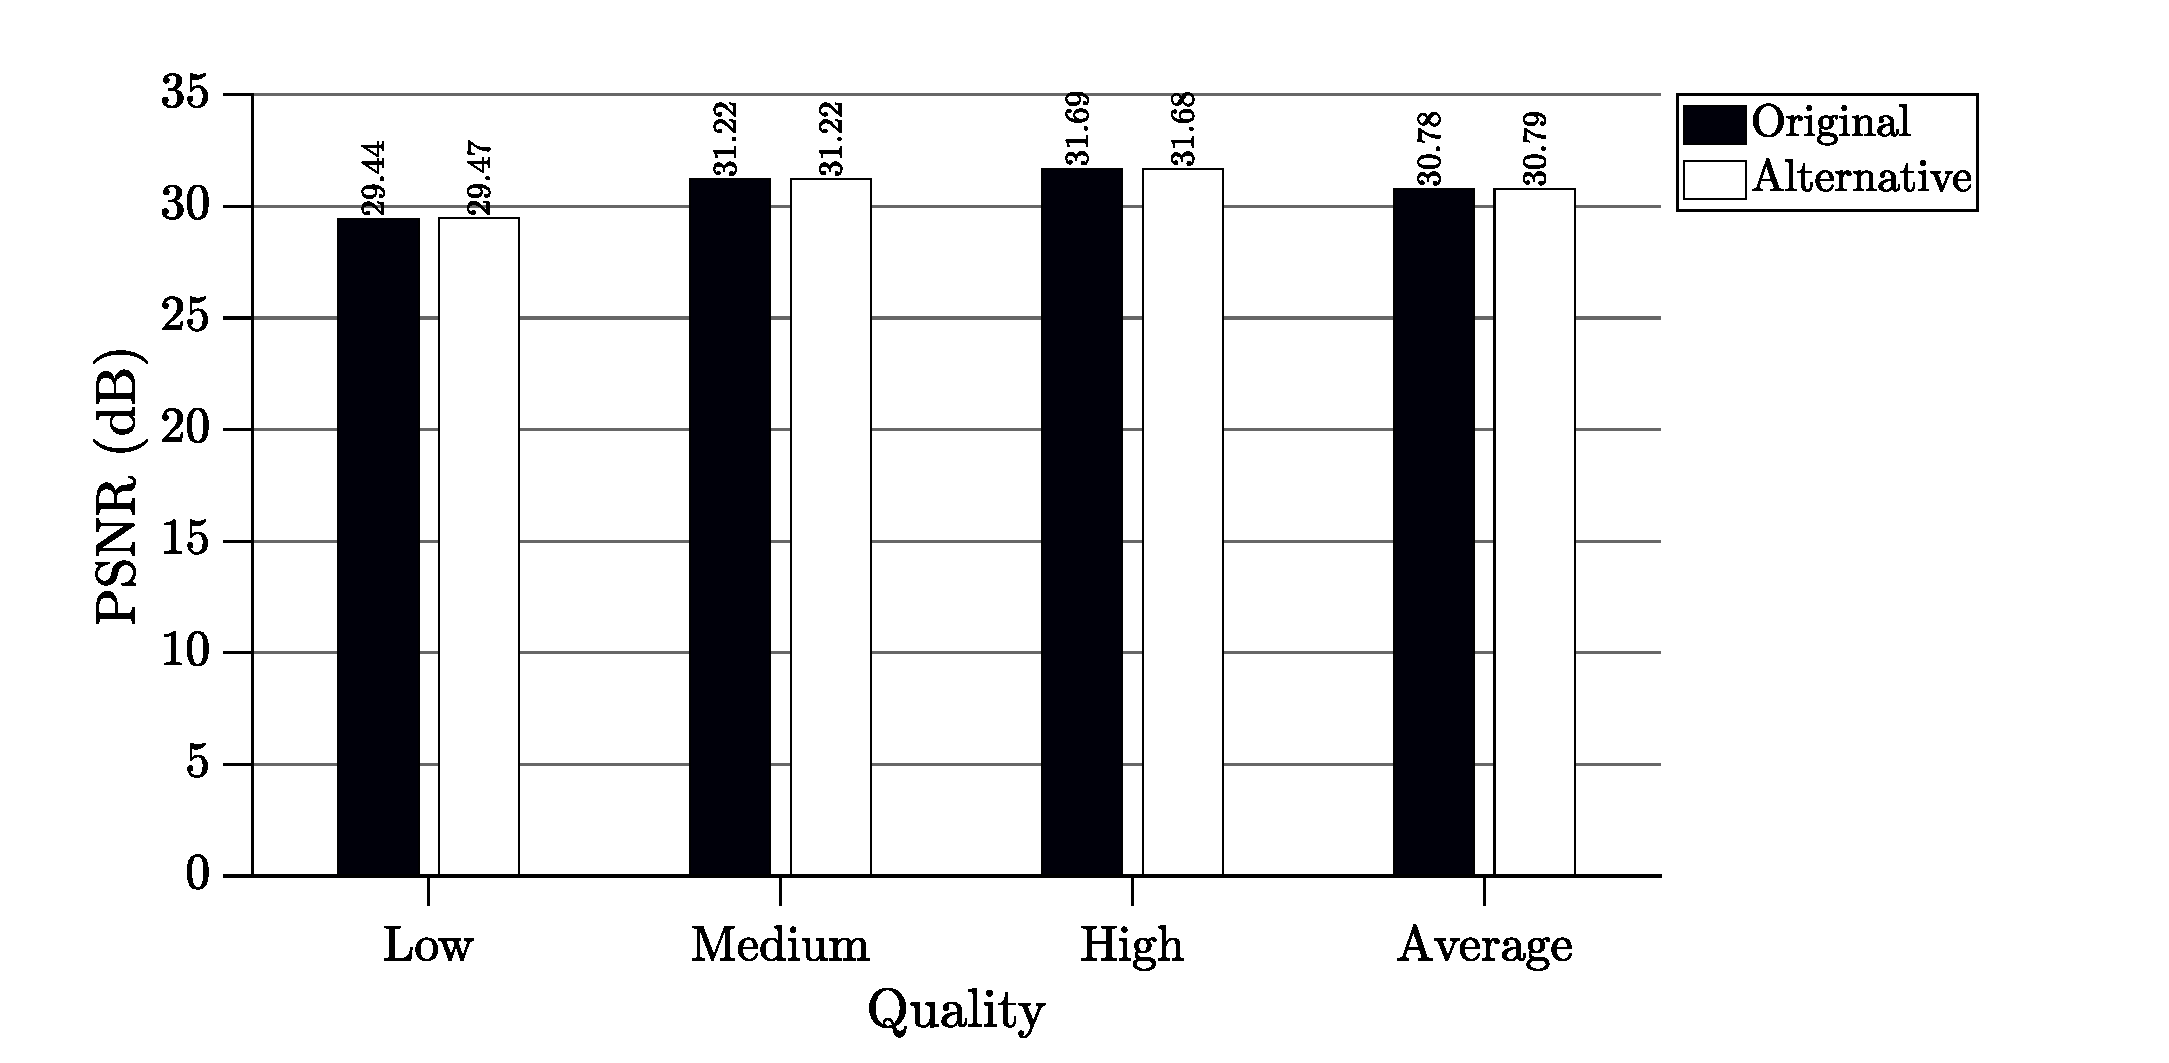
\includegraphics[width=\textwidth]{Sections/4DevelopedArchitecture/Figures/buttmultqual.eps}
    \caption{Obtained quality with original vs alternative \emph{DCT} implementation.}
    \label{fig:buttqual}
\end{figure}

\begin{figure}[!htpb]
    \centering
    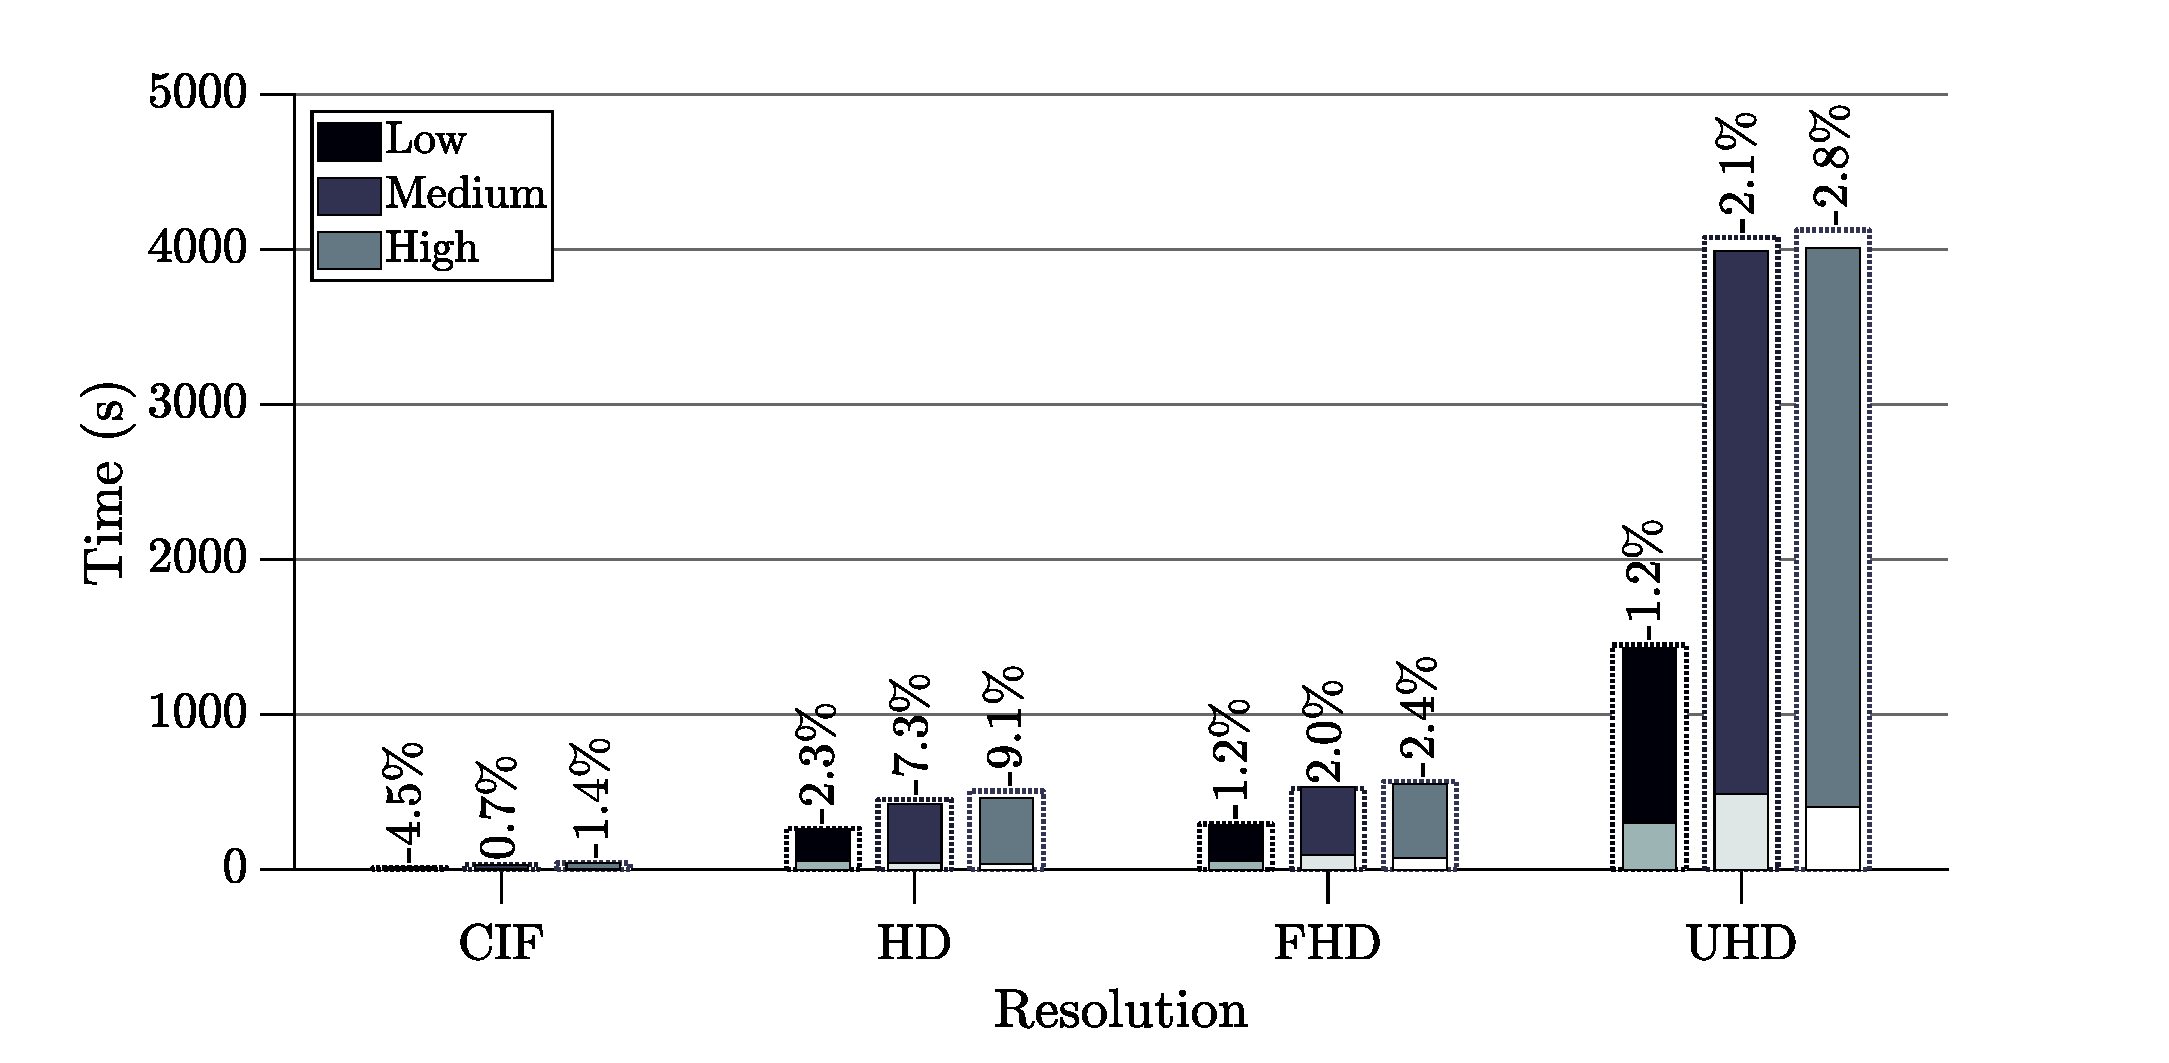
\includegraphics[width=\textwidth]{Sections/4DevelopedArchitecture/Figures/buttmulttime.eps}
    \caption{Encoding time with original vs alternative \emph{DCT} implementation.}
    \label{fig:butttime}
\end{figure}

As shown, with the performed changes, the encoding time was, in average, reduced by $2.9\%$ for all quality objectives, while maintaining the output PSNR, making this a suitable \emph{DCT} implementation for an \emph{AV1} encoder. Although the performance improvement is rather diminishing once considered the full encoding cycle, it is a step toward a possible realtime encoding implementation.

However, the full impact of the applied changes can only be verified on a hardware implementation. With the reduction of the cosine approximations, the memory used in the developed \emph{DCT}s is highly reduced. Considering $M_{\texttt{cospi}}$ as the number of bytes ($B$) used for storing the original cosine approximation vector,

\begin{equation}
    M_{\texttt{cospi}} = \frac{64\cdot (10+11+12+13+14+15+16)}{8} = 728\, B
\end{equation}
On the other hand, with the new implementation, only $64 \, B$  would be needed to store these approximations, corresponding to an $81\%$ reduction.

Nonetheless, both \emph{libaom}'s version and the developed could heavily benefit from parallelization, as is described in the following section.

%%%%%%%%%%%%%%%%%%%%%%%%%%%%%%%%%%%%%%%%%%%%%%%%%%%%%%%%%%%%%%%%%%%%%%%%%%%%%%
\section{Hardware Implementations}

On the subject of hardware prototyping, \glspl{fpga} have gained massive popularity within developers, both because of its applicability, as well as ease of use. Additionally, in recent years, there have been major developments in software platforms that allow for the synthesis of FPGA designs as \glspl{asic}, such as \emph{Cadence}'s \emph{Genus} or \emph{Synopsys' Design Compiler} \cite{GenusSynthesisSolution, DesignCompilerGraphical}. 

This way, the chosen platform for the development of the hardware architectures was \emph{Xilinx}'s \emph{Vivado}, due to the wide availability of its FPGAs, as well as for the wide support from its community. For the focus of this work, the target of the designs was \emph{Digillent}'s \emph{Nexys 4 Artix 7 FPGA} \cite{NexysArtix7FPGA}, at $100MHz$ clock. Although this system is not the most adequate if a full encoder integration is desired, it allows to easily test the applicability of the developed architectures. The designs and test benches were described in \gls{vhdl}.

With an efficient algorithm for each of the supported vector sizes, the first objective was to develop a hardware architecture to implement each of the 1D \emph{DCT}s individually, and group them on a single block at a later stage. Two different architectures were developed. The first implements each of the \emph{DCT} blocks individually, while the latter uses sub-blocks of each \emph{DCT}, in order to achieve the final result. These architectures are explained in the following Sections.

With this approach, it was hopped to reach an architecture that englobed all the \emph{DCT} kernels, allowing to easily chose between each of them, depending on the desired choices made in the beginning of the transform stage.

%%%%%%%%%%%%%%%%%%%%%%%%%%%%%%%%%%%%%%%
\subsection{\emph{Individual 1D DCTs} Design}

The hardware implementations followed the same scheme as the corresponding software counterparts. By this it is meant that the flow of the input towards the output is done in individual and sequential stages. The main difference between these implementations is that in hardware, all of the intermediary signals within each stage are calculated in parallel. 

However, in order to achieve an efficient hardware implementation, some additional measures must be taken into account, mainly when considering the multiplication of signals by the cosine coefficients and re-scaling.

Consider an hypothetical operation performed in the software version, where two intermediary signals, \texttt{x1} and \texttt{x2}, get multiplied by some constant, added, and finally rescaled. In $C$, this operation is easily described in a single line of code, as shown in Figure \ref{fig:hardsoft}. However, to perform the same operation on an hardware descriptive language, some additional steps must be taken. The seemingly simple operation done in software must be deconstructed in various sequential steps, controlled by a clock signal. The operation shown in this Figure is repeated throughout the various \emph{DCT} implementations in hardware, making it the key to the development of the parallel architectures.

\begin{figure}[htb]
    \centering
    \begin{tikzpicture}[%
    >={Triangle[length=6pt,angle'=28]},
    start chain=going below,    % General flow is left-to-right
    node distance=5mm and 16mm, % Global setup of box spacing
    every join/.style={norm},   % Default linetype for connecting boxes
    ]

    \tikzset{
    base/.style={draw, on chain, on grid, align=center, minimum height=3.5ex},
    proc/.style={base, rectangle, fill=black!10},
    inout/.style={base,trapezium,trapezium left angle=70,trapezium right angle=-70, fill=black!12},
    term/.style={proc, rounded corners},
    sum/.style={base, circle, inner sep=0pt, radius=0.4cm, fill=black!8},
    % coord node style is used for placing corners of connecting lines
    coord/.style={coordinate, on chain, on grid, node distance=6mm and 40mm},
    % nmark node style is used for coordinate debugging marks% -------------------------------------------------
    % Connector line styles for different parts of the diagram
    norm/.style={ar, draw},
    free/.style={ar, draw, green3},
    cong/.style={ar, draw, red3},
    it/.style={font={\small\itshape}},
    ar/.style={->, line width=0.4mm},
    nar/.style={ar, red!75!black},
    pathcos/.style={font=\small, sloped}
    }

    \begin{scope}        
        \node [inout] (x1) {\texttt{x1}};
        \node [sum, right=of x1, join] (s1) {$\mathbf{\times}$};
        \node [proc, above=1cm of s1] (a) {\texttt{a}};
            \draw[ar] (a) -- (s1);

        \node [inout, below=1cm of x1] (x2) {\texttt{x2}};      
        \node [sum, right=of x2, join] (s2) {$\mathbf{\times}$};
        \node [below=1cm of s2, proc] (b) {\texttt{b}};
            \draw[ar] (b) -- (s2);

        \node [below left=3.5cm and 1cm of x2, align=center, font={\bfseries}] (clk) {Clock\\Signal};
            \draw[thick] ($(clk.east)+(0.5,0)$) -- (x2 |- clk.east) -- ++(0,0.5) coordinate (inReg) -- ++(0.8,0) -- ++(0,-0.5) -- ++(0.8,0) -- ++(0,0.5) coordinate (mult) -- ++(0.8,0) -- ++(0,-0.5) -- ++(0.8,0) -- ++(0,0.5) coordinate (sum) -- ++(0.8,0) -- ++(0,-0.5) -- ++(0.8,0) -- ++(0,0.5) coordinate (shift) -- ++(0.8,0) -- ++(0,-0.5) -- ++(0.8,0) -- ++(0,0.5) coordinate (out) -- ++(0.8,0);
        
        \node[align=center,anchor=north, font={\bfseries\small}, yshift=21mm, draw=darkgray, thin] (lab1) at (mult) {Multiply};
            \draw[dashed] (mult) --(lab1);
        \node[align=center,anchor=north, font={\bfseries\small}, yshift=14mm, draw=darkgray, thin] (lab2) at (sum) {Sum};
            \draw[dashed] (sum) --(lab2);
        \node[align=center,anchor=north, font={\bfseries\small}, yshift=7mm, draw=darkgray, thin] (lab3) at (shift) {Shift};
            \draw[dashed] (shift) --(lab3);

        \path (s1) -- (s2) node[midway, rotate=90] (mid_s) {};
        \node [sum, right=of mid_s] (s3) {$\mathbf{+}$};
            \draw[ar] (s1.east) -- (s3);
            \draw[ar] (s2.east) -- (s3);

        \node[draw, fill=black!10, right=16mm of s3.center, anchor=center] (sh8) {\texttt{>>8}};
            \draw[ar] (s3) -- (sh8);

        \node[inout, right=of sh8, anchor=center] (y) {\texttt{y}};
            \draw[ar] (sh8) -- (y);

        \path (x1) -- (x2) node[midway, rotate=90] (mid_x) {};
        \path (mid_x) -- (y) node[midway, rotate=90] (center) {};        
        \node[above=3cm of center] (eq) {\texttt{y = (a*x1 + b*x2)>>8;}};        
    \end{scope}

    \begin{pgfonlayer}{background}
        \path (clk.west |- a.north)+(-5mm,2mm) node (a11) {};
        \path (y.east |- clk.south)+(20mm,-2mm) node (a21) {};
        \path[fill=black!2,rounded corners, draw=black!50, dashed]
          (a11) rectangle (a21);
        \path (y.east |- a.north)+(20mm,2mm) node (a22) {};
            \path (a21) -- (a22) node[midway, rotate=90, yshift=0.5cm] (mid_right) {\textbf{Hardware}};

        \path (clk.west |- eq.north)+(-5mm,7mm) node (a11) {};
        \path (y.east |- eq.south)+(20mm,-7mm) node (a21) {};
        \path[fill=black!2,rounded corners, draw=black!50, dashed]
          (a11) rectangle (a21);
        \path (y.east |- eq.north)+(20mm,7mm) node (a22) {};
            \path (a21) -- (a22) node[midway, rotate=90, yshift=0.5cm] (mid_right) {\textbf{Software}};
    \end{pgfonlayer}
\end{tikzpicture}
    \caption{Comparison between software and hardware implementation of multiplication, sum and re-scaling.}
    \label{fig:hardsoft}
\end{figure}

Due to advances in \emph{VHDL} compilers and supporting libraries, both multiplication, shifts and additions are easily described, on a similar manner to a higher level language. Although on previous generations there would be some added benefits of implementing a multiplication by shifting and adding an input, as shown in Equation \ref{eq:multshift}, the improvements done in most recent years allow for similar architectures to be implemented, with less effort.

\begin{equation} \label{eq:multshift}
    \texttt{15 * x1} \equiv \texttt{(x1<<3) + (x1<<2) + (x1<<1) + x1}
\end{equation}

Taking these measures into consideration, the development of the 1D transforms becomes similar to all vector sizes. The software implementations are composed of alternating stages of simple summing operations, with more complex multiplying, sum and shift cycles. Therefore, the hardware counterparts are composed of three different blocks:

\begin{itemize}
    \item \emph{Summing Stages} where the inputs get added according to the previously shown butterfly schemes;
    \item \emph{Multiplier Stages}, which multiply the necessary inputs by the corresponding cosine coefficients;
    \item \emph{Shift Stages} that rescale the coefficients.
\end{itemize} 

Although these blocks are unique between transform sizes, and even within the same \emph{DCT}, the operations performed within are similar between all the vector sizes.

In order to ensure the correct pipelining of the \emph{Transform} process, each stage is controlled by an \emph{enable} flag, \texttt{en}, which signals the start of the block's process. Once it is concluded, the block outputs an indicator, \texttt{valOut}, that acts as the enable for the following stage, creating a daisy chain of stages. The last stage's \texttt{valOut} acts as the indication of the conclusion of the \emph{Transform} operation.

All blocks are controlled by the same \emph{clock} and \emph{reset} signals. The first triggers the internal processes on its ascending flank. The latter signals all internal registers to be put to 0 (its initial stage).

A simplified version of \textbf{DCT4}'s hardware implementation is represented in Figure \ref{fig:harddct4v1}. In here, the direction of the arrow represents if the corresponding signal is a \emph{input} or \emph{output}. The numbering of the output coefficients is done accordingly to the software implementation.

\begin{figure}[!htbp]
    \centering
    \begin{tikzpicture}[%
    >={Triangle[length=6pt,angle'=28]},
    start chain=going below ,    % General flow is left-to-right
    node distance=5mm and 20mm, % Global setup of box spacing
    every join/.style={norm},   % Default linetype for connecting boxes
    scale=0.8, 
    every node/.style={transform shape}
    ]

  \tikzset{
    base/.style={draw, on chain, on grid, align=center, minimum height=3.5ex},
    reg/.style={base, rectangle, minimum width=2.5em, minimum height=2em,fill=black!15},
    proc/.style={base, rectangle, minimum width=4em, minimum height=8em, fill=black!15},
    inout/.style={base,trapezium,trapezium left angle=70,trapezium right angle=-70, fill=blue!12},
    term/.style={proc, rounded corners},
    sum/.style={base, circle, inner sep=0pt, radius=0.4cm, fill=black!15},
    % coord node style is used for placing corners of connecting lines
    coord/.style={coordinate, on chain, on grid, node distance=6mm and 40mm},
    % nmark node style is used for coordinate debugging marks% -------------------------------------------------
    % Connector line styles for different parts of the diagram
    norm/.style={ar32, draw},
    free/.style={ar32, draw, green3},
    cong/.style={ar32, draw, red3},
    it/.style={font={\small\itshape}},
    nar/.style={ar32, red!75!black},
    ar32/.style={->, line width=0.8mm},   
    b32/.style={line width=0.8mm},    
    ar1/.style={->, line width=0.4mm}  
  }    

  \begin{scope}[y=-1cm]
    \begin{scope}
      %\draw[step=1cm, very thin, lightgray] (0,0) grid (14,21);
      
      %% Inputs
      \draw [black,very thick] (1,0) circle (1mm) node [right, rotate=90, xshift=1mm] {\texttt{Clock}};
        %\draw [ar32] (1,0.1) |- (5,19.5-1);
        \draw [ar1] (1,0.1) |- (5,15.5-1);
        \draw [ar1] (1,0.1) |- (5,11.5-1);
        \draw [ar1] (1,0.1) |- (5,7.5-1);
        \draw [ar1] (1,0.1) |- (5,3.5-1);
      \draw [black,very thick] (2,0) circle (1mm) node [right, rotate=90, xshift=1mm] {\texttt{Reset}};
        %\draw [ar32] (2,0.1) |- (5,19.5-1.5);
        \draw [ar1] (2,0.1) |- (5,15.5-1.5);
        \draw [ar1] (2,0.1) |- (5,11.5-1.5);
        \draw [ar1] (2,0.1) |- (5,7.5-1.5);
        \draw [ar1] (2,0.1) |- (5,3.5-1.5);
      \draw [black,very thick] (3,0) circle (1mm) node [right, rotate=90, xshift=1mm] {\texttt{Enable}};
        \draw [ar1] (3,0.1) |- (5,1.5);
      \foreach \x in {0,...,3}
        \draw [black,very thick] (6+2*\x,0) circle (1mm) node [right, rotate=90, xshift=1mm] (dIn\x) {\texttt{dataIn\x}};      

      %% In Register
      \node (inReg) at (5,2-1) [draw,thick,minimum width=8cm,minimum height=3cm, rounded corners, anchor=north west, fill=black!8, font={\large}] {\textbf{Stage 1: Sum}};
      \node (enInReg) at (5,2.5-1) [right, font={\small}] {\texttt{en}};
      \node (resInReg) at (5,3-1) [right, font={\small}] {\texttt{res}};
      \node (clkInReg) at (5,3.5-1) [right, font={\small}] {\texttt{clk}};
      \node (valoutInReg) at (5,4.5-1) [right, font={\small}] {\texttt{valOut}};
        \draw [ar1] (5,4.5-1) -- ++(-1,0) |- (5,6.5-1);

      %% Stage 1 Sum
      \node (St1) at (5,6-1) [draw,thick,minimum width=8cm,minimum height=3cm, rounded corners, anchor=north west, fill=black!8, font={\large}] {\textbf{Stage 2: Multiplier}};
      \node (enSt1) at (5,6.5-1) [right, font={\small}] {\texttt{en}};
      \node (resSt1) at (5,7-1) [right, font={\small}] {\texttt{res}};
      \node (clkSt1) at (5,7.5-1) [right, font={\small}] {\texttt{clk}};
      \node (valoutSt1) at (5,8.5-1) [right, font={\small}] {\texttt{valOut}};
        \draw [ar1] (5,8.5-1) -- ++(-1,0) |- (5,10.5-1);

      %% Stage 2 Mult
      \node (St2M) at (5,10-1) [draw,thick,minimum width=8cm,minimum height=3cm, rounded corners, anchor=north west, fill=black!8, font={\large}] {\textbf{Stage 2: Sum}};
      \node (enSt2M) at (5,10.5-1) [right, font={\small}] {\texttt{en}};
      \node (resSt2M) at (5,11-1) [right, font={\small}] {\texttt{res}};
      \node (clkSt2M) at (5,11.5-1) [right, font={\small}] {\texttt{clk}};
      \node (valoutSt2M) at (5,12.5-1) [right, font={\small}] {\texttt{valOut}};
        \draw [ar1] (5,12.5-1) -- ++(-1,0) |- (5,14.5-1);
      
      %% Stage 2 Add
      \node (St2A) at (5,14-1) [draw,thick,minimum width=8cm,minimum height=3cm, rounded corners, anchor=north west, fill=black!8, font={\large}] {\textbf{Stage 2: Shift}};
      \node (enSt2A) at (5,14.5-1) [right, font={\small}] {\texttt{en}};
      \node (resSt2A) at (5,15-1) [right, font={\small}] {\texttt{res}};
      \node (clkSt2A) at (5,15.5-1) [right, font={\small}] {\texttt{clk}};
      \node (valoutSt2A) at (5,16.5-1) [right, font={\small}] {\texttt{valOut}}; 
        \draw [ar1] (5,15.5) -| (2,16.5);
        \draw [line width=0.4mm] (2,16.5) -- ++(0,0.4);

      
      %%% Stage 2 Shift
      %\node (St2S) at (5,18-1) [draw,thick,minimum width=8cm,minimum height=3cm, rounded corners, anchor=north west, fill=black!8, font={\large}] {\textbf{Stage 2: Shift}};
      %\node (enSt2S) at (5,18.5-1) [right, font={\small}] {\texttt{en}};
      %\node (resSt2S) at (5,19-1) [right, font={\small}] {\texttt{res}};
      %\node (clkSt2S) at (5,19.5-1) [right, font={\small}] {\texttt{clk}};
      %\node (valoutSt2S) at (5,20.5-1) [right, font={\small}] {\texttt{valOut}};  
      %  \draw [ar32] (5,20.5-1) -| (2,20.5); 
      %  \draw[line width=0.4mm] (2,20.5) -- ++(0, -0.4cm);
      
      %% Outputs
      \draw [black,very thick] (2,17) circle (1mm) node [left, rotate=90, xshift=-1mm] {\texttt{validOut}};
      
      \draw [black,very thick] (6,17) circle (1mm) node [left, rotate=90, xshift=-1mm] (dOut0) {\texttt{dataOut0}};
      \draw [black,very thick] (6+2*1,17) circle (1mm) node [left, rotate=90, xshift=-1mm] (dOut2) {\texttt{dataOut2}};
      \draw [black,very thick] (6+2*2,17) circle (1mm) node [left, rotate=90, xshift=-1mm] (dOut1) {\texttt{dataOut1}};
      \draw [black,very thick] (6+2*3,17) circle (1mm) node [left, rotate=90, xshift=-1mm] (dOut3) {\texttt{dataOut3}};

      \foreach \x in {0,...,3} {
        \draw[ar32] (6+2*\x,-1mm) -- ++(0, -0.9cm);
        \draw[ar32] (6+2*\x,4) -- ++(0, -1cm);
        \draw[ar32] (6+2*\x,8) -- ++(0, -1cm);
        \draw[ar32] (6+2*\x,12) -- ++(0, -1cm);
        \draw[ar32] (6+2*\x,16) -- ++(0, -0.5cm);
        %\draw[ar32] (6+2*\x,20) -- ++(0, -0.5cm);
        \draw[b32] (6+2*\x,16.5) -- ++(0, -0.4cm);
      }
    \end{scope}
    \begin{pgfonlayer}{background}
      % Left-top corner of the background rectangle
      \node (a11) at (0,0.5) {};
      % Right-bottom corner of the background rectanle
      \node (a21) at (13.5,16.5) {};
      % Draw the background
      \path[fill=black!3,rounded corners, draw, very thick]
        (a11) rectangle (a21);
      \node (a31) at (1.5,16.5) {};
      \path (a11) -- (a31) node[midway, rotate=90, yshift=1.3cm, font={\huge}] (mid_right) {\textbf{DCT4}};
    \end{pgfonlayer}
  \end{scope}
\end{tikzpicture}
    \caption{1D \textbf{DCT4} hardware implementation.}
    \label{fig:harddct4v1}
\end{figure}

To simplify the development of the hardware architectures, all signals and internal registers are represented, as this measure allows to easily interconnect the developed modules. Nonetheless, all modules are configurable through the modification of a \gls{genmap}.

On a post-prototyping stage, to achieve an optimal utilization of resources, both inputs, outputs and internal signals should be shortened to the minimum length.

As a final measure to simplify the development process, the \emph{kernels} are implemented using the smaller sizes as a constituting block. As shown in Wen-Hsiung Chen's work \cite{wen-hsiungchenFastComputationalAlgorithm1977}, all transform sizes greater than $4$ englobe the same sequence of operations as the smaller counterparts, on one subset of its intermediary coefficients. This way, each of the smaller \emph{1D-DCT} blocks may be inserted into the size immediately above it.

As an example, \textbf{DCT8}'s hardware implementation is represented in Figure \ref{fig:harddct8v1}. There, it is observable that the architecture is similarly composed of the same blocks as the previous implementation. However, after the first summing stage, the first four intermediary coefficients are input into \textbf{DCT4}. 

\begin{figure}[!htbp]
    \centering
    \begin{tikzpicture}[%
    >={Triangle[length=6pt,angle'=28]},
    start chain=going below ,    % General flow is left-to-right
    node distance=5mm and 20mm, % Global setup of box spacing
    every join/.style={norm},   % Default linetype for connecting boxes
    scale=0.8, 
    every node/.style={transform shape},
    circuit logic US, every circuit symbol/.style={thick}
    ]

  \tikzset{
    base/.style={draw, on chain, on grid, align=center, minimum height=3.5ex},
    reg/.style={base, rectangle, minimum width=2.5em, minimum height=2em,fill=black!15},
    proc/.style={base, rectangle, minimum width=4em, minimum height=8em, fill=black!15},
    inout/.style={base,trapezium,trapezium left angle=70,trapezium right angle=-70, fill=blue!12},
    term/.style={proc, rounded corners},
    sum/.style={base, circle, inner sep=0pt, radius=0.4cm, fill=black!15},
    % coord node style is used for placing corners of connecting lines
    coord/.style={coordinate, on chain, on grid, node distance=6mm and 40mm},
    % nmark node style is used for coordinate debugging marks% -------------------------------------------------
    % Connector line styles for different parts of the diagram
    norm/.style={ar32, draw},
    free/.style={ar32, draw, green3},
    cong/.style={ar32, draw, red3},
    it/.style={font={\small\itshape}},
    nar/.style={ar32, red!75!black},
    ar32/.style={->, line width=0.8mm},   
    b32/.style={line width=0.8mm},    
    ar1/.style={->, line width=0.4mm}
  }    

  \begin{scope}[y=-1cm]
    \begin{scope}
      %\draw[step=1cm, very thin, lightgray] (0,0) grid (14,30);
      
      %% Inputs
      \draw [black,very thick] (1,4) circle (1mm) node [right, rotate=90, xshift=1mm] {\texttt{Clock}};
        \draw [ar1] (1,4.1) |- (9.5,16);
        \draw [ar1] (1,4.1) |- (4,10.5);
        \draw [ar1] (1,4.1) -- (1,8.6) -- ++(7.7,0) |- (9.5,11.5-1);
        \draw [ar1] (1,4.1) |- (4,7.5-1);
        %\draw [ar32] (1,4.1) |- (4,3.5-1);
      \draw [black,very thick] (2,4) circle (1mm) node [right, rotate=90, xshift=1mm] {\texttt{Reset}};
        \draw [ar1] (2,4.1) |- (9.5,15.5);
        \draw [ar1] (2,4.1) |- (4,10);
        \draw [ar1] (2,4.1) -- (2,8.4) -- ++(6.9,0) |- (9.5,11-1);
        \draw [ar1] (2,4.1) |- (4,6);
        %\draw [ar32] (2,4.1) |- (4,3.5-1);
      \draw [black,very thick] (3,4) circle (1mm) node [right, rotate=90, xshift=1mm] {\texttt{Enable}};
        \draw [ar1] (3,4.1) |- (4,5.5);
      \foreach \x in {0,...,3}
        \draw [black,very thick] (5+\x,4) circle (1mm) node [right, rotate=90, xshift=1mm] (dIn\x) {\texttt{dataIn\x}};
      \foreach \x in {4,...,7}
        \draw [black,very thick] (6+\x,4) circle (1mm) node [right, rotate=90, xshift=1mm] (dIn\x) {\texttt{dataIn\x}};

      %% In Register
      %\node (inReg) at (5-1,2-1) [draw,thick,minimum width=10cm,minimum height=3cm, rounded corners, anchor=north west, fill=black!8, font={\large}] {\textbf{Input Register}};
      %\node (enInReg) at (5-1,2.5-1) [right, font={\small}] {\texttt{en}};
      %\node (resInReg) at (5-1,3-1) [right, font={\small}] {\texttt{res}};
      %\node (clkInReg) at (5-1,3.5-1) [right, font={\small}] {\texttt{clk}};
      %\node (valoutInReg) at (5-1,4.5-1) [right, font={\small}] {\texttt{valOut}};
      %  \draw [ar32] (5-1,4.5-1) -- ++(-1,0) |- (5-1,6.5-1);

      %% Stage 1 Sum
      \node (St1) at (5-1,6-1) [draw,thick,minimum width=10cm,minimum height=3cm, rounded corners, anchor=north west, fill=black!8, font={\large}] {\textbf{Stage 1: Sum}};
      \node (enSt1) at (5-1,6.5-1) [right, font={\small}] {\texttt{en}};
      \node (resSt1) at (5-1,7-1) [right, font={\small}] {\texttt{res}};
      \node (clkSt1) at (5-1,7.5-1) [right, font={\small}] {\texttt{clk}};
      \node (valoutSt1) at (5-1,8.5-1) [right, font={\small}] {\texttt{valOut}};
        \draw [ar1] (5-1,8.5-1) -- ++(-1,0) |- (5-1,10.5-1);
        \draw [ar1] (5-1,8.5-1) -- ++(-1,0) -- ++(0,0.7) -- ++(6.1,0) |- (9.5,10.5-1);

      %% DCT4
      \node (DCT4) at (4,9) [draw,thick,minimum width=4.5cm,minimum height=3cm, rounded corners, anchor=north west, fill=black!12, font={\large\bfseries}, align=center] {DCT4};
      \node (enSt2M) at (5-1,10.5-1) [right, font={\small}] {\texttt{en}};
      \node (resSt2M) at (5-1,11-1) [right, font={\small}] {\texttt{res}};
      \node (clkSt2M) at (5-1,11.5-1) [right, font={\small}] {\texttt{clk}};
      \node (valoutDCT4) at (5-1,12.5-1) [right, font={\small}] {\texttt{valOut}};
    
      %% Stage 2 Mult
      \node (St2M) at (9.5,9) [draw,thick,minimum width=4.5cm,minimum height=3cm, rounded corners, anchor=north west, fill=black!8, font={\large\bfseries}, align=center] {Stage 2:\\Multiplier};
      \node (enSt2M) at (9.5,10.5-1) [right, font={\small}] {\texttt{en}};
      \node (resSt2M) at (9.5,11-1) [right, font={\small}] {\texttt{res}};
      \node (clkSt2M) at (9.5,11.5-1) [right, font={\small}] {\texttt{clk}};
      \node (valoutSt2M) at (9.5,12.5-1) [right, font={\small}] {\texttt{valOut}};
        \draw [ar1] (9.5,12.5-1) -- ++(-0.5,0) -- ++(0,1.5) coordinate (etc);
    
      \foreach \x in {0,...,4}
        \node at (etc) [left, rotate=90, xshift=-1mm, yshift=-\x cm, font={\bfseries}] {...};

      %% Stage 4 Shift
      \foreach \x in {0,...,3}
        \draw [ar32] (10+\x,14) -- ++(0,0.5);
      \draw [ar1] (9,14) |- (9.5,15);
      \node (St4S) at (9.5,14.5) [draw,thick,minimum width=4.5cm,minimum height=3cm, rounded corners, anchor=north west, fill=black!8, font={\large\bfseries}, align=center] {Stage 4:\\Shift};
      \node (enSt2S) at (9.5,15) [right, font={\small}] {\texttt{en}};
      \node (resSt2S) at (9.5,15.5) [right, font={\small}] {\texttt{res}};
      \node (clkSt2S) at (9.5,16) [right, font={\small}] {\texttt{clk}};
      \node (valoutSt2S) at (9.5,17) [right, font={\small}] {\texttt{valOut}}; 
        %\draw [ar32] (9.5,20.5-1) -| (2-1,20.5); 
        
        \node[and gate,inputs={nnnn}, point down] (and1) at (1,18)    {};
            \draw[ar1] (valoutSt2S) -| (and1.input 1);
            \draw[ar1] (valoutDCT4) -| (and1.input 4);
            \draw[ar1] (and1.output) -- (1, 19.5);
            \draw[line width=0.4mm] (1, 19.5) -- ++(0, 0.4);

      %% Outputs
      \draw [black,very thick] (2-1,20) circle (1mm) node [left, rotate=90, xshift=-1mm] {\texttt{validOut}};
      \draw [black,very thick] (5+0,20) circle (1mm) node [left, rotate=90, xshift=-1mm] (dOut0) {\texttt{dataOut0}};
      \draw [black,very thick] (5+1,20) circle (1mm) node [left, rotate=90, xshift=-1mm] (dOut4) {\texttt{dataOut4}};
      \draw [black,very thick] (5+2,20) circle (1mm) node [left, rotate=90, xshift=-1mm] (dOut2) {\texttt{dataOut2}};
      \draw [black,very thick] (5+3,20) circle (1mm) node [left, rotate=90, xshift=-1mm] (dOut6) {\texttt{dataOut6}};
      
      \draw [black,very thick] (6+4,20) circle (1mm) node [left, rotate=90, xshift=-1mm] (dOut1) {\texttt{dataOut1}};
      \draw [black,very thick] (6+5,20) circle (1mm) node [left, rotate=90, xshift=-1mm] (dOut5) {\texttt{dataOut5}};
      \draw [black,very thick] (6+6,20) circle (1mm) node [left, rotate=90, xshift=-1mm] (dOut3) {\texttt{dataOut3}};
      \draw [black,very thick] (6+7,20) circle (1mm) node [left, rotate=90, xshift=-1mm] (dOut7) {\texttt{dataOut7}};

      \foreach \x in {0,...,3} {
        %\draw[ar32] (5+\x,-1mm) -- ++(0, -0.9cm);
        \draw[ar32] (5+\x,4.1) -- ++(0, -0.9cm);
        \draw[ar32] (5+\x,8) -- ++(0, -1cm);
        \draw[ar32] (5+\x,12) -- ++(0, -7.5cm);       
        \draw[b32] (5+\x,19.5) -- ++(0, -0.4cm);
      }
      \foreach \x in {4,...,7} {
        %\draw[ar32] (6+\x,-1mm) -- ++(0, -0.9cm);
        \draw[ar32] (6+\x,4.1) -- ++(0, -0.9cm);
        \draw[ar32] (6+\x,8) -- ++(0, -1cm);
        \draw[ar32] (6+\x,12) -- ++(0, -1cm);
        \draw[ar32] (6+\x,17.5) -- ++(0, -2cm);
        \draw[b32] (6+\x,19.5) -- ++(0, -0.4cm);
      }
    \end{scope}
    \begin{pgfonlayer}{background}
      % Left-top corner of the background rectangle
      \node (a11) at (0,4.5) {};
      % Right-bottom corner of the background rectanle
      \node (a21) at (14.5,19.5) {};
      % Draw the background
      \path[fill=black!3,rounded corners, draw, very thick]
        (a11) rectangle (a21);
      \node (a31) at (1.5,19.5) {};
      \path (a11) -- (a31) node[midway, rotate=90, yshift=1.3cm, font={\huge}] (mid_right) {\textbf{DCT8}};
    \end{pgfonlayer}
  \end{scope}
\end{tikzpicture}
    \caption{Simplified 1D \textbf{DCT8} hardware implementation, with inclusion of \textbf{DCT4}.}
    \label{fig:harddct8v1}
\end{figure}

In the same manner, \textbf{DCT16} includes \textbf{DCT8}, which, as shown, also includes the four input version. This approach causes the smaller blocks to be repeated throughout the various larger architectures, making this approach highly inefficient from the chip's utilization standpoint.

Nonetheless, in order to draw conclusions as to the correct functioning of the internal stages, as well as to see possible gains from the following implementations, the architecture from Figure \ref{fig:fullv1} was developed.

\begin{figure}[!htbp]
    \centering
    \begin{tikzpicture}[%
    >={Triangle[length=6pt,angle'=28]},
    start chain=going below ,    % General flow is left-to-right
    node distance=5mm and 20mm, % Global setup of box spacing
    every join/.style={norm},   % Default linetype for connecting boxes
    scale=0.8, 
    every node/.style={transform shape},
    circuit logic US, every circuit symbol/.style={thick}
    ]

  \tikzset{
    base/.style={draw, on chain, on grid, align=center, minimum height=3.5ex},
    reg/.style={base, rectangle, minimum width=2.5em, minimum height=2em,fill=black!15},
    proc/.style={base, rectangle, minimum width=4em, minimum height=8em, fill=black!15},
    inout/.style={base,trapezium,trapezium left angle=70,trapezium right angle=-70, fill=blue!12},
    term/.style={proc, rounded corners},
    sum/.style={base, circle, inner sep=0pt, radius=0.4cm, fill=black!15},
    % coord node style is used for placing corners of connecting lines
    coord/.style={coordinate, on chain, on grid, node distance=6mm and 40mm},
    % nmark node style is used for coordinate debugging marks% -------------------------------------------------
    % Connector line styles for different parts of the diagram
    norm/.style={aar, draw},
    ar32/.style={->, line width=0.8mm},   
    b32/.style={line width=0.8mm},    
    ar1/.style={->, line width=0.4mm}  
  }    

  \begin{scope}[y=-1cm]
    \begin{scope}
      %\draw[step=1cm, very thin, lightgray] (0,0) grid (14,20);            
        
        %% Inputs/Outputs

        % IN/OUT 0-3
        \foreach \x in {0,...,3}
            \draw [black,very thick] (0,1+0.5*\x) circle (1mm) node [left, xshift=-1mm] (dIn\x) {\texttt{dataIn\x}};      
        \node at (0,3) [anchor=east, rotate=90, font={\bfseries}] {...};
            
            \foreach \x in {0,...,3} {
                \draw[ar32] (0.1,1+0.5*\x) -- ++(1.9,0);                
            }
            \draw[ar32] (1,1) |- (2,4.5);
                \node at (1.5,5) [anchor=east, rotate=90, font={\bfseries}] {...};
            \draw[ar32] (1,4.5) |- (2,8);
                \node at (1.5,8.5) [anchor=east, rotate=90, font={\bfseries}] {...};
            \draw[ar32] (1,8) |- (2,11.5);
                \node at (1.5,12) [anchor=east, rotate=90, font={\bfseries}] {...};
            \draw[ar32] (1,11.5) |- (2,15);
                \node at (1.5,15.5) [anchor=east, rotate=90, font={\bfseries}] {...};

            \draw[ar32] (6.5,1) node [above, font={\small\ttfamily}, align=center, xshift=0.75cm] {DCT4o0} -- ++(1.5,0);
            \node at (7,1) [anchor=east, rotate=90, font={\bfseries}] {...};
            \draw[ar32] (6.5,2) node [above, font={\small\ttfamily}, align=center, xshift=0.75cm] {DCT4o3} -- ++(1.5,0);
            \draw[ar1] (6.5,2.5) node [above, font={\small\ttfamily}, align=center, xshift=0.75cm] {DCT4vo} -- ++(1.5,0);


        % IN 7/DCT8
        \draw [black,very thick] (0,6) circle (1mm) node [left, xshift=-1mm] (dIn7) {\texttt{dataIn7}};      
            \node at (0.25,6.5) [anchor=east, rotate=90, font={\bfseries}] {...};

                \draw[ar32] (0.1,6) -- ++(1.9,0);
                \draw[ar32] (0.5,6) -- ++(0,0.5);

                \draw[ar32] (6.5,4.5) node [above, font={\small\ttfamily}, align=center, xshift=0.75cm] {DCT8o0} -- ++(1.5,0);
                \node at (7,4.5) [anchor=east, rotate=90, font={\bfseries}] {...};
                \draw[ar32] (6.5,5.5) node [above, font={\small\ttfamily}, align=center, xshift=0.75cm] {DCT8o7} -- ++(1.5,0);
                \draw[ar1] (6.5,6) node [above, font={\small\ttfamily}, align=center, xshift=0.75cm] {DCT8vo} -- ++(1.5,0);

        % IN 15/DCT16
        \draw [black,very thick] (0,9.5) circle (1mm) node [left, xshift=-1mm] (dIn15) {\texttt{dataIn15}};      
            \node at (0.25,10) [anchor=east, rotate=90, font={\bfseries}] {...};

                \draw[ar32] (0.1,9.5) -- ++(1.9,0);
                \draw[ar32] (0.5,9.5) -- ++(0,0.5);

                \draw[ar32] (6.5,8) node [above, font={\small\ttfamily}, align=center, xshift=0.75cm] {DCT16o0} -- ++(1.5,0);
                \node at (7,8) [anchor=east, rotate=90, font={\bfseries}] {...};
                \draw[ar32] (6.5,9) node [above, font={\small\ttfamily}, align=center, xshift=0.75cm] {DCT16o15} -- ++(1.5,0);
                \draw[ar1] (6.5,9.5) node [above, font={\small\ttfamily}, align=center, xshift=0.75cm] {DCT16vo} -- ++(1.5,0);

        % IN 31/DCT32
        \draw [black,very thick] (0,13) circle (1mm) node [left, xshift=-1mm] (dIn31) {\texttt{dataIn31}};      
            \node at (0.25,13.5) [anchor=east, rotate=90, font={\bfseries}] {...};

                \draw[ar32] (0.1,13) -- ++(1.9,0);
                \draw[ar32] (0.5,13) -- ++(0,0.5);

                \draw[ar32] (6.5,11.5) node [above, font={\small\ttfamily}, align=center, xshift=0.75cm] {DCT32o0} -- ++(1.5,0);
                \node at (7,11.5) [anchor=east, rotate=90, font={\bfseries}] {...};
                \draw[ar32] (6.5,12.5) node [above, font={\small\ttfamily}, align=center, xshift=0.75cm] {DCT32o31} -- ++(1.5,0);
                \draw[ar1] (6.5,13) node [above, font={\small\ttfamily}, align=center, xshift=0.75cm] {DCT32vo} -- ++(1.5,0);

        % IN 63/DCT64
        \draw [black,very thick] (0,16.5) circle (1mm) node [left, xshift=-1mm] (dIn63) {\texttt{dataIn63}};      

                \draw[ar32] (0.1,16.5) -- ++(1.9,0);
            
                \draw[ar32] (6.5,15) node [above, font={\small\ttfamily}, align=center, xshift=0.75cm] {DCT64o0} -- ++(1.5,0);
                \node at (7,15) [anchor=east, rotate=90, font={\bfseries}] {...};
                \draw[ar32] (6.5,16) node [above, font={\small\ttfamily}, align=center, xshift=0.75cm] {DCT64o63} -- ++(1.5,0);
                \draw[ar1] (6.5,16.5) node [above, font={\small\ttfamily}, align=center, xshift=0.75cm] {DCT64vo} -- ++(1.5,0);

        % Clock
        \draw [black,very thick] (0,18) circle (1mm) node [left, xshift=-1mm] (clk) {\texttt{Clock}};            
            \draw[ar1] (0.1,18) -- (2.2,18) -- (2.2,3.4) -| (3,3);
            \draw[ar1] (2.2,6.9) -| (3,6.5);
            \draw[ar1] (2.2,10.4) -| (3,10);
            \draw[ar1] (2.2,13.9) -| (3,13.5);
            \draw[ar1] (2.2,17.4) -| (3,17);
            \draw[ar1] (2.2,18) -- (8,18);
        
        % Reset
        \draw [black,very thick] (0,18.5) circle (1mm) node [left, xshift=-1mm] (res) {\texttt{Reset}};
            \draw[ar1] (0.1,18.5) -- (2.4,18.5) -- (2.4,3.6) -| (3.5,3);
            \draw[ar1] (2.4,7.1) -| (3.5,6.5);
            \draw[ar1] (2.4,10.6) -| (3.5,10);
            \draw[ar1] (2.4,14.1) -| (3.5,13.5);
            \draw[ar1] (2.4,17.6) -| (3.5,17);
            \draw[ar1] (2.4,18.5) -- (8,18.5);

        % Enable
        \draw [black,very thick] (0,19) circle (1mm) node [left, xshift=-1mm] (enin) {\texttt{Enable}};
            \draw[ar1] (0.1,19) -- (2.6,19) -- (2.6,3.8) -| (4,3);
            \draw[ar1] (2.6,7.3) -| (4,6.5);
            \draw[ar1] (2.6,10.8) -| (4,10);
            \draw[ar1] (2.6,14.3) -| (4,13.5);
            \draw[ar1] (2.6,17.8) -| (4,17);
            \draw[ar1] (2.6,19) -- (8,19);
            
            %\draw[ar1] (8,3.5) node [above, font={\small\ttfamily}, align=center, xshift=-0.75cm] {DCT4En} -| (4,3) ;
            %\draw[ar1] (8,7) node [above, font={\small\ttfamily}, align=center, xshift=-0.75cm] {DCT8En} -| (4,6.5);
            %\draw[ar1] (8,10.5) node [above, font={\small\ttfamily}, align=center, xshift=-0.75cm] {DCT16En} -| (4,10);
            %\draw[ar1] (8,14) node [above, font={\small\ttfamily}, align=center, xshift=-0.75cm] {DCT32En} -| (4,13.5);
            %\draw[ar1] (8,17.5) node [above, font={\small\ttfamily}, align=center, xshift=-0.75cm] {DCT64En} -| (4,17);

        % Select
        \draw [black,very thick] (0,19.5) circle (1mm) node [left, xshift=-1mm] (selin) {\texttt{Select}};
            \draw[ar1] (0.1,19.5) -- (8,19.5) node [midway, below, font={\small\ttfamily}] {3};
            \draw[line width=0.4mm] (3.9,19.6) -- (4.1,19.4);

        %% Outputs
        \foreach \x in {0,...,3} {
            \draw [black,very thick] (14,7.5+0.5*\x) circle (1mm) node [right, xshift=1mm] (dout\x) {\texttt{dataOut\x}};      
            \draw [ar32] (12.5,7.5+0.5*\x) -- (13.9,7.5+0.5*\x);      
        }

        \node at (14,10) [anchor=east, rotate=90, font={\bfseries}] {...};
        \foreach \x in {0,...,3} {
            \draw [black,very thick] (14,11.5+0.5*\x) circle (1mm) node [right, xshift=1mm] (dout6\x) {\texttt{dataOut6\x}};      
            \draw [ar32] (12.5,11.5+0.5*\x) -- (13.9,11.5+0.5*\x);      
        }

        \draw [black,very thick] (14,14.5) circle (1mm) node [right, xshift=1mm] (valOut) {\texttt{validOut}};      
            \draw [ar32] (12.5,14.5) -- (13.9,14.5);      


    %% DCT 4
    \node (DCT4) at (2,0.5) [draw,thick,minimum width=4.5cm,minimum height=2.5cm, rounded corners, anchor=north west, fill=black!12, font={\large\bfseries}, align=center] {DCT4};
    \node (enSt2M) at (DCT4.south west) [rotate=90, xshift=1mm, right, font={\small}, yshift=-1cm] {\texttt{clk}};
    \node (resSt2M) at (DCT4.south west) [rotate=90, xshift=1mm, right, font={\small}, yshift=-1.5cm] {\texttt{res}};
    \node (clkSt2M) at (DCT4.south west) [rotate=90, xshift=1mm, right, font={\small}, yshift=-2cm] {\texttt{en}};
    \node (valoutDCT4) at (DCT4.south east) [left, yshift=0.5cm, font={\small}] {\texttt{valOut}};

    %% DCT 8
    \node (DCT8) at (2,4) [draw,thick,minimum width=4.5cm,minimum height=2.5cm, rounded corners, anchor=north west, fill=black!12, font={\large\bfseries}, align=center] {DCT8};
    \node (enSt2M) at (DCT8.south west) [rotate=90, xshift=1mm, right, font={\small}, yshift=-1cm] {\texttt{clk}};
    \node (resSt2M) at (DCT8.south west) [rotate=90, xshift=1mm, right, font={\small}, yshift=-1.5cm] {\texttt{res}};
    \node (clkSt2M) at (DCT8.south west) [rotate=90, xshift=1mm, right, font={\small}, yshift=-2cm] {\texttt{en}};
    \node (valoutDCT8) at (DCT8.south east) [left, yshift=0.5cm, font={\small}] {\texttt{valOut}};

    %% DCT 16
    \node (DCT16) at (2,7.5) [draw,thick,minimum width=4.5cm,minimum height=2.5cm, rounded corners, anchor=north west, fill=black!12, font={\large\bfseries}, align=center] {DCT16};
    \node (enSt2M) at (DCT16.south west) [rotate=90, xshift=1mm, right, font={\small}, yshift=-1cm] {\texttt{clk}};
    \node (resSt2M) at (DCT16.south west) [rotate=90, xshift=1mm, right, font={\small}, yshift=-1.5cm] {\texttt{res}};
    \node (clkSt2M) at (DCT16.south west) [rotate=90, xshift=1mm, right, font={\small}, yshift=-2cm] {\texttt{en}};
    \node (valoutDCT16) at (DCT16.south east) [left, yshift=0.5cm, font={\small}] {\texttt{valOut}};

    %% DCT 32
    \node (DCT32) at (2,11) [draw,thick,minimum width=4.5cm,minimum height=2.5cm, rounded corners, anchor=north west, fill=black!12, font={\large\bfseries}, align=center] {DCT32};
    \node (enSt2M) at (DCT32.south west) [rotate=90, xshift=1mm, right, font={\small}, yshift=-1cm] {\texttt{clk}};
    \node (resSt2M) at (DCT32.south west) [rotate=90, xshift=1mm, right, font={\small}, yshift=-1.5cm] {\texttt{res}};
    \node (clkSt2M) at (DCT32.south west) [rotate=90, xshift=1mm, right, font={\small}, yshift=-2cm] {\texttt{en}};
    \node (valoutDCT32) at (DCT32.south east) [left, yshift=0.5cm, font={\small}] {\texttt{valOut}};

    %% DCT 64
    \node (DCT64) at (2,14.5) [draw,thick,minimum width=4.5cm,minimum height=2.5cm, rounded corners, anchor=north west, fill=black!12, font={\large\bfseries}, align=center] {DCT64};
    \node (enSt2M) at (DCT64.south west) [rotate=90, xshift=1mm, right, font={\small}, yshift=-1cm] {\texttt{clk}};
    \node (resSt2M) at (DCT64.south west) [rotate=90, xshift=1mm, right, font={\small}, yshift=-1.5cm] {\texttt{res}};
    \node (clkSt2M) at (DCT64.south west) [rotate=90, xshift=1mm, right, font={\small}, yshift=-2cm] {\texttt{en}};
    \node (valoutDCT32) at (DCT64.south east) [left, yshift=0.5cm, font={\small}] {\texttt{valOut}};

    %% Select
    \node (sel) at (8,0.5) [draw,thick,minimum width=4.5cm,minimum height=19.5cm, rounded corners, anchor=north west, fill=black!5, font={\large\bfseries}, align=center] {Output\\Multiplexer};
    \node (selclk) at (sel.south west) [xshift=1mm, yshift=20mm, right, font={\small}] {\texttt{clk}};
    \node (selres) at (sel.south west) [xshift=1mm, yshift=15mm, right, font={\small}] {\texttt{res}};
    \node (selen) at (sel.south west) [xshift=1mm, yshift=10mm, right, font={\small}] {\texttt{en}};
    \node (selin) at (sel.south west) [xshift=1mm, yshift=5mm, right, font={\small}] {\texttt{sel}};



    \end{scope}
    \begin{pgfonlayer}{background}
      
    \end{pgfonlayer}
  \end{scope}
\end{tikzpicture}
    \caption{First version of the complete \emph{DCT} wrapper.}
    \label{fig:fullv1}
\end{figure}

Besides the previously shown 32 bit \texttt{dataIn}'s, \texttt{Clock}, \texttt{Reset} and \texttt{Enable}, this implementation adds an additional \texttt{Select} input. This signal flags the system on which \emph{\textbf{DCT}} should be enabled.

As shown, this wrapper uses all the individual kernels independently, depending on the \textbf{Output Multiplexer} to conduct the correct enable signals (\texttt{DCTXEn}), according to the selected \emph{DCT}. This block is also tasked with the redirection of the kernel's calculated coefficients (\texttt{DCTXoK}) and valid output signal (\texttt{DCTXvo}) to the system's outputs (\texttt{dataOutK} and \texttt{validOut}).

To validate this design, a VHDL test bench was built and simulated in \emph{Vivado}. It generates a vector of 32 bit integers, as well as the four control signals, injects them into the developed architecture, and receives the outputs. In \ref{fig:v1timing} there is represented one of the timing tests made, where the selected size was 8. It shows the internal signals for the full architecture, as well as the selected block, \textbf{DCT8}.

\begin{figure}[!htbp]
    \centering
    \begin{tikztimingtable}
    \texttt{Clock}              & H 2{C} N(RH) 8{C} N(EH) 32{C} \\
    \texttt{Select}             & U 42D{\texttt{"001"}}  \\
    \texttt{Reset}              & L 3H 39L  \\
    \texttt{Enable}             & 2L 41H  \\
    \texttt{dataIn(0-63)}       & U 42D{\texttt{[1,...,1]}}  \\
    \\
    \texttt{DCT4vo}             & 2U 16L 25H \\
    \texttt{DCT8vo}             & 2U 24L 17H  \\
    \texttt{DCT16vo}            & 2U 32L 9H \\
    \texttt{DCT32vo}            & 2U 41L  \\
    \texttt{DCT64vo}            & 2U 41L  \\
    \\
    \texttt{Stage1En}           & 2U 6L 35H \\
    \texttt{DCT4En}             & 2U 8L 33H  \\
    \texttt{Stage2MEn}          & 2U 10L 31H  \\
    \texttt{Stage2AEn}          & 2U 12L 29H  \\
    \texttt{Stage2SEn}          & 2U 14L 27H  \\
    \texttt{Stage3En}           & 2U 16L 25H  \\
    \texttt{Stage4MEn}          & 2U 18L 23H  \\
    \texttt{Stage4AEn}          & 2U 20L 21H  \\
    \texttt{Stage4SEn}          & 2U 22L 19H \\
    \texttt{DCT4ValOut}         & 2U 20L 21H  \\
    \texttt{validOut}           & 2U 24L 17H \\
    \\
    \texttt{validOut}           & 2U 26L 15H\\
    \texttt{dataOut(0-63)}            & 2U 26D{\texttt{[0,0,...,0]}} 15D{\texttt{[5,0,0,0,0,0,0,0,'-',...,'-']}} \\
  \extracode
    %\tablerules
    \begin{pgfonlayer}{background}
        \begin{scope}[semitransparent,semithick]
          \vertlines[lightgray]{2,4,...,43}
        \end{scope}

        % Left-top corner of the background rectangle
        \node (a11) at (-10.5,4) {};
        % Right-bottom corner of the background rectanle
        \node (a21) at (43.5,-9) {};
        % Draw the background
        \path[rounded corners, draw=darkgray, dashed]
            (a11) rectangle (a21);
        \node (a31) at (a21 -| a11) {};
        \path (a11) -- (a31) node[midway, rotate=90, yshift=-0.3cm, font={\rmfamily\bfseries{}}] (mid_right) {\textbf{Input}};

        % Left-top corner of the background rectangle
        \node (a11) at (-10.5,-9.5) {};
        % Right-bottom corner of the background rectanle
        \node (a21) at (43.5,-21) {};
        % Draw the background
        \path[rounded corners, draw=darkgray, dashed]
            (a11) rectangle (a21);
        \node (a31) at (a11 |- a21) {};
        \path (a11) -- (a31) node[midway, rotate=90, yshift=-0.5cm, font={\rmfamily\bfseries{}}, align=center] (mid_right) {Wrapper\\Signals};

        % Left-top corner of the background rectangle
        \node (a11) at (-10.5,-21.5) {};
        % Right-bottom corner of the background rectanle
        \node (a21) at (43.5,-45) {};
        % Draw the background
        \path[rounded corners, draw=darkgray, dashed]
            (a11) rectangle (a21);
        \node (a31) at (a11 |- a21) {};
        \path (a11) -- (a31) node[midway, rotate=90, yshift=-0.3cm, font={\rmfamily\bfseries{}}, align=center] (mid_right) {\emph{DCT8} Signals};

    \end{pgfonlayer}

\end{tikztimingtable}
    \caption{Timing diagram for a test run on the first \emph{DCT} wrapper.}
    \label{fig:v1timing}
\end{figure}

From this test, it is observable that the desired functioning of the internal stages is achieved. The input gets sequentially pipelined through the various stages, getting a valid output 12 clock cycles after the enabling of the system. This behavior was also verified for the other vector sizes, although the delay until getting the output varies.

However, even though the correct functioning of the developed architecture is verified, its applicability isn't verified yet. To draw conclusions, this design must first be synthesized into the FPGA which provides metrics as to the chip's utilization, power draw, timing characteristics, etc.

The utilization results of this design's synthesis into an \emph{Artix 7} FPGA are presented in Table \ref{tab:v1results}. 

\begin{table}[!htpb]
    \centering
    \begin{tabular}{ccc} \toprule
        \multirow{2}{*}{\textbf{DCT Size}} &     \multicolumn{2}{c}{\textbf{Utilization}} \\
         &      \textbf{Slice LUTs} &      \textbf{Slice Registers} \\ \toprule
        \textbf{4} &    1125 $(1.77\%)$ &       636 $(0.50\%)$ \\ \hline
        \textbf{8} &    2428 $(3.83\%)$ &       2087 $(1.65\%)$ \\ \hline
        \textbf{16} &   7103 $(11.20\%)$ &      5702 $(4.50\%)$ \\ \hline
        \textbf{32} &   19148 $(30.20\%)$ &     14257 $(11.24\%)$  \\ \hline
        \textbf{64} &   45996 $(72.55\%)$  &    34146 $(26.93\%)$  \\ \bottomrule        
        \textbf{Wrapper} & 75805 $(119.57\%)$ & 58370 $(46.03\%)$ \\
        \bottomrule
    \end{tabular}
    \caption{First developed architecture's utilization in number of LUTs, Registers and percentage of \emph{Artix 7} utilization.}
    \label{tab:v1results}
\end{table}

As observable, this design uses more resources than what are available on the system's FPGA. This result, as mentioned previously was expected, due to the repetition of the smaller blocks on the different stages. The final architecture, effectively had five instances of the \textbf{DCT4}, four \textbf{DCT8}s, and so on. However, such an implementation could still be useful on a more capable kit, as will be discussed later in the following Section.

Since this design is not synthesizable on the target hardware, no other results can be drawn, nor would they be applicable. However, on a more resourceful kit, this design could have been implemented, since there were no \emph{\gls{floorplaning}} errors.

Nonetheless, this architecture allowed to draw conclusions as to the correct functioning of the \emph{DCT}'s internal stages, and served as the basis for the following architecture.

%%%%%%%%%%%%%%%%%%%%%%%%%%%%%%%%%%%%%%%
\subsection{\emph{Interdependent 1D DCTs} Design}

This next version's main objective was the reduction of necessary resources for FPGA implementation. The strategy taken was to avoid the repetition of the internal DCT stages, i.e., the final architecture should have a single instance of each of the previously shown internal stages throughout the entire design. 

To achieve this, each individual \textbf{DCTX} apart from \textbf{DCT4} was divided in sections. \textbf{DCTX\_P1} is composed of the first stage of each individual kernel, corresponding to the first summing/rotation. Correspondingly, \textbf{DCTX\_P2} groups all the following stages, from multiplications, sums and shifts, apart from the steps taken by the smaller \textbf{DCT$\nicefrac{X}{2}$} implementations. Figure \ref{fig:dct8iv} gives an exemplification of this sectioning, for the previous implementation of \textbf{DCT8}. All bocks are controlled by the same clock and reset signals. For simplification purposes, these signals wont be displayed in the following Figures.

\begin{figure}[htb]
    \centering
    \begin{tikzpicture}[%
    >={Triangle[length=6pt,angle'=28]},
    start chain=going below ,    % General flow is left-to-right
    node distance=5mm and 20mm, % Global setup of box spacing
    every join/.style={norm},   % Default linetype for connecting boxes
    scale=0.6, 
    every node/.style={transform shape},
    circuit logic US, every circuit symbol/.style={thick}
    ]

  \tikzset{
    base/.style={draw, on chain, on grid, align=center, minimum height=3.5ex},
    reg/.style={base, rectangle, minimum width=2.5em, minimum height=2em,fill=black!15},
    proc/.style={base, rectangle, minimum width=4em, minimum height=8em, fill=black!15},
    inout/.style={base,trapezium,trapezium left angle=70,trapezium right angle=-70, fill=blue!12},
    term/.style={proc, rounded corners},
    sum/.style={base, circle, inner sep=0pt, radius=0.4cm, fill=black!15},
    % coord node style is used for placing corners of connecting lines
    coord/.style={coordinate, on chain, on grid, node distance=6mm and 40mm},
    % nmark node style is used for coordinate debugging marks% -------------------------------------------------
    % Connector line styles for different parts of the diagram
    norm/.style={ar32, draw},
    free/.style={ar32, draw, green3},
    cong/.style={ar32, draw, red3},
    it/.style={font={\itshape}},
    nar/.style={ar32, red!75!black},
    ar32/.style={->, line width=0.8mm},   
    b32/.style={line width=0.8mm},    
    ar1/.style={->, line width=0.4mm},
    b1/.style={line width=0.4mm}
  }    

  \begin{scope}[y=-1cm]
    \begin{scope}
      %\draw[step=1cm, very thin, lightgray] (0,0) grid (14,30);
      
      %% Stage 1 Sum
      \node (St1) at (5-1,6-1) [draw,thick,minimum width=10cm,minimum height=3cm, rounded corners, anchor=north west, fill=black!8, font={\large}] {\textbf{Stage 1: Sum}};
      \node (enSt1) at (5-1,6.5-1) [right, font={}] {\texttt{en}};
        \draw [black,very thick] (2.5,5.5) circle (1mm) node [left, xshift=-1mm] {\texttt{DCT8\_P1en}};
        \draw [ar1] (2.6,5.5) -- (4,5.5);
      \node (resSt1) at (5-1,7-1) [right, font={}] {\texttt{res}};
      \node (clkSt1) at (5-1,7.5-1) [right, font={}] {\texttt{clk}};
      \node (valoutSt1) at (5-1,8.5-1) [right, font={}] {\texttt{valOut}};
        \draw [ar1] (4,7.5) -- (3.4,7.5);
        \draw [black,very thick] (2.5,7.5) circle (1mm) node [left, xshift=-1mm] {\texttt{DCT8\_P1vo}};
        \draw [ar1] (4,7.5) -- (3.4,7.5);
        \draw [b1] (3.4,7.5) -- (2.6,7.5);
        \draw [ar1] (3,7.5) -- ++(0,1.5) -- ++(5.5,0) |- (9.5,10);
        %\draw [ar1] (5-1,8.5-1) -- ++(-1,0) |- (5-1,10.5-1);
        %\draw [ar1] (5-1,8.5-1) -- ++(-1,0) -- ++(0,0.7) -- ++(6.1,0) |- (9.5,10.5-1);

      %% DCT4
      \node (DCT4) at (4,12) [draw,thick,minimum width=4.5cm,minimum height=3cm, rounded corners, anchor=north west, fill=black!12, font={\large\bfseries}, align=center] {DCT4};
      \node (enSt2M) at (4,12.5) [right, font={}] {\texttt{en}};
        \draw [black,very thick] (3,12.5) circle (1mm) node [left, xshift=-1mm] {\texttt{DCT4En}};
        \draw [b1] (3.1,12.5) -- (4,12.5);
      \node (resSt2M) at (4,13) [right, font={}] {\texttt{res}};
      \node (clkSt2M) at (4,13.5) [right, font={}] {\texttt{clk}};
      \node (valoutDCT4) at (4,14.5) [right, font={}] {\texttt{valOut}};
        \draw [black,very thick] (3,14.5) circle (1mm) node [left, xshift=-1mm] {\texttt{DCT4vo}};
        \draw [b1] (4,14.5) -- (3.1,14.5);
    
      %% Stage 2 Mult
      \node (St2M) at (9.5,9.5) [draw,thick,minimum width=4.5cm,minimum height=3cm, rounded corners, anchor=north west, fill=black!8, font={\large\bfseries}, align=center] {Stage 2:\\Multiplier};
      \node (enSt2M) at (9.5,10) [right, font={}] {\texttt{en}};
      \node (resSt2M) at (9.5,10.5) [right, font={}] {\texttt{res}};
      \node (clkSt2M) at (9.5,11) [right, font={}] {\texttt{clk}};
      \node (valoutSt2M) at (9.5,12) [right, font={}] {\texttt{valOut}};
        \draw [ar1] (9.5,12) -- ++(-0.5,0) -- ++(0,1) coordinate (etc);
    
      \foreach \x in {0,...,4}
        \node at (etc) [left, rotate=90, xshift=-1mm, yshift=-\x cm, font={\bfseries}] {...};

      %% Stage 4 Shift
      \foreach \x in {0,...,3}
        \draw [ar32] (10+\x,14) -- ++(0,0.5);
      \draw [ar1] (9,14) |- (9.5,15);
      \node (St4S) at (9.5,14.5) [draw,thick,minimum width=4.5cm,minimum height=3cm, rounded corners, anchor=north west, fill=black!8, font={\large\bfseries}, align=center] {Stage 4:\\Shift};
      \node (enSt2S) at (9.5,15) [right, font={}] {\texttt{en}};
      \node (resSt2S) at (9.5,15.5) [right, font={}] {\texttt{res}};
      \node (clkSt2S) at (9.5,16) [right, font={}] {\texttt{clk}};
      \node (valoutSt2S) at (9.5,17) [right, font={}] {\texttt{valOut}}; 
        \draw [ar1] (9.5,17) -- (8.7,17);
        \draw [black,very thick] (8,17) circle (1mm) node [left, xshift=-1mm] {\texttt{DCT8\_P2vo}};
        \draw [b1] (8.1,17) -- (8.7,17);

      
      \foreach \x in {0,...,3} {
        \draw [black,very thick] (5+\x,4) circle (1mm) node [right, rotate=90, xshift=1mm] {\texttt{DCT8\_P1in\x}};
        \draw[ar32] (5+\x,4.1) -- ++(0, -0.9cm);
        \draw[ar32] (5+\x,8) -- (5+\x, 8.6);
        \draw [black,very thick] (5+\x,9.5) circle (1mm) node [left, rotate=90, xshift=-1mm] {\texttt{DCT8\_P1o\x}};
        \draw[b32] (5+\x, 8.6) -- (5+\x,9.4);
      }
      \foreach \x in {4,...,7} {
        \draw [black,very thick] (6+\x,4) circle (1mm) node [right, rotate=90, xshift=1mm] {\texttt{DCT8\_P1in\x}};
        \draw[ar32] (6+\x,4.1) -- ++(0, -0.9cm);
        \draw[ar32] (6+\x,8) -- (6+\x,9.5);
        \draw[ar32] (6+\x,12.5) -- ++(0, -0.5cm);
        \draw[ar32] (6+\x,17.5) -- (6+\x,18);
        \draw [black,very thick] (6+\x,18.5) circle (1mm) node [left, rotate=90, xshift=-1mm] {\texttt{DCT8\_P2o\x}};
        \draw [b32] (6+\x,18) -- (6+\x,18.4);
      }
    \end{scope}
    \begin{pgfonlayer}{background}
      % Left-top corner of the background rectangle
      \node (a11) at (8.7,8.9) {};
      % Right-bottom corner of the background rectanle
      \node (a21) at (14.4,18) {};
      % Draw the background
      \path[fill=black!3,rounded corners, draw, very thick]
        (a11) rectangle (a21);
      \node (a31) at (a21 |- a11) {};
      \path (a21) -- (a31) node[midway, rotate=90, yshift=-0.7cm, font={\huge}] (mid_right) {\textbf{DCT8\_P2}};

      % Left-top corner of the background rectangle
      \node (a11) at (3.4,4.4) {};
      % Right-bottom corner of the background rectanle
      \node (a21) at (14.6,8.6) {};
      % Draw the background
      \path[fill=black!3,rounded corners, draw, very thick]
        (a11) rectangle (a21);
      \node (a31) at (a21 |- a11) {};
      \path (a21) -- (a31) node[midway, rotate=90, yshift=-0.7cm, font={\huge}] (mid_right) {\textbf{DCT8\_P1}};
    \end{pgfonlayer}
  \end{scope}
\end{tikzpicture}
    \caption{Exemplification of the individual kernel's division for the second implementation.}
    \label{fig:dct8iv}
\end{figure}

In Appendices \ref{app:dct81} and \ref{app:dct82} there are presented the implemented VHDL descriptions for both \emph{DCT8} blocks. The following blocks follow the same architecture, varying on the multiplication coefficients and number of stages.

It is important to note that \textbf{DCT8\_P2} inputs and \texttt{en} are hardwired to the bottom four outputs and \texttt{valOut} of \textbf{DCT8\_P1}, respectively. Similar connections are done throughout the whole architecture, as each of the \textbf{DCTX\_P2} stages will always process outputs from the corresponding \textbf{P1} stages. However, the latter may be injected with the systems \texttt{dataIn}'s, or with intermediary coefficients from previous stages. %This behavior is shown in later in this Section.

Depending on the selected size, the input data is injected into one of the \textbf{P1} stages or directly into \textbf{DCT4}. The interconnection of the internal blocks, and corresponding flow of the intermediary coefficients is dealt by a arrangement of multiplexers, that differ from the previous implementation. In this case, this block has a much higher input/output count, as it must control which signals go into each stage, to generate the correct final coefficients as if the \texttt{dataIn}'s passed through a single \textbf{DCT} block. Besides the coefficients, also the intermediary enable signals are dependent of the central unit, since the interconnection of the \texttt{valOut/en} pairs is dependent on the selected vector size.

A simplified version of the achieved architecture is represented in Figure \ref{fig:fullv2}, where no clock or reset signals are represented. As mentioned previously, the system is composed of a single instance of each of the intermediary stages. This makes the achieved architecture

\begin{landscape}
    \vspace*{\fill}
    \begin{figure}[!htbp]
        \centering
        \begin{tikzpicture}[%
    >={Triangle[length=6pt,angle'=28]},
    start chain=going below ,    % General flow is left-to-right
    node distance=5mm and 20mm, % Global setup of box spacing
    every join/.style={norm},   % Default linetype for connecting boxes
    scale=0.6, 
    every node/.style={transform shape},
    circuit logic US, every circuit symbol/.style={thick}
    ]

  \tikzset{
    base/.style={draw, on chain, on grid, align=center, minimum height=3.5ex},
    reg/.style={base, rectangle, minimum width=2.5em, minimum height=2em,fill=black!15},
    proc/.style={draw,thick, rounded corners, anchor=north west, fill=black!12, font={\Large\bfseries}, align=center},
    inout/.style={base,trapezium,trapezium left angle=70,trapezium right angle=-70, fill=blue!12},
    term/.style={proc, rounded corners},
    sum/.style={base, circle, inner sep=0pt, radius=0.4cm, fill=black!15},
    % coord node style is used for placing corners of connecting lines
    coord/.style={coordinate, on chain, on grid, node distance=6mm and 40mm},
    % nmark node style is used for coordinate debugging marks% -------------------------------------------------
    % Connector line styles for different parts of the diagram
    norm/.style={aar, draw},
    ar32/.style={->, line width=0.8mm},   
    b32/.style={line width=0.8mm},    
    ar1/.style={->, line width=0.4mm},
    b1/.style={line width=0.4mm}  
  }    

  \begin{scope}[y=-1cm]
    \begin{scope}
      %\draw[step=1cm, very thin, lightgray] (-9,-3) grid (21,17);           
      
        %% Control Unit
        \node at (-8.5,-3) [proc, minimum width=31cm, minimum height=5cm, fill=black!5, font={\huge\bfseries}] (control) {Coefficients' Multiplexer};
        \draw [black,very thick] (-9,-2) circle (1mm) node [left, font={\bfseries\Large}, xshift=-1mm, font={\ttfamily}] (dIn0) {dataIn0};      
            \draw[b32] (-8.9,-2) -- ++(0.4,0);
        \node at (-9,-2) [anchor=east, rotate=90, font={\bfseries\Large}, xshift=-2mm] {...};
        \draw [black,very thick] (-9,-1) circle (1mm) node [left, font={\bfseries\Large}, xshift=-1mm, font={\ttfamily}] (dIn63) {dataIn63};      
            \draw[b32] (-8.9,-1) -- ++(0.4,0);
        \draw [black,very thick] (-9,0.5) circle (1mm) node [left, font={\bfseries\Large}, xshift=-1mm, font={\ttfamily}] (enin) {Enable};      
            \draw[b1] (-8.9,0.5) -- ++(0.4,0);
        \draw [black,very thick] (-9,1) circle (1mm) node [left, font={\bfseries\Large}, xshift=-1mm, font={\ttfamily}] (sel) {Select};      
            \draw[b1] (-8.9,1) -- ++(0.4,0);

        \draw [black,very thick] (-9+32,-2) circle (1mm) node [right, font={\bfseries\Large}, xshift=1mm, font={\ttfamily}] (dIn0) {dataOut0};      
            \draw[b32] (-9+31.9,-2) -- ++(-0.4,0);
        \node at (-9+32,-2) [anchor=east, rotate=90, font={\bfseries\Large}, xshift=-2mm] {...};
        \draw [black,very thick] (-9+32,-1) circle (1mm) node [right, font={\bfseries\Large}, xshift=1mm, font={\ttfamily}] (dIn63) {dataOut63};      
            \draw[b32] (-9+31.9,-1) -- ++(-0.4,0);
        \draw [black,very thick] (-9+32,1) circle (1mm) node [right, font={\bfseries\Large}, xshift=1mm, font={\ttfamily}] (valout) {validOut};      
            \draw[b1] (-9+31.9,1) -- ++(-0.4,0);
            
        %% DCT4
        \node at (14,3) [proc, minimum width=4cm, minimum height=2cm] (DCT4) {DCT4};
            \draw[ar1] (DCT4.north |- control.south) -- (DCT4.north) node [below, yshift=-1mm, font={\small\ttfamily}] {DCT4en};
            \draw[ar32, <-] ([yshift=-5mm] DCT4.west) coordinate (a) -- ++(-5mm,0) node [anchor=north, font={\small\ttfamily}, align=center, rotate=90, xshift=1.2cm] {DCT4In[0-3]} -- ([xshift=-5mm] a |- control.south);
            \draw[ar32] (DCT4.east) coordinate (a) -| node [anchor=south, font={\small\ttfamily}, align=center, rotate=90, xshift=1cm] {tOut[0-3]} ([xshift=5mm] a |- control.south);
            \draw[ar1] ([yshift=5mm] DCT4.south east) node  [left, xshift=-1mm, font={\small\ttfamily}] {DCT4vo} -| ([xshift=8mm] DCT4.south east |- control.south);

        %% DCT8_P2
        \node at (14,6) [proc, minimum width=4cm, minimum height=2cm] (DCT82) {DCT8\_P2};
            \draw[ar32] (DCT82.east) coordinate (a) -| node [anchor=south, font={\small\ttfamily}, align=center, rotate=90, xshift=1cm] {tOut[4-7]} ([xshift=11mm] a |- control.south);
            \draw[ar1] ([yshift=5mm] DCT82.south east) node  [left, xshift=-1mm, font={\small\ttfamily}] {DCT82vo} -| ([xshift=14mm] DCT82.south east |- control.south);

        %% DCT8_P1
        \node at (9,3) [proc, minimum width=3cm, minimum height=5cm] (DCT81) {DCT8\_P1};
            \draw[ar1] (DCT81.north |- control.south) -- (DCT81.north) node [left, yshift=-1mm,rotate=90, font={\small\ttfamily}] {DCT8\_P1en};
            \draw[ar32] (DCT81.east) coordinate (a) -- ++(5mm,0) node [anchor=south, font={\small\ttfamily}, align=center, rotate=90, xshift=2cm] {DCT8\_P1o[0-3]} -- ([xshift=5mm] a |- control.south);
            \draw[ar32, <-] (DCT81.west) coordinate (a) -- ++(-5mm,0) node [anchor=north, font={\small\ttfamily}, align=center, rotate=90, xshift=2cm] {DCT8\_P1In[0-7]} -- ([xshift=-5mm] a |- control.south);
            \draw[ar32] ([yshift=5mm] DCT81.south east) node [above, font={\small\ttfamily}, align=center, xshift=1cm] {DCT8\_P1o\\4-7} -- ([yshift=5mm] DCT82.south west);
            \draw[ar1] ([yshift=15mm] DCT81.south east) node  [left, xshift=-1mm, font={\small\ttfamily}] {DCT8\_P1vo} -- ([yshift=15mm] DCT82.south west);
            \draw[ar1] ([yshift=15mm, xshift=10mm] DCT81.south east) coordinate (a) -- (a |- control.south);

        %% DCT16_P2
        \node at (9,9) [proc, minimum width=9cm, minimum height=2cm] (DCT162) {DCT16\_P2};
            \draw[ar32] (DCT162.east) coordinate (a) -| node [anchor=south, font={\small\ttfamily}, align=center, rotate=90, xshift=1cm] {tOut[8-15]} ([xshift=17mm] a |- control.south);
            \draw[ar1] ([yshift=5mm] DCT162.south east) node  [left, xshift=-1mm, font={\small\ttfamily}] {DCT162vo} -| ([xshift=20mm] DCT162.south east |- control.south);


        %% DCT16_P1
        \node at (4,3) [proc, minimum width=3cm, minimum height=8cm] (DCT161) {DCT16\_P1};
            \draw[ar1] (DCT161.north |- control.south) -- (DCT161.north) node [left, yshift=-1mm,rotate=90, font={\small\ttfamily}] {DCT16\_P1en};
            \draw[ar32] (DCT161.east) coordinate (a) -- ++(5mm,0) node [anchor=south, font={\small\ttfamily}, align=center, rotate=90, xshift=2cm] {DCT16\_P1o[0-7]} -- ([xshift=5mm] a |- control.south);
            \draw[ar32, <-] (DCT161.west) coordinate (a) -- ++(-5mm,0) node [anchor=north, font={\small\ttfamily}, align=center, rotate=90, xshift=2cm] {DCT16\_P1In[0-15]} -- ([xshift=-5mm] a |- control.south);
            \draw[ar32] ([yshift=5mm] DCT161.south east) node [above, font={\small\ttfamily}, align=center, xshift=1cm] {DCT16\_P1o\\8-15} -- ([yshift=5mm] DCT162.south west);
            \draw[ar1] ([yshift=15mm] DCT161.south east) node  [left, xshift=-1mm, font={\small\ttfamily}] {DCT16\_P1vo} -- ([yshift=15mm] DCT162.south west);
            \draw[ar1] ([yshift=15mm, xshift=10mm] DCT161.south east) coordinate (a) -- (a |- control.south);

        %% DCT32_P2
        \node at (4,12) [proc, minimum width=14cm, minimum height=2cm] (DCT322) {DCT32\_P2};
            \draw[ar32] (DCT322.east) coordinate (a) -| node [anchor=south, font={\small\ttfamily}, align=center, rotate=90, xshift=1.1cm] {tOut[16-31]} ([xshift=23mm] a |- control.south);
            \draw[ar1] ([yshift=5mm] DCT322.south east) node  [left, xshift=-1mm, font={\small\ttfamily}] {DCT322vo} -| ([xshift=26mm] DCT322.south east |- control.south);


        %% DCT32_P1
        \node at (-1,3) [proc, minimum width=3cm, minimum height=11cm] (DCT321) {DCT32\_P1};
            \draw[ar1] (DCT321.north |- control.south) -- (DCT321.north) node [left, yshift=-1mm,rotate=90, font={\small\ttfamily}] {DCT32\_P1en};
            \draw[ar32] (DCT321.east) coordinate (a) -- ++(5mm,0) node [anchor=south, font={\small\ttfamily}, align=center, rotate=90, xshift=2cm] {DCT32\_P1o[0-15]} -- ([xshift=5mm] a |- control.south);
            \draw[ar32, <-] (DCT321.west) coordinate (a) -- ++(-5mm,0) node [anchor=north, font={\small\ttfamily}, align=center, rotate=90, xshift=2cm] {DCT32\_P1In[0-31]} -- ([xshift=-5mm] a |- control.south);
            \draw[ar32] ([yshift=5mm] DCT321.south east) node [above, font={\small\ttfamily}, align=center, xshift=1cm] {DCT32\_P1o\\16-31} -- ([yshift=5mm] DCT322.south west);
            \draw[ar1] ([yshift=15mm] DCT321.south east) node  [left, xshift=-1mm, font={\small\ttfamily}] {DCT32\_P1vo} -- ([yshift=15mm] DCT322.south west);
            \draw[ar1] ([yshift=15mm, xshift=10mm] DCT321.south east) coordinate (a) -- (a |- control.south);

        %% DCT64_P2
        \node at (-1,15) [proc, minimum width=19cm, minimum height=2cm] (DCT642) {DCT64\_P2};
            \draw[ar32] (DCT642.east) coordinate (a) -| node [anchor=south, font={\small\ttfamily}, align=center, rotate=90, xshift=1.1cm] {tOut[32-63]} ([xshift=29mm] a |- control.south);
            \draw[ar1] ([yshift=5mm] DCT642.south east) node  [left, xshift=-1mm, font={\small\ttfamily}] {DCT642vo} -| ([xshift=32mm] DCT642.south east |- control.south);

        %% DCT64_P1
        \node at (-6,3) [proc, minimum width=3cm, minimum height=14cm] (DCT641) {DCT64\_P1};
            \draw[ar1] (DCT641.north |- control.south) -- (DCT641.north) node [left, yshift=-1mm,rotate=90, font={\small\ttfamily}] {DCT64\_P1en};
            \draw[ar32] (DCT641.east) coordinate (a) -- ++(5mm,0) node [anchor=south, font={\small\ttfamily}, align=center, rotate=90, xshift=2cm] {DCT64\_P1o[0-31]} -- ([xshift=5mm] a |- control.south);
            \draw[ar32, <-] (DCT641.west) coordinate (a) -- ++(-5mm,0) node [anchor=north, font={\small\ttfamily}, align=center, rotate=90, xshift=2cm] {DCT64\_P1In[0-63]} -- ([xshift=-5mm] a |- control.south);
            \draw[ar32] ([yshift=5mm] DCT641.south east) node [above, font={\small\ttfamily}, align=center, xshift=1cm] {DCT64\_P1o\\32-63} -- ([yshift=5mm] DCT642.south west);
            \draw[ar1] ([yshift=15mm] DCT641.south east) node  [left, xshift=-1mm, font={\small\ttfamily}] {DCT64\_P1vo} -- ([yshift=15mm] DCT642.south west);
            \draw[ar1] ([yshift=15mm, xshift=10mm] DCT641.south east) coordinate (a) -- (a |- control.south);

        
    \end{scope}
    \begin{pgfonlayer}{background}
      
    \end{pgfonlayer}
  \end{scope}
\end{tikzpicture}
        \caption{Simplified architecture of the second version of the full \emph{DCT} wrapper.}
        \label{fig:fullv2}
    \end{figure}
    \vspace*{\fill}        
\end{landscape}

\noindent
similar to a single \textbf{DCT64} block from the first version. In other words, the largest block from the previous implementation had the same set of internal blocks as the newer \emph{Wrapper}, but instantiated in a different manner. In this case, since all the internal intermediary points are accessible by the \textbf{Coefficient's Multiplexer}, all the smaller transformations can be calculated with a single kernel of size 64. Figure \ref{fig:v2datapath} demonstrates this behavior. Depending on the selected vector size, the data is sequenced by different blocks, as shown by the different colored lines. The dotted lines represent the enable signals which will be activated at some point of the transformation process.

\begin{figure}[!htbp]
    \centering
    \begin{tikzpicture}[%
    >={Triangle[length=4pt,angle'=40]},
    start chain=going below ,    % General flow is left-to-right
    node distance=5mm and 20mm, % Global setup of box spacing
    every join/.style={norm},   % Default linetype for connecting boxes
    scale=0.43, 
    every node/.style={transform shape},
    circuit logic US, every circuit symbol/.style={thick}
    ]

  \tikzset{
    base/.style={draw, on chain, on grid, align=center, minimum height=3.5ex},
    reg/.style={base, rectangle, minimum width=2.5em, minimum height=2em,fill=black!15},
    proc/.style={draw,thick, rounded corners, anchor=north west, fill=black!12, font={\Large\bfseries}, align=center},
    inout/.style={base,trapezium,trapezium left angle=70,trapezium right angle=-70, fill=blue!12},
    term/.style={proc, rounded corners},
    sum/.style={base, circle, inner sep=0pt, radius=0.4cm, fill=black!15},
    % coord node style is used for placing corners of connecting lines
    coord/.style={coordinate, on chain, on grid, node distance=6mm and 40mm},
    % nmark node style is used for coordinate debugging marks% -------------------------------------------------
    % Connector line styles for different parts of the diagram
    norm/.style={aar, draw},
    ar4/.style={lavenderblue, ->, line width=0.7mm},   
    ar8/.style={glaucous, ->, line width=0.7mm},   
    ar16/.style={bluegray, ->, line width=0.7mm},   
    ar32/.style={aurometalsaurus, ->, line width=0.7mm},   
    ar64/.style={coolblack, ->, line width=0.7mm},   
    ctrl4/.style={lavenderblue, <-, line width=0.4mm, densely dotted},   
    ctrl8/.style={glaucous, <-, line width=0.4mm, densely dotted},   
    ctrl16/.style={bluegray, <-, line width=0.4mm, densely dotted},   
    ctrl32/.style={aurometalsaurus, <-, line width=0.4mm, densely dotted},   
    ctrl64/.style={coolblack , <-, line width=0.4mm, densely dotted},   
    b32/.style={line width=0.8mm},    
    ar1/.style={->, line width=0.4mm},
    b1/.style={line width=0.4mm}  
  }    

  \begin{scope}[y=-1cm]
    \begin{scope}
      %%\draw[step=1cm, very thin, lightgray] (-9,-3) grid (21,17);           
      
        %% Control Unit
        \node at (-8.5,-3) [proc, minimum width=31cm, minimum height=5cm, fill=black!5, font={\huge\bfseries}] (control) {Coefficients' Multiplexer};
            \draw[ar4] (-9.3,-2.5) node [left, xshift=-1mm, font={\large\ttfamily}, align=center, black] {sel="000"\\DCT4} -- ++(0.8,0);
            \draw[ar8] (-9.3,-1.5) node [left, xshift=-1mm, font={\large\ttfamily}, align=center, black] {sel="001"\\DCT8} -- ++(0.8,0);
            \draw[ar16] (-9.3,-0.5)node [left, xshift=-1mm, font={\large\ttfamily}, align=center, black] {sel="010"\\DCT16}  -- ++(0.8,0);
            \draw[ar32] (-9.3,0.5) node [left, xshift=-1mm, font={\large\ttfamily}, align=center, black] {sel="011"\\DCT32} -- ++(0.8,0);
            \draw[ar64] (-9.3,1.5) node [left, xshift=-1mm, font={\large\ttfamily}, align=center, black] {sel="100"\\DCT64} -- ++(0.8,0);
            \draw[ar64]  ([yshift=-20mm] control.east) -- ++(0.8,0);
            \draw[ar32]  ([yshift=-10mm] control.east) -- ++(0.8,0);
            \draw[ar16] ([yshift=0mm] control.east)   -- ++(0.8,0);
            \draw[ar8] ([yshift=10mm] control.east)  -- ++(0.8,0);
            \draw[ar4] ([yshift=20mm] control.east)  -- ++(0.8,0);

        %% DCT4
        \node at (14,3) [proc, minimum width=4cm, minimum height=2cm] (DCT4) {DCT4};
            \draw[ar4, <-]  ([yshift=-8mm] DCT4.west) coordinate (a)  -| ([xshift=-5mm] a |- control.south);
            \draw[ar4] ([yshift=-8mm] DCT4.east) coordinate (a) -| ([xshift=4mm] a |- control.south);
            \draw[ar8, <-]  ([yshift=-4mm] DCT4.west) coordinate (a)  -| ([xshift=-5mm] a |- control.south);
            \draw[ar8] ([yshift=-4mm] DCT4.east) coordinate (a) -| ([xshift=4mm] a |- control.south);
            \draw[ar16, <-]  ([yshift=0mm] DCT4.west) coordinate (a)  -| ([xshift=-5mm] a |- control.south);
            \draw[ar16] ([yshift=0mm] DCT4.east) coordinate (a) -| ([xshift=4mm] a |- control.south);
            \draw[ar32, <-]  ([yshift=4mm] DCT4.west) coordinate (a)  -| ([xshift=-5mm] a |- control.south);
            \draw[ar32] ([yshift=4mm] DCT4.east) coordinate (a) -| ([xshift=4mm] a |- control.south);
            \draw[ar64, <-]  ([yshift=8mm] DCT4.west) coordinate (a)  -| ([xshift=-5mm] a |- control.south);
            \draw[ar64] ([yshift=8mm] DCT4.east) coordinate (a) -| ([xshift=4mm] a |- control.south);
            \draw[ctrl4] ([xshift=8mm] DCT4.north) -- ([xshift=8mm] DCT4.north |- control.south);
            \draw[ctrl8] ([xshift=4mm] DCT4.north) -- ([xshift=4mm] DCT4.north |- control.south);
            \draw[ctrl16] ([xshift=0mm] DCT4.north) -- ([xshift=0mm] DCT4.north |- control.south);
            \draw[ctrl32] ([xshift=-4mm] DCT4.north) -- ([xshift=-4mm] DCT4.north |- control.south);
            \draw[ctrl64] ([xshift=-8mm] DCT4.north) -- ([xshift=-8mm] DCT4.north |- control.south);
        
        %% DCT8_P1
        \node at (9,3) [proc, minimum width=3cm, minimum height=5cm] (DCT81) {DCT8\_P1};
            \draw[ar8, <-]  ([yshift=-4mm] DCT81.west) coordinate (a)  -| ([xshift=-5mm] a |- control.south);
            \draw[ar8] ([yshift=-4mm] DCT81.east) coordinate (a) -| ([xshift=5mm] a |- control.south);
            \draw[ar16, <-]  ([yshift=0mm] DCT81.west) coordinate (a)  -| ([xshift=-5mm] a |- control.south);
            \draw[ar16] ([yshift=0mm] DCT81.east) coordinate (a) -| ([xshift=5mm] a |- control.south);
            \draw[ar32, <-]  ([yshift=4mm] DCT81.west) coordinate (a)  -| ([xshift=-5mm] a |- control.south);
            \draw[ar32] ([yshift=4mm] DCT81.east) coordinate (a) -| ([xshift=5mm] a |- control.south);
            \draw[ar64, <-]  ([yshift=8mm] DCT81.west) coordinate (a)  -| ([xshift=-5mm] a |- control.south);
            \draw[ar64] ([yshift=8mm] DCT81.east) coordinate (a) -| ([xshift=5mm] a |- control.south);
            \draw[ctrl8] ([xshift=4mm] DCT81.north) -- ([xshift=4mm] DCT81.north |- control.south);
            \draw[ctrl16] ([xshift=0mm] DCT81.north) -- ([xshift=0mm] DCT81.north |- control.south);
            \draw[ctrl32] ([xshift=-4mm] DCT81.north) -- ([xshift=-4mm] DCT81.north |- control.south);
            \draw[ctrl64] ([xshift=-8mm] DCT81.north) -- ([xshift=-8mm] DCT81.north |- control.south);

        %% DCT8_P2
            \node at (14,6) [proc, minimum width=4cm, minimum height=2cm] (DCT82) {DCT8\_P2};
            \draw[ar8,<-] ([yshift=-4mm]  DCT82.west) coordinate (a)   -- (DCT81.east |- a);
            \draw[ar8] ([yshift=-4mm] DCT82.east) coordinate (a) -| ([xshift=8mm] a |- control.south);
            \draw[ar16,<-] ([yshift=0mm]  DCT82.west) coordinate (a)   -- (DCT81.east |- a);
            \draw[ar16] ([yshift=0mm] DCT82.east) coordinate (a) -| ([xshift=8mm] a |- control.south);
            \draw[ar32,<-] ([yshift=4mm]  DCT82.west) coordinate (a)   -- (DCT81.east |- a);
            \draw[ar32] ([yshift=4mm] DCT82.east) coordinate (a) -| ([xshift=8mm] a |- control.south);
            \draw[ar64,<-] ([yshift=8mm]  DCT82.west) coordinate (a)   -- (DCT81.east |- a);
            \draw[ar64] ([yshift=8mm] DCT82.east) coordinate (a) -| ([xshift=8mm] a |- control.south);
        
        %% DCT16_P1
        \node at (4,3) [proc, minimum width=3cm, minimum height=8cm] (DCT161) {DCT16\_P1};
            \draw[ar16, <-]  ([yshift=0mm] DCT161.west) coordinate (a)  -| ([xshift=-5mm] a |- control.south);
            \draw[ar16] ([yshift=0mm] DCT161.east) coordinate (a) -| ([xshift=5mm] a |- control.south);
            \draw[ar32, <-]  ([yshift=4mm] DCT161.west) coordinate (a)  -| ([xshift=-5mm] a |- control.south);
            \draw[ar32] ([yshift=4mm] DCT161.east) coordinate (a) -| ([xshift=5mm] a |- control.south);
            \draw[ar64, <-]  ([yshift=8mm] DCT161.west) coordinate (a)  -| ([xshift=-5mm] a |- control.south);
            \draw[ar64] ([yshift=8mm] DCT161.east) coordinate (a) -| ([xshift=5mm] a |- control.south);
            \draw[ctrl16] ([xshift=0mm] DCT161.north) -- ([xshift=0mm] DCT161.north |- control.south);
            \draw[ctrl32] ([xshift=-4mm] DCT161.north) -- ([xshift=-4mm] DCT161.north |- control.south);
            \draw[ctrl64] ([xshift=-8mm] DCT161.north) -- ([xshift=-8mm] DCT161.north |- control.south);

        %% DCT16_P2
        \node at (9,9) [proc, minimum width=9cm, minimum height=2cm] (DCT162) {DCT16\_P2};
            \draw[ar16,<-] ([yshift=0mm]  DCT162.west) coordinate (a)   -- (DCT161.east |- a);
            \draw[ar16] ([yshift=0mm] DCT162.east) coordinate (a) -| ([xshift=12mm] a |- control.south);
            \draw[ar32,<-] ([yshift=4mm]  DCT162.west) coordinate (a)   -- (DCT161.east |- a);
            \draw[ar32] ([yshift=4mm] DCT162.east) coordinate (a) -| ([xshift=12mm] a |- control.south);
            \draw[ar64,<-] ([yshift=8mm]  DCT162.west) coordinate (a)   -- (DCT161.east |- a);
            \draw[ar64] ([yshift=8mm] DCT162.east) coordinate (a) -| ([xshift=12mm] a |- control.south);
        
        %% DCT32_P1
        \node at (-1,3) [proc, minimum width=3cm, minimum height=11cm] (DCT321) {DCT32\_P1};
            \draw[ar32, <-]  ([yshift=4mm] DCT321.west) coordinate (a)  -| ([xshift=-5mm] a |- control.south);
            \draw[ar32] ([yshift=4mm] DCT321.east) coordinate (a) -| ([xshift=5mm] a |- control.south);
            \draw[ar64, <-]  ([yshift=8mm] DCT321.west) coordinate (a)  -| ([xshift=-5mm] a |- control.south);
            \draw[ar64] ([yshift=8mm] DCT321.east) coordinate (a) -| ([xshift=5mm] a |- control.south);
            \draw[ctrl32] ([xshift=-4mm] DCT321.north) -- ([xshift=-4mm] DCT321.north |- control.south);
            \draw[ctrl64] ([xshift=-8mm] DCT321.north) -- ([xshift=-8mm] DCT321.north |- control.south);

        %% DCT32_P2
        \node at (4,12) [proc, minimum width=14cm, minimum height=2cm] (DCT322) {DCT32\_P2};
            \draw[ar32,<-] ([yshift=4mm]  DCT322.west) coordinate (a)   -- (DCT321.east |- a);
            \draw[ar32] ([yshift=4mm] DCT322.east) coordinate (a) -| ([xshift=16mm] a |- control.south);
            \draw[ar64,<-] ([yshift=8mm]  DCT322.west) coordinate (a)   -- (DCT321.east |- a);
            \draw[ar64] ([yshift=8mm] DCT322.east) coordinate (a) -| ([xshift=16mm] a |- control.south);        

        %% DCT64_P1
        \node at (-6,3) [proc, minimum width=3cm, minimum height=14cm] (DCT641) {DCT64\_P1};
            \draw[ar64, <-]  ([yshift=8mm] DCT641.west) coordinate (a)  -| ([xshift=-5mm] a |- control.south);
            \draw[ar64] ([yshift=8mm] DCT641.east) coordinate (a) -| ([xshift=5mm] a |- control.south);
            \draw[ctrl64] ([xshift=-8mm] DCT641.north) -- ([xshift=-8mm] DCT641.north |- control.south);

        %% DCT64_P2
        \node at (-1,15) [proc, minimum width=19cm, minimum height=2cm] (DCT642) {DCT64\_P2};
            \draw[ar64,<-] ([yshift=8mm]  DCT642.west) coordinate (a)   -- (DCT641.east |- a);
            \draw[ar64] ([yshift=8mm] DCT642.east) coordinate (a) -| ([xshift=20mm] a |- control.south);
        
    \end{scope}
    \begin{pgfonlayer}{background}
      
    \end{pgfonlayer}
  \end{scope}
\end{tikzpicture}
    \caption{Flow of \texttt{dataIn} according to the selected vector size.}
    \label{fig:v2datapath}
\end{figure}

This architecture was subjected to the same test bench as the previous version. In Figure \ref{fig:v2timing} it is represented one of these tests, where 16 was the selected size. In this case, there are no internal signals represented, only being shown the most relevant of the ones accessible by the central multiplexer, for this case. 

\begin{figure}[!htbp]
    \centering
    \begin{tikztimingtable}
    \texttt{Clock}              & H 2{C} N(RH) 8{C} N(EH) 32{C} \\
    \texttt{Select}             & U 42D{\texttt{"010"}}  \\
    \texttt{Reset}              & L 3H 39L  \\
    \texttt{Enable}             & 2L 41H  \\
    \texttt{dataIn(0-63)}       & U 42D{\texttt{[53,-155,...,20]}}  \\
    \\
    \texttt{DCT4en}             & 2U 12L 29H \\
    \texttt{DCT8\_P1en}         & 2U 8L 33H \\
    \texttt{DCT16\_P1en}        & 2U 4L 37H  \\
    \texttt{DCT32\_P1en}        & 2U 41L  \\
    \texttt{DCT64\_P1en}        & 2U 41L  \\
    \\
    \texttt{DCT4in(0-3)}             & 2U 12D{\texttt{[0,...0]}} 29D{\texttt{[151,-5,-134,-842]}} \\
    \texttt{DCT8\_P1in(0-7)}         & 2U 8D{\texttt{[0,...0]}} 33D{\texttt{[77,-3,...,74]}} \\
    \texttt{DCT16\_P1in(0-15)}        & 2U 4D{\texttt{[0,...0]}} 37D{\texttt{[53,-155,...,24]}}  \\
    \\
    \texttt{DCT4vo}             & 2U 20L 21H \\
    \texttt{DCT8\_P1vo}         & 2U 10L 31H \\
    \texttt{DCT8\_P2vo}         & 2U 22L 19H \\
    \texttt{DCT16\_P1vo}        & 2U 6L 35H \\
    \texttt{DCT16\_P2vo}        & 2U 28L 13H \\
    \\
    \texttt{DCT4out(0-3)}            & 2U 20D{\texttt{[0,...,0]}} 21D{\texttt{[-600,-399,979,282]}} \\
    \texttt{DCT8\_P1out(0-7)}        & 2U 10D{\texttt{[0,...,0]}} 31D{\texttt{[4,4,4,4,0,0,0,0]}} \\
    \texttt{DCT8\_P2out(0-3)}        & 2U 22D{\texttt{[0,...,0]}} 19D{\texttt{[-4,-1,12,-4]}} \\
    \texttt{DCT16\_P1out(0-15)}       & 2U 6D{\texttt{[0,...,0]}}  35D{\texttt{[77,-3,...,29]}}  \\
    \texttt{DCT16\_P2out(0-7)}       & 2U 28D{\texttt{[0,...,0]}} 13D{\texttt{[-316,245,...,16]}}  \\
    %\\
    %\texttt{Stage1En}           & 2U 6L 35H \\
    %\texttt{DCT4En}             & 2U 8L 33H  \\
    %\texttt{Stage2MEn}          & 2U 10L 31H  \\
    %\texttt{Stage2AEn}          & 2U 12L 29H  \\
    %\texttt{Stage2SEn}          & 2U 14L 27H  \\
    %\texttt{Stage3En}           & 2U 16L 25H  \\
    %\texttt{Stage4MEn}          & 2U 18L 23H  \\
    %\texttt{Stage4AEn}          & 2U 20L 21H  \\
    %\texttt{Stage4SEn}          & 2U 22L 19H \\
    %\texttt{DCT4ValOut}         & 2U 20L 21H  \\
    %\texttt{validOut}           & 2U 24L 17H \\
    \\
    \texttt{validOut}               & 2U 30L 11H\\
    \texttt{dataOut(0-63)}          & 2U 30D{\texttt{[0,0,...,0]}} 11D{\texttt{[-600,-316,...,16,'-',...]}} \\
  \extracode
    %\tablerules
    \begin{pgfonlayer}{background}
        \begin{scope}[semitransparent,semithick]
          \vertlines[lightgray]{2,4,...,43}
        \end{scope}
%
        %% Left-top corner of the background rectangle
        %\node (a11) at (-10.5,4) {};
        %% Right-bottom corner of the background rectanle
        %\node (a21) at (43.5,-9) {};
        %% Draw the background
        %\path[rounded corners, draw=darkgray, dashed]
        %    (a11) rectangle (a21);
        %\node (a31) at (a21 -| a11) {};
        %\path (a11) -- (a31) node[midway, rotate=90, yshift=-0.3cm, font={\rmfamily\bfseries{}}] (mid_right) {\textbf{Input}};
%
        %% Left-top corner of the background rectangle
        %\node (a11) at (-10.5,-9.5) {};
        %% Right-bottom corner of the background rectanle
        %\node (a21) at (43.5,-32.5) {};
        %% Draw the background
        %\path[rounded corners, draw=darkgray, dashed]
        %    (a11) rectangle (a21);
        %\node (a31) at (a11 |- a21) {};
        %\path (a11) -- (a31) node[midway, rotate=90, yshift=-0.5cm, font={\rmfamily\bfseries{}}, align=center] (mid_right) {Wrapper\\Signals};
%
        %% Left-top corner of the background rectangle
        %\node (a11) at (-10.5,-33) {};
        %% Right-bottom corner of the background rectanle
        %\node (a21) at (43.5,-57) {};
        %% Draw the background
        %\path[rounded corners, draw=darkgray, dashed]
        %    (a11) rectangle (a21);
        %\node (a31) at (a11 |- a21) {};
        %\path (a11) -- (a31) node[midway, rotate=90, yshift=-0.3cm, font={\rmfamily\bfseries{}}, align=center] (mid_right) {\emph{DCT8} Signals};

    \end{pgfonlayer}

\end{tikztimingtable}
    \caption{Timing diagram for a test run on the second \emph{DCT} wrapper.}
    \label{fig:v2timing}
\end{figure}

As it is observable, the central block handles the direction of intermediary coefficients and enable signals between the internal blocks, according to the selected size. The final stage taken by it is the re-organization of each of the \textbf{P2} stages' outputs. The timing performance results are presented at a later in this section.

Given the desired behavior was achieved, the architecture was synthesized and implemented on the hardware kit, being the system's characteristics presented in Table \ref{tab:v2results}.

\begin{table}[!htpb]
    \centering
    \begin{tabular}{cccc} \toprule
        \multirow{2}{*}{\textbf{Block}}     & \multicolumn{2}{c}{\textbf{Utilization}}              & \multirow{2}{*}{\textbf{Approx. Power (mW)}}   \\
                                            & \textbf{Slice LUTs}      & \textbf{Slice Registers}   &                                                \\ \toprule
        \textbf{DCT4}                       & 1077 $(1.70\%)$          & 507 $(0.40\%)$             & $1$ \\
        \textbf{DCT8\_P1}                   & 709 $(1.12\%)$           & 257 $(0.20\%)$             & $<1$ \\
        \textbf{DCT8\_P2}                   & 1064 $(1.68\%)$          & 717 $(0.57\%)$             & $1$ \\
        \textbf{DCT16\_P1}                  & 1285 $(2.03\%)$          & 513 $(0.40\%)$             & $1$ \\
        \textbf{DCT16\_P2}                  & 3860 $(6.09\%)$          & 2150 $(1.70\%)$            & $6$ \\
        \textbf{DCT32\_P1}                  & 3064 $(4.83\%)$          & 1025 $(0.81\%)$            & $2$ \\
        \textbf{DCT32\_P2}                  & 9090 $(14.34\%)$         & 5624 $(4.44\%)$            & $9$ \\
        \textbf{DCT64\_P1}                  & 6123 $(9.66\%)$          & 2049 $(1.62\%)$            & $3$ \\
        \textbf{DCT64\_P2}                  & 22344 $(35.24\%)$        & 14000 $(11.04\%)$          & $19$ \\ \bottomrule
        \textbf{Wrapper}                    & 50039 $(78.93\%)$        & 32352 $(25.51\%)$          & $50$ \\
        \bottomrule
    \end{tabular}
    \caption{Second developed architecture's utilization and estimated power consumption on \emph{Artix 7}.}
    \label{tab:v2results}
\end{table}

From these results, it is possible to conclude that the achieved implementation is applicable in the target hardware, given that the architecture occupies approximately 80\% of the available resources. And, as mentioned previously, the obtained architecture's occupation is similar to \textbf{DCT64}'s, as the additional 4043 LUTs taken by this implementation can be justified by the more complex redirecting unit.

Besides this, it is also possible to get an estimation of the power consumed during operation. As to the system's maximum operating frequency, it can be approximated using the \gls{wns}. This measure represents the lowest delay to meet the design's requirements, i.e., taking the system's longest clock propagation path, if it were increased by WNS, the timing constraints would still be met. Therefore, considering $T$ as the current operating clock's period, an estimation of the maximum operating frequency may be calculated by Equation \ref{eq:maxf}.

\begin{equation} \label{eq:maxf}
    f_{Max} = \frac{1}{T-WNS} = \frac{1}{10\cdot 10^{-9} - 0.188\cdot 10^{-9}} = 101.9\,MHz
\end{equation}

As seen, the design is already close to the maximum operating frequency, for the provided objectives. Hence, if a different set of design constraints were to be provided, this frequency might increase.

Taking the obtained results, the following step was the integration of the design on a system more resembling of a complete encoder.

%%%%%%%%%%%%%%%%%%%
\subsubsection{\emph{Microblaze} Integration} \label{sec:microblaze}

Considering the system presented on Figure \ref{fig:basicenc} (page \pageref{fig:basicenc}, \emph{Simplified Basic Encoder Model}), it would be safe to assume that, if it were to be implemented in hardware, the \textbf{Control Unit} would be implemented on a generic CPU, controlling the surrounding blocks, e.g. the presented \emph{DCT Wrapper}. Such an architecture would allow for a complex software, such as \emph{libaom}, to be massively simplified, as most of the complex calculations would be run on specialized co-processors, while leaving the system's controlling and decision-making processes to be run on a central unit.

To consider a full \emph{libaom} integration in the focus of this work, with the target hardware, would be too demanding both in terms of complexity and achievability. Since a single block of the encoder occupies most of the available resources, the integration of the following processes would certainly need a highly capable hardware kit. 

Nonetheless, a simpler architecture can still be implemented, as to test the applicability of the developed architecture on a full encoding system. To do this, the encoder's central unit would need to be instantiated on the hardware kit on the shape of a \gls{mcu}, alongside the developed \emph{Wrapper}. The latter also needed to be adapted for the communications between it and the MCU.

To accomplish this, \emph{Vivado} provides a wide set of tools to easily achieve integration of a design described in VHDL with a generic processor, efficiently obtaining a hybrid design between the developed hardware and a software algorithm, easily developed in \emph{C}, as an example.

Therefore, two separate tasks were conducted. First was the preparation of the \emph{DCT Wrapper}, and finally the development of a complete system.

%%%%%%%%%%
%\paragraph{AXI4 Interface}

Taken the architecture from Figure \ref{fig:fullv2}, the first step was the creation of a custom block with an \emph{AXI4} interface. This data-transfer protocol is heavily used in \emph{Xilinx}'s tools and \emph{ARM}'s processors.

It is based on a generic \emph{Master-Slave} interaction with two separate channels. The \emph{Address} channel includes the location of the register to read/write from, as well as the necessary control signals. The \emph{Data} channel transports the information coming from the \emph{Slave} (read cycle) or \emph{Master} (write cycle). 

\emph{Vivado} allows for three different versions of \emph{AXI4}:

\begin{itemize}
    \item \textbf{AXI4} implements a highly customizable memory mapped interface, indicated for complex applications;
    \item \textbf{AXI4-Lite} is a simplified version of the former, keeping the memory mapped communications;
    \item \textbf{AXI4-Stream} implements a streaming protocol, allowing a high throughput.
\end{itemize}

For the development of this work, the second protocol was chosen, as it allowed to prove the efficiency of the developed design on a full system, while keeping a low complexity. However, if a complete encoder were to be constructed, the stream configuration would be more adequate. Since the \emph{Wrapper} would need to process large amounts of coefficients each second, the interface from which it received the input vectors would need to be able to provide the necessary throughput.

The integration of the \emph{Wrapper} with the interface constituted of connecting each of the \texttt{dataIn}s to one of the interface's 32 bit writable registers. This way, all the inputs are accessible by the controller when performing a writing operation. As to the outputs, the same addresses were attributed to the corresponding \texttt{dataOut}s, allowing to read the calculated coefficients. The \texttt{enable}, \texttt{reset} and \texttt{Select} signals were all connected to the same write register, as these signals occupy 5 bits in total.

Besides the \emph{DCT} kernel, three counters were implemented. Each of these were tasked with counting the write, read and transformation clock cycles. The first two are controlled by activating/deactivating bits from the control register, while the other is controlled by the \texttt{enable} and \texttt{validOut} signals from the kernel. The output values are also accessible to the microcontroller, making possible the monitoring of the whole cycle. And as the timers are implemented in hardware, there aren't as significant overheads as if the operations were timed with a software counter.

Figure \ref{fig:axi4int} shows a simplified version of the kernel's integration with the \emph{AXI4} Interface. \textbf{DCT Timer}'s output is concatenated with \texttt{validOut} since it doesn't need the full 32 bits. The internal blocks are all driven with the same system clock.

\begin{figure}[htb]
    \centering
    \begin{tikzpicture}[%
    >={Triangle[length=6pt,angle'=28]},
    start chain=going below ,    % General flow is left-to-right
    node distance=5mm and 20mm, % Global setup of box spacing
    every join/.style={norm},   % Default linetype for connecting boxes
    scale=0.6, 
    every node/.style={transform shape},
    circuit logic US, every circuit symbol/.style={thick}
    ]

  \tikzset{
    base/.style={draw, on chain, on grid, align=center, minimum height=3.5ex},
    reg/.style={draw, thick, anchor=north west, rectangle, fill=black!10, font={\bfseries}},
    proc/.style={draw,thick, rounded corners, anchor=north west, fill=black!8, font={\Large\bfseries}, align=center},
    inoutl/.style={left, xshift=-1mm, font={\ttfamily}},
    inoutr/.style={right, xshift=1mm, font={\ttfamily}},
    term/.style={proc, rounded corners},
    sum/.style={base, circle, inner sep=0pt, radius=0.4cm, fill=black!15},
    % coord node style is used for placing corners of connecting lines
    coord/.style={coordinate, on chain, on grid, node distance=6mm and 40mm},
    % nmark node style is used for coordinate debugging marks% -------------------------------------------------
    % Connector line styles for different parts of the diagram
    norm/.style={aar, draw},
    ar32/.style={->, line width=0.8mm},   
    b32/.style={line width=0.8mm},    
    ar1/.style={->, line width=0.4mm},
    b1/.style={line width=0.4mm}  
  }    

  \begin{scope}[y=-1cm]
    \begin{scope}
      %\draw[step=1cm, very thin, lightgray] (0,0) grid (17,21);           
      
      %% DCT Wrapper
      \node at (12,0) [proc, minimum width=5cm, minimum height=9.5cm, fill=black!15] (DCT) {DCT\\Wrapper};
      \node at (12,1) [inoutr] (dctin0) {dataIn0};
      \node at (11.5,2) [font={\bfseries\large},rotate=90, anchor=center] {...};
      \node at (12,3) [inoutr] (dctin63) {dataIn63};
      \node at (12,5) [inoutr] (en) {en};
      \node at (12,4.5) [inoutr] (res) {res};
      \node at (12,4) [inoutr] (sel) {Select};
      \node at (12,7) [inoutr] (dctout0) {dataOut0};
      \node at (11.5,7.5) [font={\bfseries\large},rotate=90, anchor=center] {...};
      \node at (12,8) [inoutr] (dctout63) {dataOut63};
      \node at (12,8.5) [inoutr] (validOut) {validOut};

      %% Register
      \node at (7,0.5) [reg, minimum width=3cm, minimum height=1cm] (reg0) {WReg0};
        \draw[ar32] (reg0) -- (DCT.west |- dctin0);
      \node at (8.5,2) [font={\bfseries\large},rotate=90, anchor=center] {...};
      \node at (7,2.5) [reg, minimum width=3cm, minimum height=1cm] (reg63) {WReg63};
        \draw[ar32] (reg63) -- (DCT.west |- dctin63);
      \node at (7,3.5) [reg, minimum width=3cm, minimum height=1cm] (reg64) {WReg64};
        \draw [b32] (reg64.east) -- ++(0.5,0) coordinate (reg64r) -- ++(0,13);
        \draw [ar1] (reg64r) -- (DCT.west |- sel) node [midway, above, font={\ttfamily}] {3};
        \draw [ar1] (reg64r) |- (DCT.west |- en);
        \draw [ar1] (reg64r) |- (DCT.west |- res);

      %% Address Dec
      \node at (0,0) [proc, minimum width=5cm, minimum height=10.5cm] (addr) {Address\\Decoder};
      \draw [black,very thick] (-1,1) circle (1mm) node [inoutl] {dataIn};      
        \draw [b32] (-0.9,1) -- ++(0.9,0);
      \draw [black,very thick] (-1,4) circle (1mm) node [inoutl] {Address};      
        \draw [b32] (-0.9,4) -- ++(0.9,0);
      \draw [black,very thick] (-1,7) circle (1mm) node [inoutl] {Write/Read};      
        \draw [b1] (-0.9,7) -- ++(0.9,0);
      \draw [black,very thick] (-1,9.5) circle (1mm) node [inoutl] {dataOut};      
        \draw [b32] (-0.9,9.5) -- ++(0.9,0);
      
      
        \draw [ar32] (DCT.west |- dctout0) -- (addr.east |- dctout0);
        \draw [ar32] (DCT.west |- dctout63) -- (addr.east |- dctout63);
        \draw [b1] (DCT.west |- validOut) -- ++(-2,0) coordinate (voutr);
        \draw [ar32] (addr.east |- reg0) -- (reg0);
        \draw [ar32] (addr.east |- reg63) -- (reg63);
        \draw [ar32] (addr.east |- reg64) -- (reg64);
        
      %% DCT Count Timer
      \node at (12.5,-0.5+10.5) [proc, minimum width=4cm, minimum height=3cm] (DCTtimer) {DCT\\Timer};
      \node at (12.5,-0.5+11) [inoutr] (dcttstop) {Stop};
        \draw[ar1] ([xshift=1.25cm] voutr) |- (DCTtimer.west |- dcttstop);
      \node at (12.5,-0.5+11.5) [inoutr] (dcttstart) {Start};
        \draw[ar1] (10.75,5)  |- (DCTtimer.west |- dcttstart);
      \node at (12.5,-0.5+13) [inoutr] (dcttout) {countOut};
        \draw [b1] (DCTtimer.west |- dcttout) node [above, xshift=-5mm, font={\ttfamily}] {31} -| (voutr);
        \draw [ar32] (voutr) -- (addr.east |- voutr);


      %% Write Timer
      \node at (12.5,-0.25+13.5) [proc, minimum width=4cm, minimum height=3cm] (Loadtimer) {Write\\Timer};
      \node at (12.5,-0.25+14) [inoutr] (wtimerst) {Start/Stop};
        \draw [ar1] (reg64r |- wtimerst) -- (Loadtimer.west |- wtimerst);
      \node at (12.5,-0.25+16) [inoutr] (wtimerout) {countOut};
        \draw [ar32] (Loadtimer.west |- wtimerout) -- ++(-3,0) |- ([yshift=-5mm] addr.east |- validOut);

      %% Read Timer
      \node at (12.5,16.5) [proc, minimum width=4cm, minimum height=3cm] (readtimer) {Read\\Timer};
      \node at (12.5,17) [inoutr] (rtimerst) {Start/Stop};
        \draw [ar1] (reg64r |- rtimerst) -- (Loadtimer.west |- rtimerst);
      \node at (12.5,19) [inoutr] (rtimerout) {countOut};
        \draw [ar32] (Loadtimer.west |- rtimerout) -- ++(-3.5,0) |- ([yshift=-10mm] addr.east |- validOut);

      
    \end{scope}
    \begin{pgfonlayer}{background}
      % Left-top corner of the background rectangle
      \node (a11) at (-0.5,-0.5) {};
      % Right-bottom corner of the background rectanle
      \node (a21) at (17.5,20) {};
      % Draw the background
      \path[fill=black!3,rounded corners, draw, very thick]
        (a11) rectangle (a21);
      \node (a31) at (a21 |- a11) {};
      \path (a11) -- (a31) node[midway, above, font={\huge}] (mid_right) {\textbf{AXI4 DCT Wrapper}};
    \end{pgfonlayer}
  \end{scope}
\end{tikzpicture}
    \caption{Simplified description of \emph{DCT Wrapper} with AXI4-Lite interface.}
    \label{fig:axi4int}
\end{figure}

The additional structures raised the number of used Look Up Tables to 50461 ($79.59\%$ of \emph{Artix 7}) and Registers to 34686 ($27.35\%$).

%%%%%%%%%%
%\paragraph{Microblaze}

With this block, a separate design was created. To it was added a \emph{Microblaze} microcontroller, which instantiates a \gls{risc} soft core processor, specialized for use with \emph{Xilinx}'s products \cite{MicroBlazeProcessorReference2019a}. 

Specifying the desired interfaces, \emph{Vivado} automation routines handle most of the necessary connections. To the \emph{Microblaze} and \emph{DCT Wrapper}, was also added a \gls{uart} connection for debugging purposes, giving origin to the block design from Figure \ref{fig:blockdes}. The addition of the microcontroller and peripherals added 1512 LUTs and 1387 registers, bringing to a final $81.98\%$ and $28.45\%$ utilization, respectively.

\begin{figure}[htb]
    \centering
    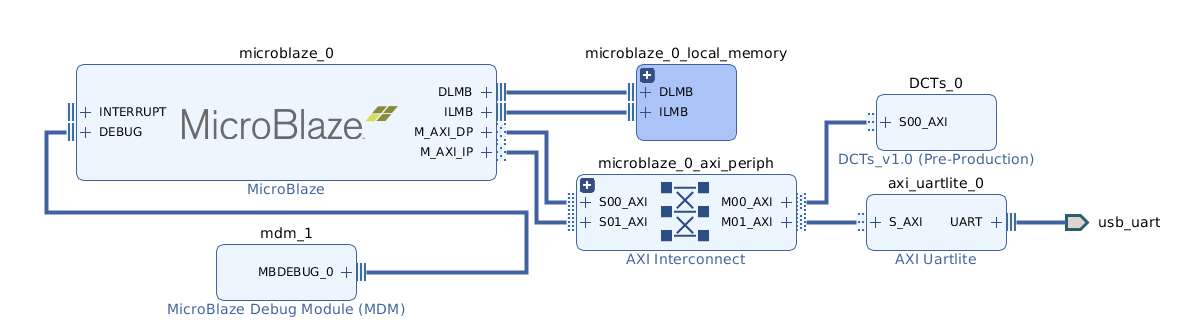
\includegraphics[width=\textwidth]{Sections/4DevelopedArchitecture/Figures/DCTCop.png}
    \caption{Block design generated by \emph{Vivado} for integration of \emph{DCT Wrapper} with \emph{Microblaze}.}
    \label{fig:blockdes}
\end{figure}

With the finalized design, some tests were developed in software, to be run on the \emph{Microblaze}. The interaction between it and the \emph{DCT Wrapper} is done with read and write routines provided by \emph{Xilinx}'s \gls{sdk}. These access the addresses attributed to the peripherals during \emph{Vivado}'s Implementation process.

The first test revolved around the verification of the calculated of coefficients. The processor injected a sequence of input vectors into the co-processor, and compared the obtained results with the software's. This short test proved successful, as the hardware implementation gave the same result as the software version for all vector sizes.

Being proven the correct calculation of the transformed coefficients, the final test was to verify the timing performances of the system. For this, a small program was written, where a vector with the same length as the desired \emph{DCT} would be loaded into the co-processor, this would be activated, and the same length transformed vector would be read back.

The most relevant result to measure was the number of clock cycles to calculate the transformed coefficients, as the read and write processes are highly dependent on the used interface. This way, in Table \ref{tab:axi4time} there are presented the separate timing results for the three different processes measured, both in number of clock cycles, as well as the time duration at the calculated maximum frequency. 

\begin{table}[!htpb]
    \centering
    \begin{tabular}{ccccccc} \toprule
        \multirow{2}{*}{\textbf{Size}}   & \multicolumn{3}{c}{\textbf{Number of Clock Cycles}$\mathbf{(T_{@101.9MHz}(ns))}$}                      \\
                                         & \textbf{Write} & \textbf{Transform} & \textbf{Read}  \\ \toprule
        \textbf{4}                       & 510 $(5005)$   & 6 $(59)$           & 462 $(4534)$   \\
        \textbf{8}                       & 902 $(8852)$   & 10 $(98)$          & 806 $(7910)$   \\
        \textbf{16}                      & 1686 $(1646)$  & 14 $(137)$         & 1494 $(14661)$ \\
        \textbf{32}                      & 3254 $(31933)$ & 18 $(177)$         & 2870 $(28165)$ \\
        \textbf{64}                      & 6390 $(62709)$ & 22 $(216)$         & 5622 $(55172)$ \\
        \bottomrule
    \end{tabular}
    \caption{Timing results for the \emph{Microblaze} integration design.}
    \label{tab:axi4time}
\end{table}

Taking the transformation times, it is possible to calculate the hypothetical throughput of the developed architecture. This is a measure of the highest frame rate this architecture could process at a given resolution. 

On a video encoder, each residue block will suffer several transformations, horizontal and vertically. Given that the presented results are referring to vector transformations, the hypothetical time for transforming a 2D block must be calculated. With the obtained results, the maximum possible frame rate of some of the most common resolutions was calculated, considering only blocks of the the corresponding size were used, giving origin to Table \ref{tab:maxfps}.

\begin{table}[!htpb]
    \centering
    \begin{tabular}{ccccc} \toprule
        \multirow{2}{*}{\textbf{Block Size}}   & \multicolumn{4}{c}{\textbf{Resolution}}                      \\
                                         & $\mathbf{1280\times 720}$    & $\mathbf{1920\times 1080}$  & $\mathbf{3840\times 2160}$  & $\mathbf{7680\times 4320}$  \\ \toprule
        $\mathbf{4\times 4}$                       & 37                      & 16                   & 4                    & 1  \\
        $\mathbf{8\times 8}$                       & 44                      & 20                   & 5                    & 1  \\
        $\mathbf{16\times 16}$                      & 63                      & 28                   & 7                    & 2  \\
        $\mathbf{32\times 32}$                      & 98                      & 44                   & 11                   & 3  \\
        $\mathbf{64\times 64}$                      & 161                     & 71                   & 18                   & 4  \\
        \bottomrule
    \end{tabular}
    \caption{Maximum frame rate for a given resolution, considering fixed square transformation blocks.}
    \label{tab:maxfps}
\end{table}

As seen, the constructed architecture, on the current hardware, isn't capable of processing high resolution video at usable frame rates. Although for HD and FHD it may be able to provide more than 30fps at some block sizes, the emerging resolutions still prove too demanding to achieve real time encoding usability. However, some works capable of delivering such performances have been published \cite{vayalilEfficientASICDesign2016,meherEfficientIntegerDCT2014,m.HighPerformanceInteger2017}.

Besides, the presented results represent a \emph{best case} scenario. On most encoders, various transformations are done on the same set of residue blocks, as to achieve the most efficient option to accomplish the target objective, be it regarding image distortion or compression. This way, efficient hardware implementations must allow this parallelization of encoding choices.

With the second version of of the \emph{DCT Wrapper}, the utilization of hardware is heavily optimized, as there are no repeated stages throughout the design. However, this makes  parallel transformations of different vector sizes impossible. Since, at least, \textbf{DCT4} will always be occupied with one of the encoding options, and as all other transform sizes need this stage to calculate its output, there isn't the possibility to calculate two different transform sizes at the same time.

However, on the decoding process, there is no need for parallelization of the Transform stage, as all the encoding options were already chosen. This way, an architecture following the same implementation would be appropriate for a decoder, where low power and size are highly desired characteristics.

On the other hand, the first version of the complete kernel had all \emph{DCT} blocks individualized, making the transformation of different sized vectors possible. As mentioned before, this makes this implementation better suited to be applied on an encoder, as it allows to test various configurations at the same time, and quickly evaluate the most adequate. However, for this to be achieved, some modifications would need to be made, as only one set of output vectors can be retrieved on the current implementation.


\clearpage
\printbibliography[heading=subbibliography]
\addcontentsline{toc}{section}{References}

%%%%%%%%%%%%%%%%%%%%%%%%%%%%%%%%%%%%%
% Developed Architecture
\cleardoublepage
\renewcommand{\thesection}{\Alph{section}}
\begin{appendices}

\section{\emph{aomenc} Configuration Options} \label{app:libaom}
\begin{lstlisting}

Usage: ./aomenc <options> -o dst_filename src_filename 

Options:
            --help                      Show usage options and exit
-c <arg>,   --cfg=<arg>                 Config file to use
-D,         --debug                     Debug mode (makes output deterministic)
-o <arg>,   --output=<arg>              Output filename
            --codec=<arg>               Codec to use
-p <arg>,   --passes=<arg>              Number of passes (1/2)
            --pass=<arg>                Pass to execute (1/2)
            --fpf=<arg>                 First pass statistics file name
            --limit=<arg>               Stop encoding after n input frames
            --skip=<arg>                Skip the first n input frames
            --good                      Use Good Quality Deadline
-q,         --quiet                     Do not print encode progress
-v,         --verbose                   Show encoder parameters
            --psnr                      Show PSNR in status line
            --webm                      Output WebM (default when WebM IO is enabled)
            --ivf                       Output IVF
            --obu                       Output OBU
-P,         --output-partitions         Makes encoder output partitions. Requires IVF output!
            --q-hist=<arg>              Show quantizer histogram (n-buckets)
            --rate-hist=<arg>           Show rate histogram (n-buckets)
            --disable-warnings          Disable warnings about potentially incorrect encode settings.
-y,         --disable-warning-prompt    Display warnings, but do not prompt user to continue.
            --test-decode=<arg>         Test encode/decode mismatch
                                        off, fatal, warn

Encoder Global Options:
            --yv12                      Input file is YV12 
            --i420                      Input file is I420 (default)
            --i422                      Input file is I422
            --i444                      Input file is I444
-u <arg>,   --usage=<arg>               Usage profile number to use
-t <arg>,   --threads=<arg>             Max number of threads to use
            --profile=<arg>             Bitstream profile number to use
-w <arg>,   --width=<arg>               Frame width
-h <arg>,   --height=<arg>              Frame height
            --forced_max_frame_width    Maximum frame width value to force
            --forced_max_frame_height   Maximum frame height value to force
            --stereo-mode=<arg>         Stereo 3D video format
                                        mono, left-right, bottom-top, top-bottom, right-left
            --timebase=<arg>            Output timestamp precision (fractional seconds)
            --fps=<arg>                 Stream frame rate (rate/scale)
            --global-error-resilient=<  Enable global error resiliency features
-b <arg>,   --bit-depth=<arg>           Bit depth for codec (8 for version <=1, 10 or 12 for version 2)
                                        8, 10, 12
            --lag-in-frames=<arg>       Max number of frames to lag
            --large-scale-tile=<arg>    Large scale tile coding (0: off (default), 1: on)
            --monochrome                Monochrome video (no chroma planes)
            --full-still-picture-hdr    Use full header for still picture

Rate Control Options:
            --drop-frame=<arg>          Temporal resampling threshold (buf %)
            --resize-mode=<arg>         Frame resize mode
            --resize-denominator=<arg>  Frame resize denominator
            --resize-kf-denominator=<a  Frame resize keyframe denominator
            --superres-mode=<arg>       Frame super-resolution mode
            --superres-denominator=<ar  Frame super-resolution denominator
            --superres-kf-denominator=  Frame super-resolution keyframe denominator
            --superres-qthresh=<arg>    Frame super-resolution qindex threshold
            --superres-kf-qthresh=<arg  Frame super-resolution keyframe qindex threshold
            --end-usage=<arg>           Rate control mode
                                        vbr, cbr, cq, q
            --target-bitrate=<arg>      Bitrate (kbps)
            --min-q=<arg>               Minimum (best) quantizer
            --max-q=<arg>               Maximum (worst) quantizer
            --undershoot-pct=<arg>      Datarate undershoot (min) target (%)
            --overshoot-pct=<arg>       Datarate overshoot (max) target (%)
            --buf-sz=<arg>              Client buffer size (ms)
            --buf-initial-sz=<arg>      Client initial buffer size (ms)
            --buf-optimal-sz=<arg>      Client optimal buffer size (ms)

Twopass Rate Control Options:
            --bias-pct=<arg>            CBR/VBR bias (0=CBR, 100=VBR)
            --minsection-pct=<arg>      GOP min bitrate (% of target)
            --maxsection-pct=<arg>      GOP max bitrate (% of target)

Keyframe Placement Options:
            --enable-fwd-kf=<arg>       Enable forward reference keyframes
            --kf-min-dist=<arg>         Minimum keyframe interval (frames)
            --kf-max-dist=<arg>         Maximum keyframe interval (frames)
            --disable-kf                Disable keyframe placement

AV1 Specific Options:
            --cpu-used=<arg>            CPU Used (0..8)
            --dev-sf=<arg>              Dev Speed (0..255)
            --auto-alt-ref=<arg>        Enable automatic alt reference frames
            --sharpness=<arg>           Loop filter sharpness (0..7)
            --static-thresh=<arg>       Motion detection threshold
            --single-tile-decoding=<ar  Single tile decoding (0: off (default), 1: on)
            --tile-columns=<arg>        Number of tile columns to use, log2
            --tile-rows=<arg>           Number of tile rows to use, log2 (set to 0 while threads > 1)
            --arnr-maxframes=<arg>      AltRef max frames (0..15)
            --arnr-strength=<arg>       AltRef filter strength (0..6)
            --tune=<arg>                Distortion metric tuned with
                                        psnr, ssim, cdef-dist, daala-dist
            --cq-level=<arg>            Constant/Constrained Quality level
            --max-intra-rate=<arg>      Max I-frame bitrate (pct)
            --max-inter-rate=<arg>      Max P-frame bitrate (pct)
            --gf-cbr-boost=<arg>        Boost for Golden Frame in CBR mode (pct)
            --lossless=<arg>            Lossless mode (0: false (default), 1: true)
            --enable-cdef=<arg>         Enable the constrained directional enhancement filter (0: false, 1: true (default))
            --enable-restoration=<arg>  Enable the loop restoration filter (0: false, 1: true (default))
            --disable-trellis-quant=<a  Disable trellis optimization of quantized coefficients (0: false (default) 1: true)
            --enable-qm=<arg>           Enable quantisation matrices (0: false (default), 1: true)
            --qm-min=<arg>              Min quant matrix flatness (0..15), default is 8
            --qm-max=<arg>              Max quant matrix flatness (0..15), default is 15
            --enable-dist-8x8=<arg>     Enable dist-8x8 (0: false (default), 1: true)
            --frame-parallel=<arg>      Enable frame parallel decodability features (0: false (default), 1: true)
            --error-resilient=<arg>     Enable error resilient features (0: false (default), 1: true)
            --aq-mode=<arg>             Adaptive quantization mode (0: off (default), 1: variance 2: complexity, 3: cyclic refresh)
            --deltaq-mode=<arg>         Delta qindex mode (0: off (default), 1: deltaq 2: deltaq + deltalf)
            --frame-boost=<arg>         Enable frame periodic boost (0: off (default), 1: on)
            --noise-sensitivity=<arg>   Noise sensitivity (frames to blur)
            --tune-content=<arg>        Tune content type
                                        default, screen
            --cdf-update-mode=<arg>     CDF update mode for entropy coding (0: no CDF update; 1: update CDF on all frames(default); 2: selectively update CDF on some frames
            --color-primaries=<arg>     Color primaries (CICP) of input content:
                                        bt709, unspecified, bt601, bt470m, bt470bg, smpte240, film, bt2020, xyz, smpte431, smpte432, ebu3213
            --transfer-characteristics  Transfer characteristics (CICP) of input content:
                                        unspecified, bt709, bt470m, bt470bg, bt601, smpte240, lin, log100, log100sq10, iec61966, bt1361, srgb, bt2020-10bit, bt2020-12bit, smpte2084, hlg, smpte428
            --matrix-coefficients=<arg  Matrix coefficients (CICP) of input content:
                                        identity, bt709, unspecified, fcc73, bt470bg, bt601, smpte240, ycgco, bt2020ncl, bt2020cl, smpte2085, chromncl, chromcl, ictcp
            --chroma-sample-position=<  The chroma sample position when chroma 4:2:0 is signaled:
                                        unknown, vertical, colocated
            --min-gf-interval=<arg>     min gf/arf frame interval (default 0, indicating in-built behavior)
            --max-gf-interval=<arg>     max gf/arf frame interval (default 0, indicating in-built behavior)
            --sb-size=<arg>             Superblock size to use
                                        dynamic, 64, 128
            --num-tile-groups=<arg>     Maximum number of tile groups, default is 1
            --mtu-size=<arg>            MTU size for a tile group, default is 0 (no MTU targeting), overrides maximum number of tile groups
            --timing-info=<arg>         Signal timing info in the bitstream (model unly works for no hidden frames, no super-res yet):
                                        unspecified, constant, model
            --film-grain-test=<arg>     Film grain test vectors (0: none (default), 1: test-1  2: test-2, ... 16: test-16)
            --film-grain-table=<arg>    Path to file containing film grain parameters
            --enable-ref-frame-mvs=<ar  Enable temporal mv prediction (default is 1)
-b <arg>, --bit-depth=<arg>           Bit depth for codec (8 for version <=1, 10 or 12 for version 2)
                                        8, 10, 12
            --input-bit-depth=<arg>     Bit depth of input
            --sframe-dist=<arg>         S-Frame interval (frames)
            --sframe-mode=<arg>         S-Frame insertion mode (1..2)
            --annexb=<arg>              Save as Annex-B

Stream timebase (--timebase):
The desired precision of timestamps in the output, expressed
in fractional seconds. Default is 1/1000.

Included encoders:

av1    - AOMedia Project AV1 Encoder v0.1.0 (default)

    Use --codec to switch to a non-default encoder.
\end{lstlisting}

%%%%%%%%%%%%%%%%%%%%%%%%%%%%%%%%%%%%%%%%%%%%%%%%%%%%%%%%%%%%%%%%%%%%%%%%%%%
\section{DCT8\_1 VHDL Description} \label{app:dct81}
\begin{lstlisting}[style=vhdl]
-- DCT8 Implementation for inetgration with aggregated architecture

library IEEE;
use IEEE.STD_LOGIC_1164.ALL;
use IEEE.NUMERIC_STD.ALL;
use IEEE.STD_LOGIC_UNSIGNED.ALL;

entity DCT8_1_I is
port(   -- Data Inputs
    dataIn0     : in    integer;
    dataIn1     : in    integer;
    dataIn2     : in    integer;
    dataIn3     : in    integer;
    dataIn4     : in    integer;
    dataIn5     : in    integer;
    dataIn6     : in    integer;
    dataIn7     : in    integer;
    -- Control Inputs
    res         : in    std_logic;
    en          : in    std_logic;
    clk         : in    std_logic;
    -- Data Outputs
    dataOut0    : out    integer;
    dataOut1    : out    integer;
    dataOut2    : out    integer;
    dataOut3    : out    integer;
    dataOut4    : out    integer;
    dataOut5    : out    integer;
    dataOut6    : out    integer;
    dataOut7    : out    integer;
    -- Control Outputs
    validOut    : out   std_logic
);
end DCT8_1_I;

architecture Behavioral of DCT8_1_I is
begin

stage1:     process(clk, res, en)
        begin
            if(rising_edge(clk)) then
                if(res = '1') then
                    dataOut0 <= 0;
                    dataOut1 <= 0;
                    dataOut2 <= 0;
                    dataOut3 <= 0;
                    dataOut4 <= 0;
                    dataOut5 <= 0;
                    dataOut6 <= 0;
                    dataOut7 <= 0;
                    validOut <= '0';
                elsif(en = '1') then
                    dataOut0 <= dataIn0 + dataIn7;
                    dataOut1 <= dataIn1 + dataIn6;
                    dataOut2 <= dataIn2 + dataIn5;
                    dataOut3 <= dataIn3 + dataIn4;
                    dataOut4 <= dataIn3 - dataIn4;
                    dataOut5 <= dataIn2 - dataIn5;
                    dataOut6 <= dataIn1 - dataIn6;
                    dataOut7 <= dataIn0 - dataIn7;
                    validOut <= '1';
                end if;
            end if;
        end process;
end Behavioral;
\end{lstlisting}

%%%%%%%%%%%%%%%%%%%%%%%%%%%%%%%%%%%%%%%%%%%%%%%%%%%%%%%%%%%%%%%%%%%%%%%%%%%
\section{DCT8\_2 VHDL Description} \label{app:dct82}
\begin{lstlisting}[style=vhdl]
-- DCT8 Stage 2 Implementation for integration with aggregated architecture

library IEEE;
use IEEE.STD_LOGIC_1164.ALL;
use IEEE.NUMERIC_STD.ALL;
use IEEE.STD_LOGIC_UNSIGNED.ALL;

entity DCT8_2_I is
port(   -- Data Inputs
    dataIn4     : in    integer;
    dataIn5     : in    integer;
    dataIn6     : in    integer;
    dataIn7     : in    integer;
    -- Control Inputs
    res         : in    std_logic;
    en          : in    std_logic;
    clk         : in    std_logic;
    -- Data Outputs
    dataOut4    : out    integer;
    dataOut5    : out    integer;
    dataOut6    : out    integer;
    dataOut7    : out    integer;
    -- Control Outputs
    validOut    : out   std_logic
);
end DCT8_2_I;

architecture Behavioral of DCT8_2_I is
signal s_stg2M5, s_stg2M6       :   integer := 0;
signal s_stg2A5, s_stg2A6       :   integer := 0;
signal s_stg2D5, s_stg2D6       :   integer := 0;
signal s_stg34, s_stg35, s_stg36, s_stg37       :   integer := 0;
signal s_stg4M41, s_stg4M42, s_stg4M51, s_stg4M52, s_stg4M61, s_stg4M62, s_stg4M71, s_stg4M72       :   integer := 0;
signal s_stg4A4, s_stg4A5, s_stg4A6, s_stg4A7       :   integer := 0;
signal s_stage2MEn, s_stage2AEn, s_stage2DEn, s_stage3En, s_stage4MEn, s_stage4AEn, s_valOut       :   std_logic := '0';
begin

stage2M:    process(clk, res, en)
        begin
            if(rising_edge(clk)) then
                if(res = '1') then
                    s_stg2M5 <= 0;
                    s_stg2M6 <= 0;
                    s_stage2AEn <= '0';
                elsif(en = '1') then
                    s_stg2M5 <= dataIn5*185;
                    s_stg2M6 <= dataIn6*185;
                    s_stage2AEn <= '1';
                end if;
            end if;
        end process;

stage2A:    process(clk, res, s_stage2AEn)
        begin
            if(rising_edge(clk)) then
                if(res = '1') then
                    s_stg2A5 <= 0;
                    s_stg2A6 <= 0;
                    s_stage2DEn <= '0';
                elsif(s_stage2AEn = '1') then
                    s_stg2A5 <= s_stg2M6 - s_stg2M5;
                    s_stg2A6 <= s_stg2M6 + s_stg2M5;
                    s_stage2DEn <= '1';
                end if;
            end if;
        end process;

stage2D:    process(clk, res, s_stage2DEn)
        begin
            if(rising_edge(clk)) then
                if(res = '1') then
                    s_stg2D5 <= 0;
                    s_stg2D6 <= 0;
                    s_stage3En <= '0';
                elsif(s_stage2DEn = '1') then
                    s_stg2D5 <= to_integer(shift_right(to_signed(s_stg2A5,32),8));
                    s_stg2D6 <= to_integer(shift_right(to_signed(s_stg2A6,32),8));
                    s_stage3En <= '1';
                end if;
            end if;
        end process;                

stage3:     process(clk, res, s_stage3En)
        begin
            if(rising_edge(clk)) then
                if(res = '1') then
                    s_stg34 <= 0;
                    s_stg35 <= 0;
                    s_stg36 <= 0;
                    s_stg37 <= 0;
                    s_stage4MEn <= '0';
                elsif(s_stage3En = '1') then
                    s_stg34 <= dataIn4 + s_stg2D5;
                    s_stg35 <= dataIn4 - s_stg2D5;
                    s_stg36 <= dataIn7 - s_stg2D6;
                    s_stg37 <= dataIn7 + s_stg2D6;
                    s_stage4MEn <= '1';
                end if;
            end if;
        end process;

stage4M:    process(clk, res, s_stage4MEn)
        begin
            if(rising_edge(clk)) then
                if(res = '1') then
                    s_stg4M41 <= 0;
                    s_stg4M42 <= 0;
                    s_stg4M51 <= 0;
                    s_stg4M52 <= 0;
                    s_stg4M61 <= 0;
                    s_stg4M62 <= 0;
                    s_stg4M71 <= 0;
                    s_stg4M72 <= 0;
                    s_stage4AEn <= '0';
                elsif(s_stage4MEn = '1') then
                    s_stg4M41 <= s_stg34*56;
                    s_stg4M42 <= s_stg34*252;
                    s_stg4M51 <= s_stg35*147;
                    s_stg4M52 <= s_stg35*216;
                    s_stg4M61 <= s_stg36*147;
                    s_stg4M62 <= s_stg36*216;
                    s_stg4M71 <= s_stg37*56;
                    s_stg4M72 <= s_stg37*252;
                    s_stage4AEn <= '1';
                end if;
            end if;
        end process;

stage4A:    process(clk, res, s_stage4AEn)
        begin
            if(rising_edge(clk)) then
                if(res = '1') then
                    s_stg4A4 <= 0;
                    s_stg4A5 <= 0;
                    s_stg4A6 <= 0;
                    s_stg4A7 <= 0;
                    s_valOut <= '0';
                elsif(s_stage4AEn = '1') then
                    s_stg4A4 <= s_stg4M41 + s_stg4M72;
                    s_stg4A5 <= s_stg4M52 + s_stg4M61;
                    s_stg4A6 <= s_stg4M62 - s_stg4M51;
                    s_stg4A7 <= s_stg4M71 - s_stg4M42;
                    s_valOut <= '1';
                end if;
            end if;
        end process;
        
outReg:     process(clk, res, s_valOut)
        begin
            if(rising_edge(clk)) then
                if(res = '1') then
                    dataOut5 <= 0;
                    dataOut6 <= 0;
                    dataOut7 <= 0;
                    validOut <= '0';
                elsif(s_valOut = '1') then
                    dataOut4 <= to_integer(shift_right(to_signed(s_stg4A4,32),8));
                    dataOut5 <= to_integer(shift_right(to_signed(s_stg4A5,32),8));
                    dataOut6 <= to_integer(shift_right(to_signed(s_stg4A6,32),8));
                    dataOut7 <= to_integer(shift_right(to_signed(s_stg4A7,32),8));
                    validOut <= '1';
                end if;
            end if;
        end process;
end Behavioral;
\end{lstlisting}
\end{appendices}


%%%%%%%%%%%%%%%%%%%%%%%%%%%%%%%%%%%%%
% Bibliografia
%\cleardoublepage
%  \nocite{*}
%  \printbibliography
%\cleardoublepage

\end{document}
